\documentclass[10pt, a4paper, twocolumn]{article} 
\usepackage[T1]{fontenc}
\usepackage[utf8]{inputenc}
\usepackage[english]{babel}

\usepackage[left=1.55cm, right=1.55cm, top=2.25cm, bottom=2.25cm, headheight=11pt, letterpaper]{geometry}
\setlength{\columnsep}{0.50cm} % Distance between the two columns of text

\usepackage{graphicx}
\graphicspath{{Figures/}{./}}
\usepackage[inline]{enumitem}
\usepackage{csquotes}
\usepackage{microtype}
\usepackage{xcolor}
\usepackage{siunitx}
\sisetup{output-exponent-marker=\ensuremath{\mathrm{e}}}
\usepackage{lastpage}
\usepackage{tabularx,booktabs}
\usepackage{amsmath, amsfonts, amssymb}
\usepackage{pdfpages}
\usepackage{indentfirst}
\usepackage{lipsum}
\usepackage{multirow}
\usepackage{adjustbox}
\usepackage{comment}
\usepackage{caption}
\usepackage{subcaption}
\usepackage{float}

\usepackage[labelfont={bf,sf,small}, labelsep=period, format = plain, justification=justified]{caption}
\setlength{\abovecaptionskip}{3pt}
\setlength{\belowcaptionskip}{0pt}

\usepackage{fancyhdr} % Needed to define custom headers/footers
\pagestyle{fancy} % Enables the custom headers/footers
\renewcommand{\headrulewidth}{0pt} % No header rule
\renewcommand{\footrulewidth}{0pt}
\lhead{}
\chead{}
\rhead{\small\sffamily\bfseries\ Human Activity Recognition Using Smartphones --- \thepage/\pageref{LastPage}}
\lfoot{}
\cfoot{}
\rfoot{}

\usepackage[style=authoryear-icomp,maxbibnames=99,maxcitenames=2,uniquelist=false,isbn=false,backend=biber]{biblatex}
\addbibresource{biblio.bib}

\definecolor{color1}{RGB}{0,0,0} % Color of the article title and sections
\definecolor{color2}{RGB}{0,20,20} % Color of the boxes behind the abstract and headings

\usepackage{hyperref}
\hypersetup{%
	linktoc=page,%
	colorlinks = true,%
	linkcolor=[cmyk]{1, 0.50, 0, 0},%
	anchorcolor=[cmyk]{1, 0.50, 0, 0},%
	citecolor=[rgb]{0,0.5,0},%	
	filecolor=[cmyk]{1, 0.50, 0, 0},%
	menucolor=[cmyk]{1, 0.50, 0, 0},%
	runcolor=[cmyk]{1, 0.50, 0, 0},%
	urlcolor=[rgb]{0.6,0,0},%
	pdfinfo={%
		Author={Simone Di Luna, Lia Trapanese, Giulio Cordova},%
		Title={Human Activity Recognition Using Smartphones},%
		Subject={},%
		Keywords={},%
		CreationDate={D:20220217170000},%
		ModDate={},%		
	}
}

% stampa doi invece di url se presenti entrambi. Stampa url se non c'è doi
\renewbibmacro*{doi+eprint+url}{%
	\printfield{doi}%
	\newunit\newblock%
	\iftoggle{bbx:eprint}{%
		\usebibmacro{eprint}%
	}{}%
	\newunit\newblock%
	\iffieldundef{doi}{%
		\usebibmacro{url+urldate}}%
	{}%
}

% \citeyear cliccabile
\DeclareCiteCommand{\citeyear}
{\usebibmacro{prenote}}
{\bibhyperref{\printfield{year}}\bibhyperref{\printfield{extrayear}}}
{\multicitedelim}
{\usebibmacro{postnote}}

\DeclareCiteCommand{\citeyearpar}[\mkbibparens]
{\usebibmacro{prenote}}
{\bibhyperref{\printfield{year}}\bibhyperref{\printfield{extrayear}}}
{\multicitedelim}
{\usebibmacro{postnote}}

\pdfsuppresswarningpagegroup=1 %rimuovere il worning quando si caricano più pdf

\usepackage{newtxtext, newtxmath}

\begin{document}
	
\setlength{\topmargin}{-1cm}
\setlength{\textheight}{240mm}
\setlength{\textwidth}{142mm}
\setlength{\evensidemargin}{0.3in}
\setlength{\oddsidemargin}{0.3in}
%\setlength\parindent{4pt}
\newcommand{\Rom}[1]{\uppercase\expandafter{\romannumeral#1}}
	
\begin{titlepage}
	\begin{center}
		
\includegraphics[scale=.5]{FrontespizioDM2/marchio_unipi_pant541.eps} \\\vspace{15pt}
		\LARGE \textsc{Department of Computer Science} \\
		\Large Data Science and Business Informatics
		\vskip 0.7in
		\Large Data Mining \Rom{2} Project \\
		\vskip 1in
		{\fontsize{30}{36}\selectfont Human Activity Recognition Using Smartphones}
		
		\vskip 1in
		
		    
		    {\Large Lia Trapanese 628153}\\
		\par{\Large Simone Di Luna 544322}\\
		\par{\Large Giulio Cordova 588294}  
		
	    \vfill
	
	    \centering
	    \large Academic year 2021/2022
	\end{center}		
\end{titlepage}
\restoregeometry

\tableofcontents
\thispagestyle{empty}

\section*{Introduction}%\label{sec:imblearning}

The \citetitle{har:2012} \parencite{har:2012} is a data set related to an experiment conducted on 30 volunteers aged 19 to 48 years. The experiment consisted in making people perform six activities ---WALKING, WALKING UPSTAIRS, WALKING DOWNSTAIRS, SITTING, STANDING, LAYING---wearing a smartphone (Samsung Galaxy S \Rom{2}) on the waist.

The two measured physical quantities were the 3-axial velocity and the 3-axial acceleration. These were captured at a rate of 50 Hz using the embedded accelerometer and gyroscope of the cellphone. The experiment was video-recorded to manually label the data. Subsequently, data were randomly partitioned into two sets: 70\% of the volunteers were allocated to the train set and 30\% to the test data. 

The feature engineered dataset on which we focused on the first part of this project was built in the following way. To avoid noise, a low-pass filter was applied to signals which were then sampled in fixed-width sliding windows of 2.56 sec and 50\% overlap (128 readings per window). Another low-pass filter at a lower cutoff frequency was used to separate the gravitational and body motion component. From each window, a vector of features was obtained by calculating variables from the time domain. Instead, for what concern the variables in the frequency domain, the authors applied a Fast Fourier Transform to same of the signals.

Overall, the number of engineered features is 561. The train set contains 7352 objects, while the test set 2947.

\section{Exploratory Data Analysis}

In this section, we explore and prepare the dataset for further analysis. First, the outliers were detected with various techniques and treated according to the analysis. Then, due to the huge number of features, a dimensionality reduction was performed. Lastly, to test imbalanced learning algorithms, we manually unbalanced the dataset. Finally, we addressed to multi-class classification tasks.

\subsection{Data Understanding}\label{subsec:data_understanding}

In this first part of the project, we focus on the dataset with 561 engineered features. 

\begin{figure}
    \centering
    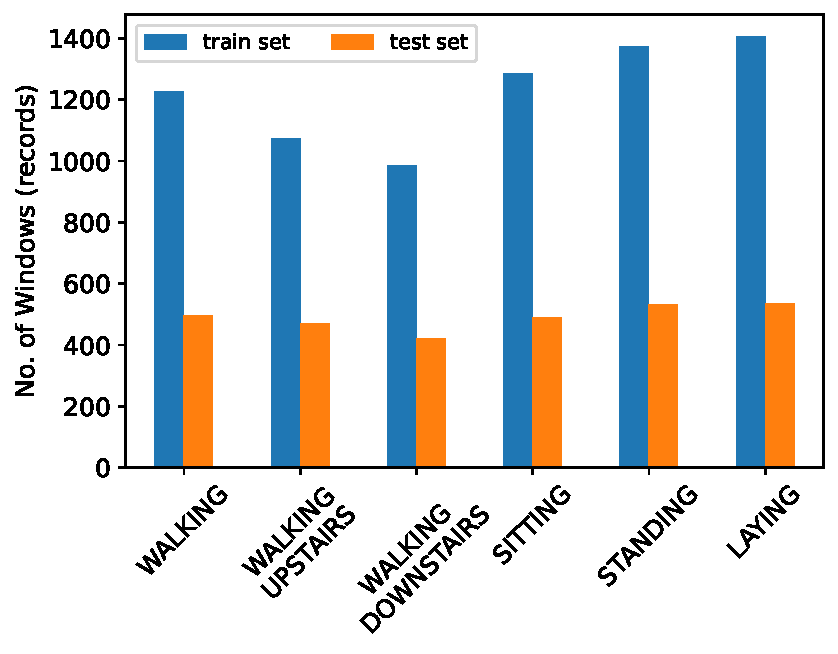
\includegraphics[width=0.7\linewidth]{immagini simone/cardinality_datasets.pdf}
    \caption{Cardinality with respect to each class on both train and test set.}
    \label{fig:cardinality}
\end{figure}

The attributes in the dataset were already normalized in range $[-1,1]$. For what concern data completeness, the dataset does not present null nor missing values. Moreover, data are both syntactically and semantically correct since all features are numerical and within their defined domain. However, as reported in the official documentation, data are collected manually, thus we cannot exclude the presence of measurement and transcription errors. For these reasons, data precision could be limited. 

Checking the correlations among the variables in the dataset, we noted that some of them share a perfect correlation. This does not surprise us, since the defined statistical quantities are not independent from each other. Going deeper into the issue, we discovered that there were many duplicated columns. In the end, we identify 19 groups of variables sharing the same identical values. Hence, we proceeded to clean up the dataset by removing 21 duplicate columns, leaving only one of them for each group. This allowed us to reduce the dimensionality of the dataset from 561 to 540 attributes.

By looking at Figure~\ref{fig:cardinality}, we can also notice that classes are quite balanced, therefore there is no need to use any imbalanced techniques.

\begin{figure}


  \begin{subfigure}[t]{0.49\columnwidth}
    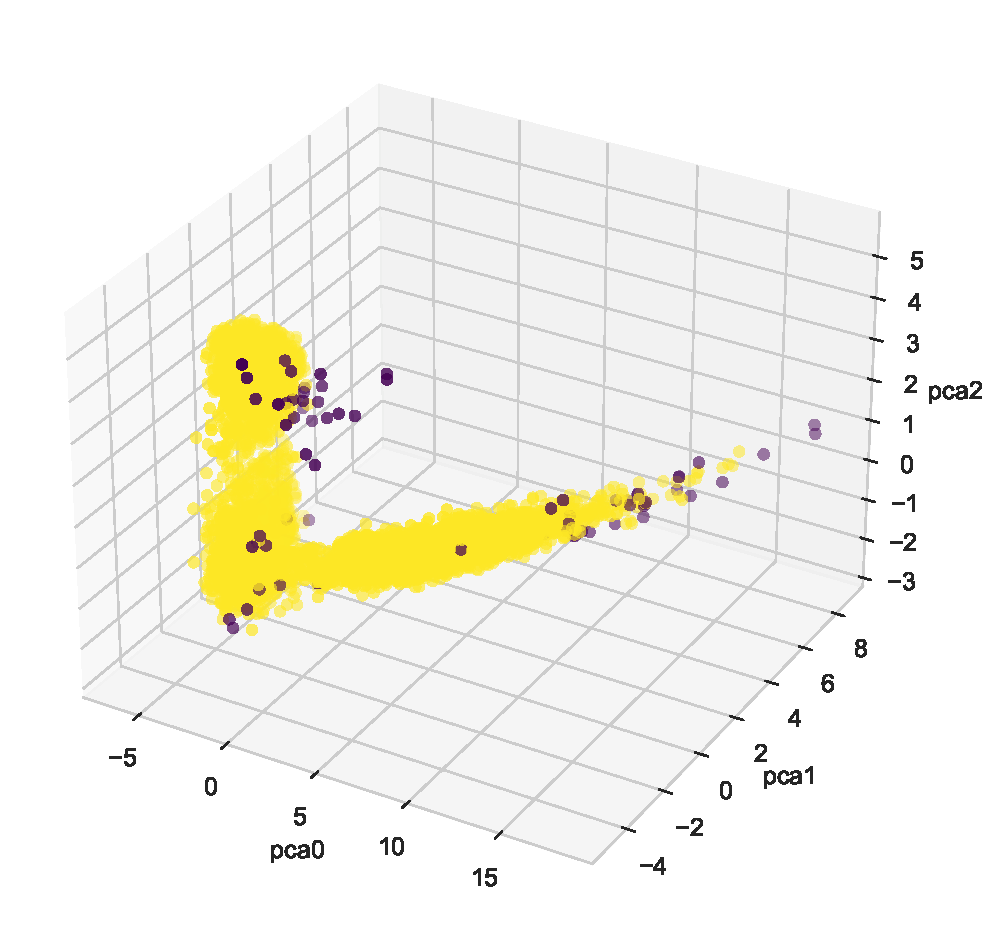
\includegraphics[width=\linewidth]{immagini Lia/DBSCAN_anomaly_detection1.pdf}
    \caption{DBSCAN}
    \label{fig:dbscan}
  \end{subfigure}
  \hfill %%
  \addtocounter{subfigure}{2}
  \begin{subfigure}[t]{0.49\columnwidth}
    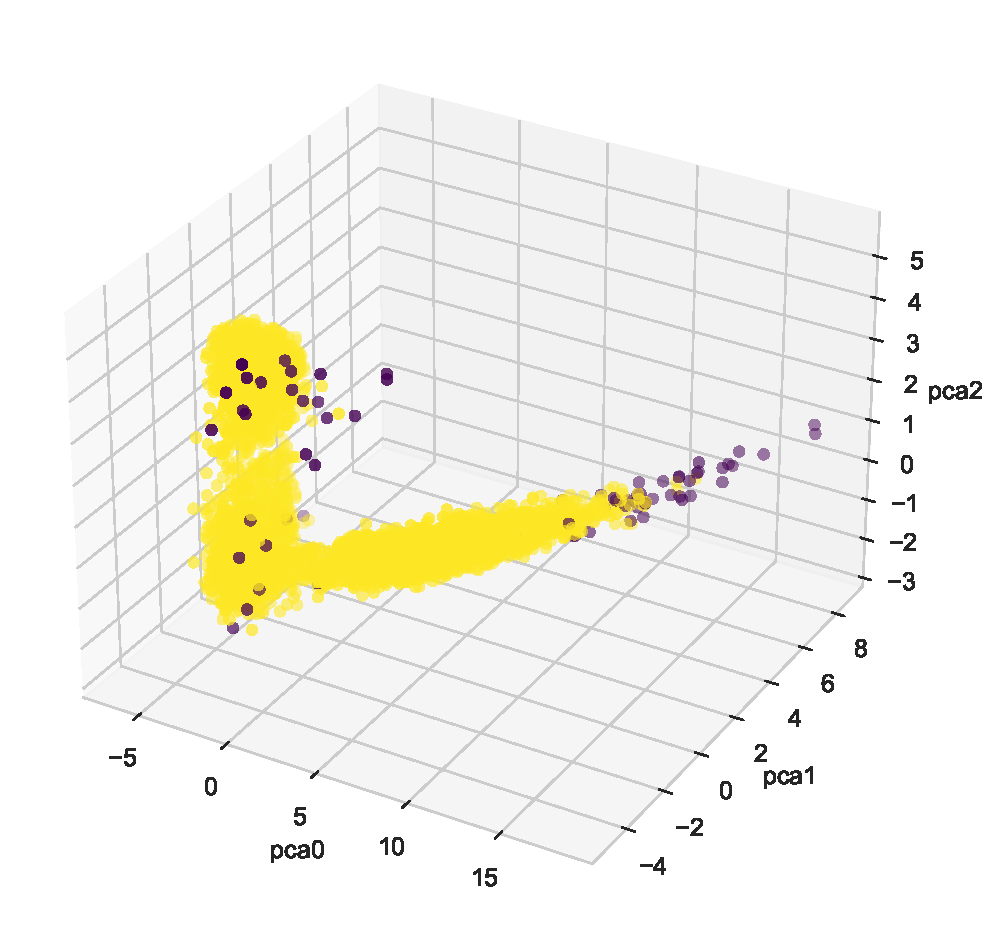
\includegraphics[width=\linewidth]{immagini Lia/ABOD_anomaly_detection.pdf} 
    \caption{ABOD}
    \label{fig:abod}
  \end{subfigure}

\addtocounter{subfigure}{-3}
  \begin{subfigure}[t]{0.49\columnwidth}
    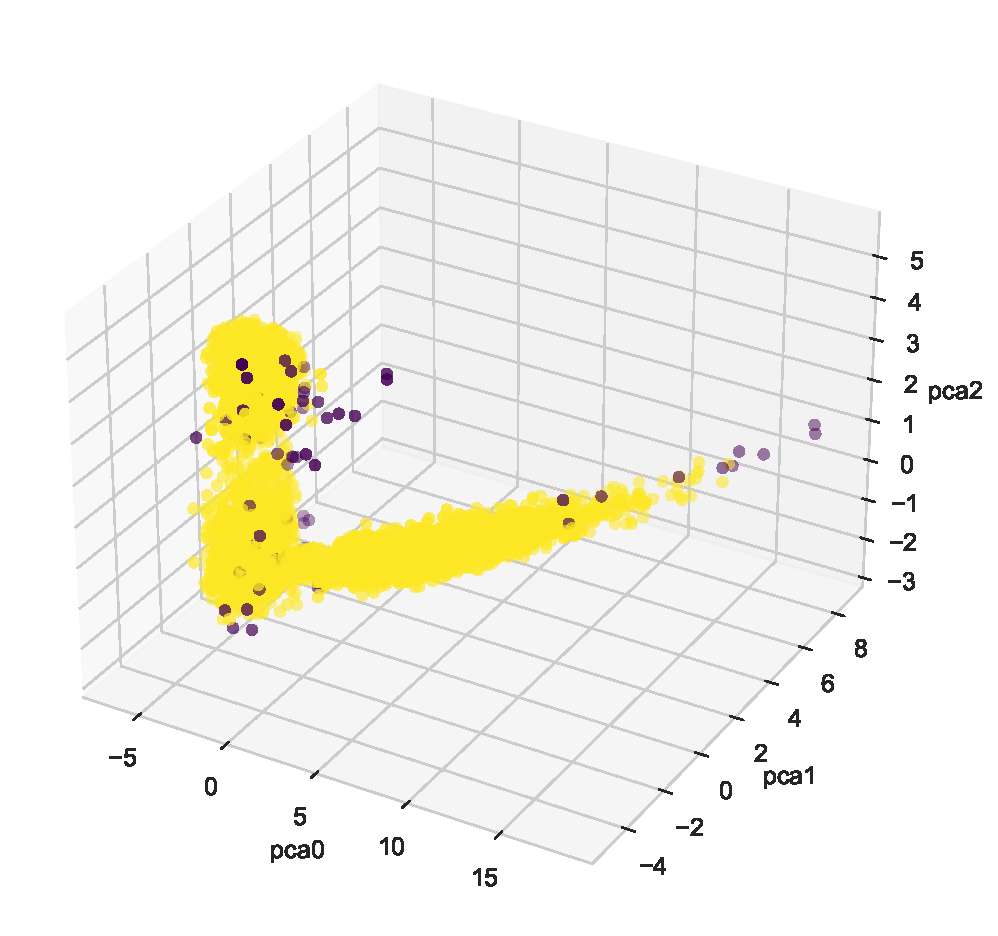
\includegraphics[width=\linewidth]{immagini Lia/LOF_anomaly_detection.pdf}
    \caption{LOF}
    \label{fig:lof}
  \end{subfigure}
  \hfill %%
  \addtocounter{subfigure}{2}
    \begin{subfigure}[t]{0.49\columnwidth}
    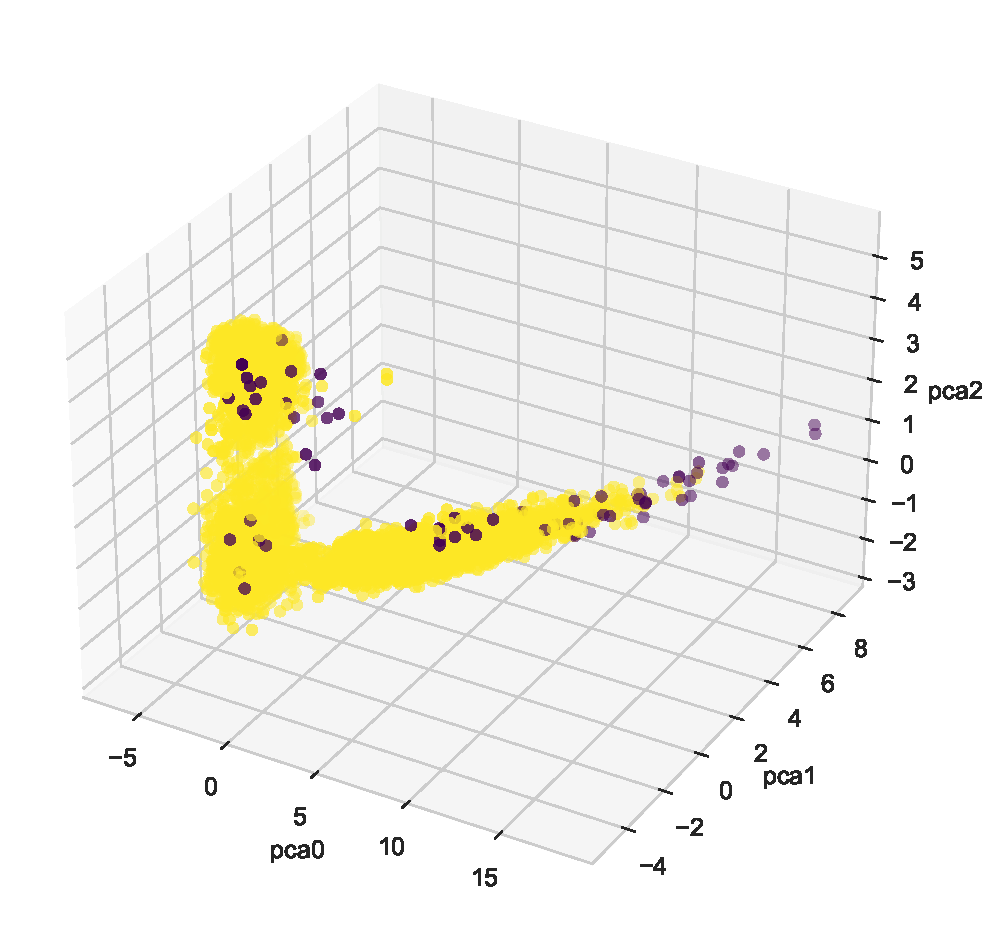
\includegraphics[width=\linewidth]{immagini Lia/Iso_anomaly_detection.pdf}
    \caption{Isolation Forest}
    \label{fig:iso}
  \end{subfigure}

\addtocounter{subfigure}{-3}  
  \begin{subfigure}[t]{0.49\columnwidth}
    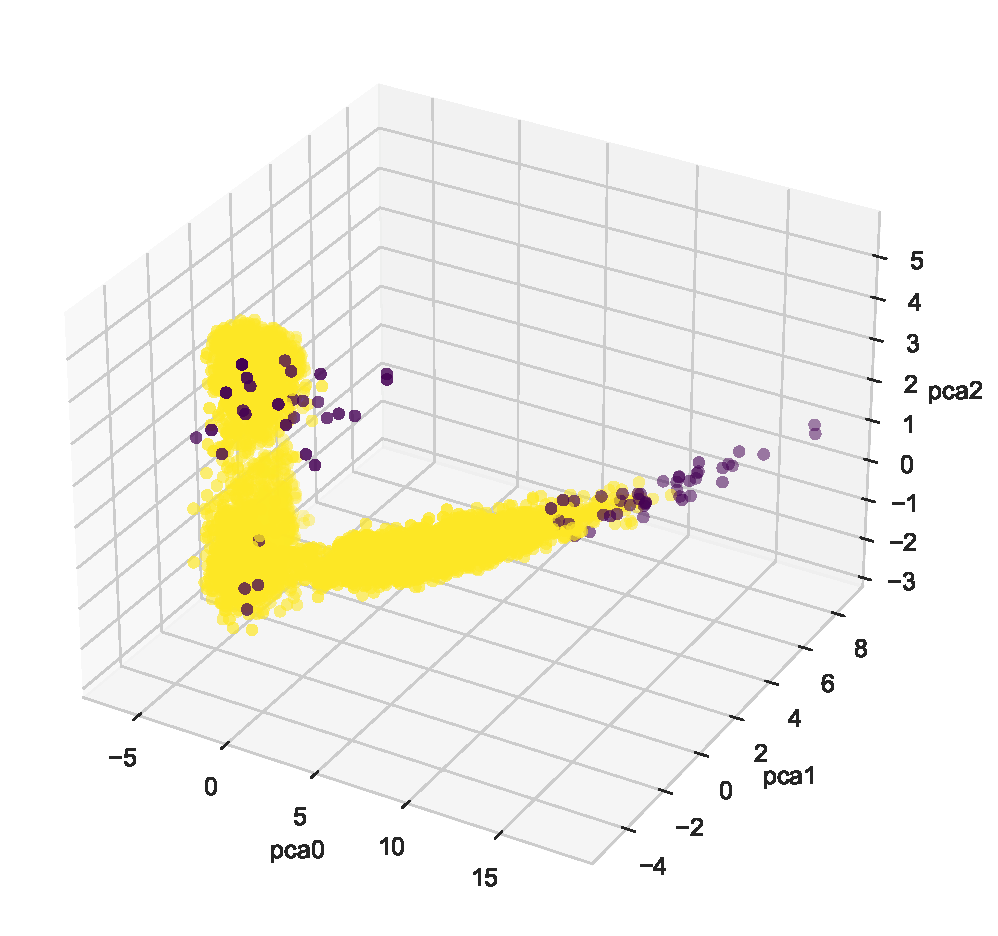
\includegraphics[width=\linewidth]{immagini Lia/KNN_anomaly_detection.pdf}
    \caption{KNN}
    \label{fig:KNN}
  \end{subfigure}
 \hfill %%
\addtocounter{subfigure}{2}
  \begin{subfigure}[t]{0.49\columnwidth}
    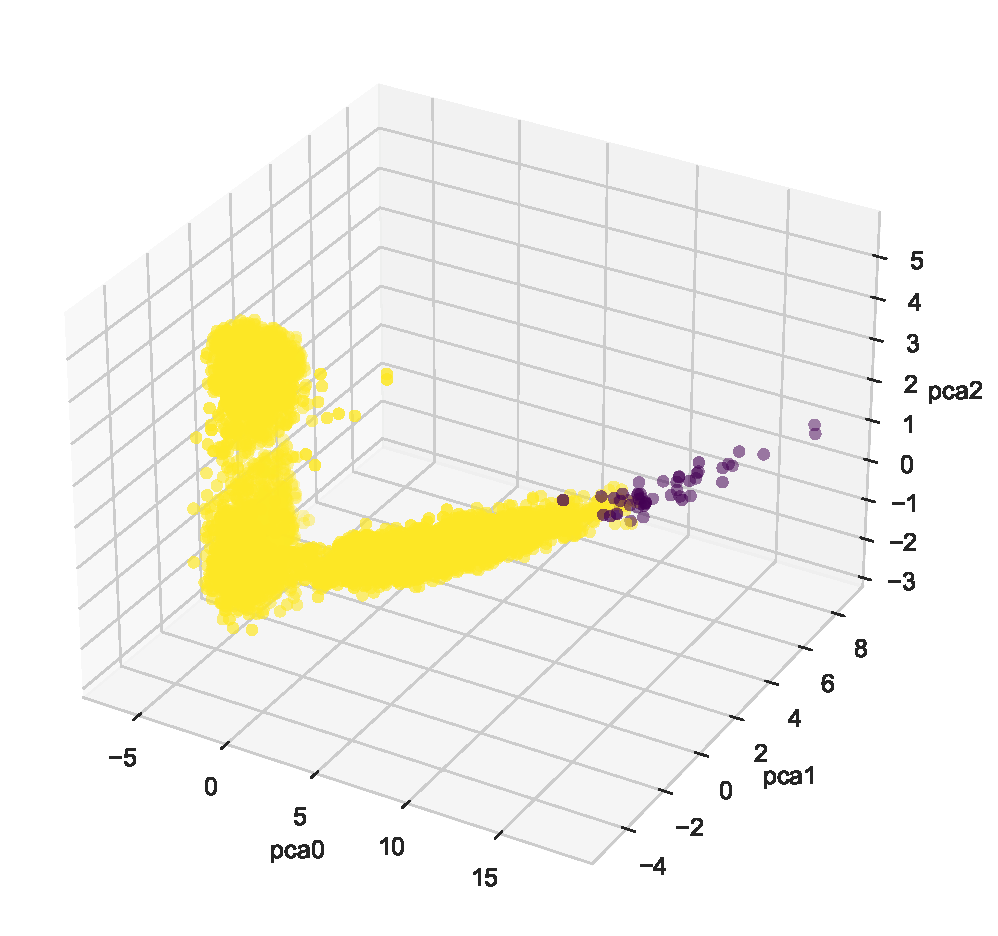
\includegraphics[width=\linewidth]{immagini Lia/EX_Iso_anomaly_detection.pdf}
    \caption{Extended Isolation Forest}
    \label{fig:exiso}
  \end{subfigure}
  
  \caption{Anomaly Detection}
  \label{fig:anomaly}
\end{figure}

\subsection{Outlier Detection}

In this section, we used many different outlier detection algorithms. Since we did not want to rely on just one method, we constructed an ensemble that provided us with a more accurate outlier labeling, i.e. using majority voting. 

Considering that some of the algorithms adopts metrics which are meaningless in high dimensions, we tested their performance both on PCA projections and on the fully-dimensional dataset. For the first one, features were selected by choosing the number of components that can explain at least 90\% of the variance in the data so that no information is lost. We performed the PCA with the 33 chosen components and we inspected the data distribution with the help of 2d and 3d scatter plots. The obtained dataset was then employed in the following anomaly detection algorithms: DBSCAN, LOF, KNN. To detect additional outliers in the data, the full-dimensional dataset consisting of 540 features was used with the ABOD, Isolation Forest, and Extended Isolation Forest algorithms.

Moreover, we also applied both univariate---Grubbs' test, the Likelihood approach--- and multivariate statistical approaches, as well as a depth-based technique.

\subsubsection*{Result of the Analysis}

Before removing the outliers, our dataset consisted of 7352 records. After analyzing the distribution of our data, we identified the top 1\% outliers using a contamination parameter to instruct the algorithms in identifying only the specified portion of anomalies.

The anomaly detection using DBSCAN and KNN was performed after the hyper-parameter tuning needed to find the right configuration. For DBSCAN the right configuration setting was identified with $\varepsilon = 3.4$ and $min sample = 3$. We noticed that as we reduced the radius and increased the $min samples$, most of the data were incorrectly labeled as outliers. KNN performed best when the number of neighbors was set to 30. For the LOF algorithm, this parameter returned better results when set to 50. The ABOD algorithm was performed on the full dataset, since it is a multidimensional approach, hence not sensible to high dimensionality. For the latter, we have set the number of neighbors equal to 50. 

We noticed that some of the outliers obtained by these four methods perfectly matched, which means that the choice of parameters is optimal. For example, both ABOD and KNN show almost the same outliers particularly in the right part of the scatter plot of the distribution in Figure \ref{fig:anomaly}.

We also tested the Isolation Forest (IF)---comparing the implementation of both sklearn and eif libraries---and the Extended Isolation Forest (EIF). The isolation forest was built using 1000 classifiers with a sample size of 256, while the extended isolation forest was built with 600 classifiers. We tested the isolation forest on both datasets: on the one built using the PCA and on the original dataset. We discovered that both returned the same number of outliers, however, some of the points identified as outliers were different.  

The extended isolation forest, compared to other methods shows a decrease in the number of outliers, hence it identifies more inliers.

On the other hand, the statistical approaches can only be applied to those attributes having a normal distribution. Therefore, as a preliminary step, we went in search of normal features. 

To check for normality, we applied three different statistical tests and, after visually verifying the correctness of the outputs through histograms and Q-Q plots, we chose only those variables unanimously labeled as normal.

Specifically, we used the following functions provided by the scipy library: D’Agostino and Pearson’s test, Shapiro-Wilk test, and Anderson test. Namely, these functions test the null hypothesis that a variable comes from a normal distribution. Hence, if the p-value is smaller than the significance level, the attribute under investigation can be considered non-normal. Eventually, we ended up with 15 normal attributes. 

Grubbs' is a univariate test that uses an iterative procedure. At each iteration, it computes the z-scores based on the current set of values. The value with the largest z-score is discarded if its z-score is larger than the critical value of the test based on the significance level chosen. This process is repeated until no objects are eliminated. We implemented the algorithm from the scratch and using a significance value of 5\% we found 2 outliers.

On the other hand, the likelihood approach assumes that the data come from two different distributions and thus applies the maximum likelihood. Specifically, it maximizes the probability that the data come from two different distributions: a normal distribution and a uniform distribution (the outliers).

Like Grubbs, this is a univariate approach. Also here, we implemented the algorithm from scratch. We assumed a fraction of outliers in the train set equal to 1\%. Moreover, we fixed a threshold value equal to 3. With these hyperparameters, the algorithm found 13 outliers.

The two statistical approaches just described, are univariate and thus they have to be repeated on each normal attribute. However, we can also use approaches that take into account all the normal attribute at the same time.

\begin{comment}
\begin{figure}
    \centering
    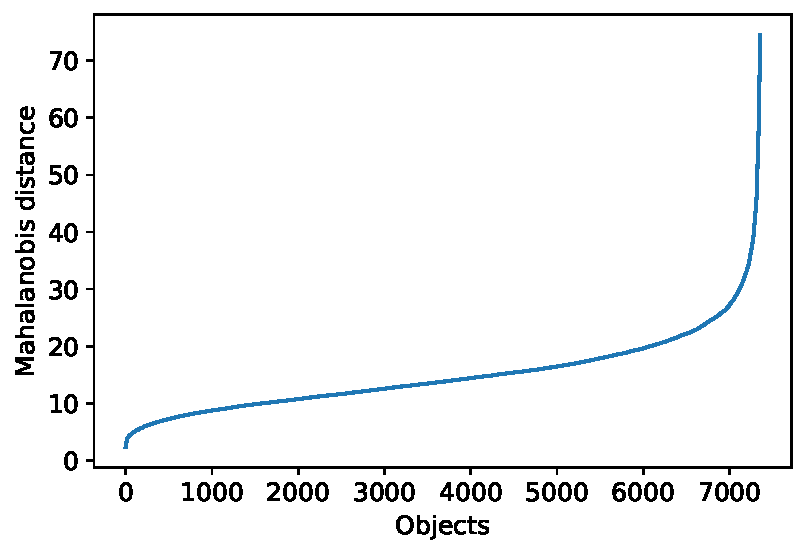
\includegraphics[width=0.60\linewidth]{immagini simone/output_65_0.pdf}
    \caption{Distances with respect to the center of the multivariate Gaussian distribution.}
    \label{fig:mahal_dists}
\end{figure}
\end{comment}

\begin{figure}
    \centering
    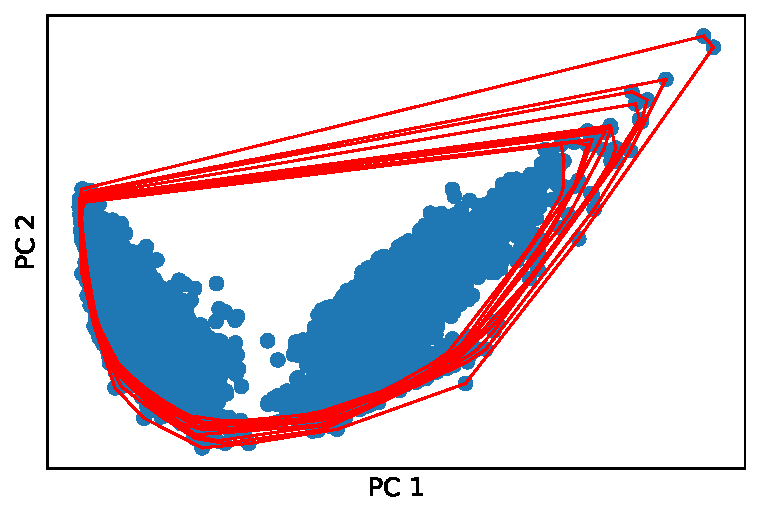
\includegraphics[width=0.6\linewidth]{immagini simone/output_75_0.pdf}
    \caption{Convex hull layers from depth 1 to 10.}
    \label{fig:convex_hull}
\end{figure}

Specifically, we can use the Mahalanobis distance to measure the distance of each point from the center of the multivariate Gaussian distribution. Then, according to a specified threshold, we can consider as outliers the objects having a larger distance. The Mahalanobis distance take into account the covariance between normal attributes and can be computed as $M(x, \bar{x})~=~(x- \bar{x})\boldsymbol{C}^{-1}(x - \bar{x})^T$, where $x$ is a generic point, $\bar{x}$ is the mean of the data, while $\boldsymbol{C}^{-1}$ is the inverse of the covariance matrix of the data. 

To decide which objects to remove, we sorted all points according to their Mahalanobis distance and then we plotted the resulting graph. In the end, we decided to consider as outliers the 4 points having the largest Mahalanobis distance.

Eventually, we used depth-based approaches. This approach does not make any assumption on the statistical distribution of the variables and thus can be used on the whole attributes space. Specifically, this approach plot the data in a 2d or 3d space and then assumes that data at the border of the region are outliers.

To apply this technique, we first transformed our dataset using a PCA dimensionality reduction, considering only the two best components. We than computed the convex hull of the data. In the figure~\ref{fig:convex_hull} we reported the 10 most external convex hull layers.  In the end, we considered as outliers only the 14 points on the external layer, that is the ones having depth 1. 

Table \ref{tab:outliers} summarizes the outliers found for each method.

\subsubsection*{Majority voting}

The outcome of the anomaly detection was obtained through a majority voting schema. After evaluating the proposed methods, we assigned a label to each row of the dataset, indicating if the record was an outlier or not. The ensemble of anomaly detection methods assigned the outlier label, only if most of its constituents agreed with that assignment. Since we used the statistical approaches only with the normal attributes, we did not considered them in the majority voting process. In fact, we removed them directly (if not already removed). We did the same with the depth based method. 

Overall, this analysis allowed us to identify 78 outliers as shown in Figure~\ref{fig:allclassesana}. Moreover, as can be seen from Figure~\ref{fig:ana}, we also analyzed how the outliers are distributed within the classes. Most of them belong to the WALKING DOWNSTAIRS (35) and LAYING (29) classes. The third class with most anomalies is SITTING (9). 
In the last three classes, instead, the presence of outliers is minimal: 3 for WALKING UPSTAIRS, 1 for WALKING, and 1 for STANDING. In conclusion, we can observe that the outliers are equally distributed within dynamic and static activities. All the 78 outliers were removed and this reduced the cardinality of the train set to 7274. In the subsequent analyses we will use this cleaned dataset.

%\begin{table}
%\centering
%\resizebox{\columnwidth}{!}{
%    \begin{tabular}{l|l|l|l|l|c|c|}
%    \cline{2-7}
%    \textbf{} & \textbf{DBSCAN} & \textbf{LOF} & \textbf{KNN} & %\textbf{ABOD} & \textbf{\begin{tabular}[c]{@{}c@{}}Isolation\\ %Forest\end{tabular}} & \textbf{\begin{tabular}[c]{@{}c@{}}Extended \\ %Isolation Forest\end{tabular}} \\ 
%    \hline
%    \multicolumn{1}{|l|}{\textbf{ouliers}} & \multicolumn{1}{c|}{69} & %\multicolumn{1}{c|}{74} & \multicolumn{1}{c|}{73} & %\multicolumn{1}{c|}{73} & 74 & 54 \\ 
%    \hline
%    \end{tabular}
%}
%\caption{Outliers detected with various techniques}
%\label{tab:outliers}
%\end{table}

\begin{figure}
  \begin{subfigure}[t]{0.49\columnwidth}
    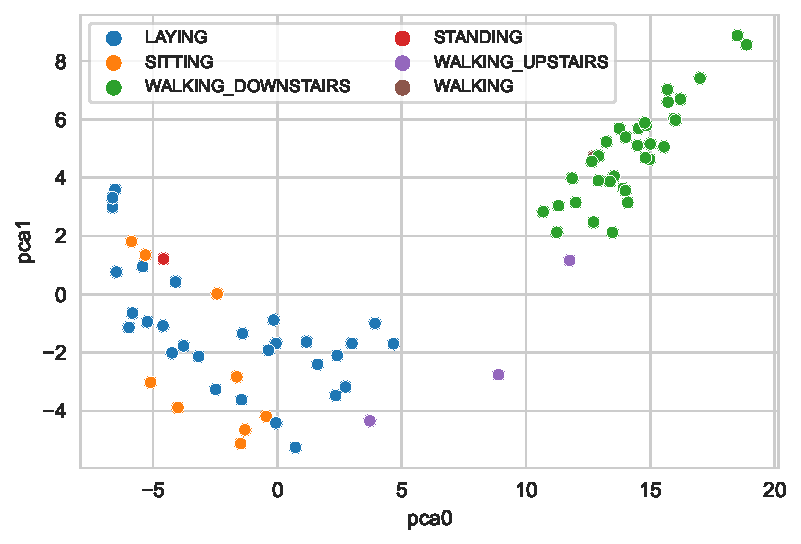
\includegraphics[width=\linewidth]{immagini Lia/all_classes_anomalies.pdf}
    \caption{Anomalies in the class.}
    \label{fig:ana}
  \end{subfigure}
  \hfill%%
  \begin{subfigure}[t]{0.49\columnwidth}
    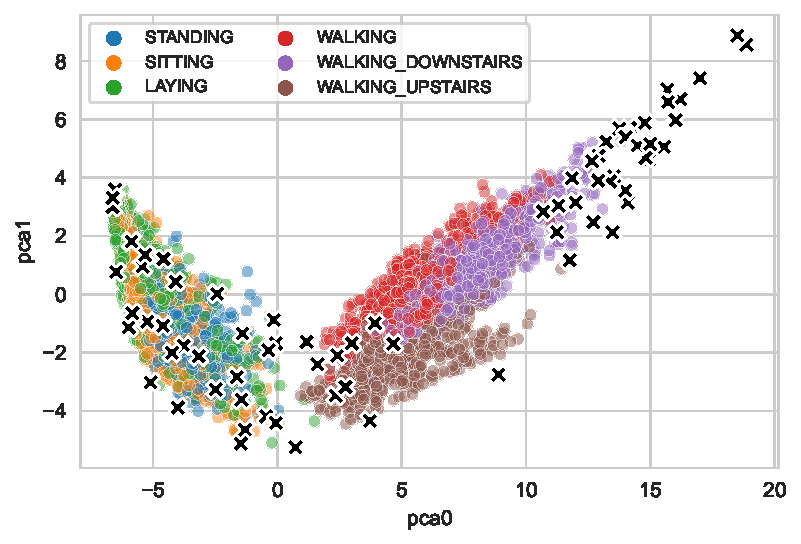
\includegraphics[width=\linewidth]{immagini Lia/anamoalies_of_the_class.pdf}
    \caption{Distribution of all anomalies.}
    \label{fig:allclassesana}
  \end{subfigure}
\caption{Scatter plot showing the distribution of outliers in the dataset.}
\label{fig:majority}
\end{figure}

\begin{table}[h]
    \centering
    \caption{Outliers detected with various techniques.}
    \begin{tabular}{lr|lr|lr}
        \toprule
        DBSCAN & 69 & IF & 74 & Likelihood & 13 \\
        LOF & 74 & EIF & 54  & Mahalanobis & 4 \\
        KNN & 73 & Grubbs & 2 & Depth-Based & 14 \\
        ABOD & 73 &  &  &  & \\
        \bottomrule
    \end{tabular}
    \label{tab:outliers}
\end{table}

\subsection{Dimensionality Reduction}

In order to reduce the dimensionality of the engineered dataset, we used three different feature selection approaches approaches. However, these techniques are computationally expensive, thus, due to the high number of variables, we first performed a preprocessing step that allowed us to speed up the procedure. 

Specifically, we run the decision tree alone to detect the attributes that were never used during the tree construction procedure and remove them from the set of features. 

This strategy allowed us to discard 413 attributes out of the initial 540. Hence, we applied the dimensionality reduction techniques only to a dataset composed of 127 variables.

In addition to this analysis, in the second part of this section, we also tested different feature extraction strategies like PCA, IsoMap, MDS, t-SNE. 

\subsubsection{Feature Selection}\label{subsec:feature_selection}

We will start with the filter approach and then continue the discussion with the embedding and wrapper techniques. 

\paragraph{Filter Strategy.}
In order to select the "optimal" set of features, we applied the filter strategy by combining the scikit-learn SelectKBest algorithm with a cross-validation approach. Namely, we evaluated all the $K$ best attributes (from $K = 1$ to $K = 127$) according to different external score functions.

The SelectKBest algorithm with cross-validation removes one feature at a time without using an endogenous measure. This function assigns a score to each feature before the cross-validation procedure starts. 

The score functions we used with the filter strategy approach are the followings: variance threshold, F-test, eta-squared ($\eta^2$); Mutual Information (MI).

Unlike the other functions, the variance threshold does not consider the target variable to compute the scores. The idea is that attributes with the greatest variance potentially have a greater ability to predict the dependent variable. 

The same reasoning applies with the other three measures, except that, in order to be computed, they also takes information from the target variable and thus can be considered supervised methods. For F-test and MI functions we used the built-in implementations of the scikit-learn library. Instead, the $\eta^2$ function was implemented from scratch. We used this measure since it is particularly suitable for measuring the dependencies among quantitative and categorical variables. Specifically, we used the following formula $\eta^2_{X|Y} = \frac{\sigma^2_{\mathrm{Mean}(X|Y)}}{\sigma^2_X}$, where $\mathrm{Mean}(X|Y)=\mu_{X|Y=y_i}$ are the conditional means.

\begin{figure}
    \centering
    \begin{subfigure}[t]{0.49\linewidth}
        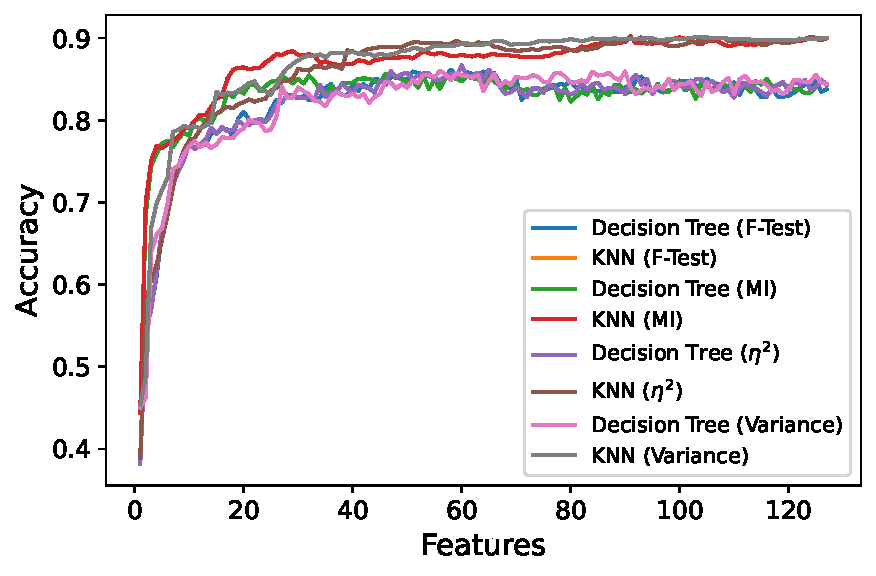
\includegraphics[width=\linewidth]{immagini simone/output_214_0.pdf}
        \caption{Filter strategy.}
        \label{fig:filter}
    \end{subfigure}
    \hfill%%
    \begin{subfigure}[t]{0.49\columnwidth}
        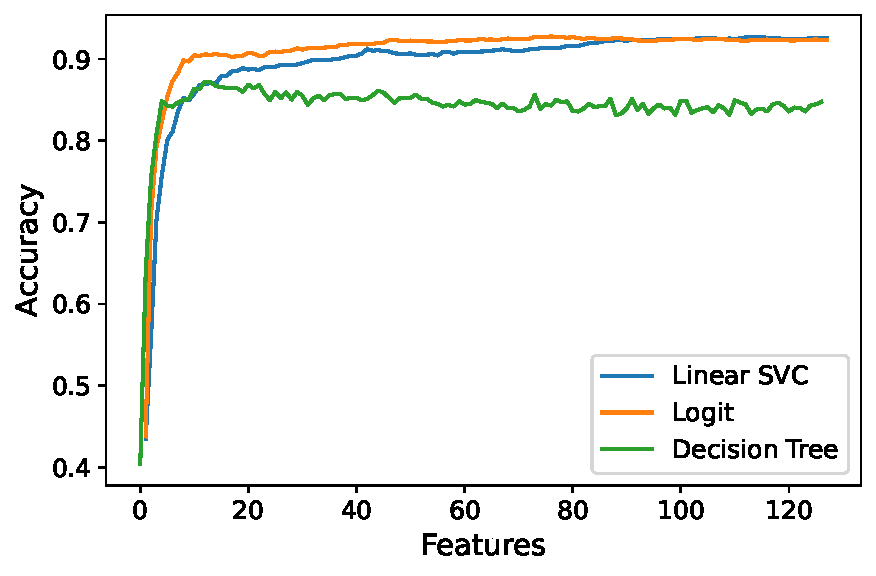
\includegraphics[width=\linewidth]{immagini simone/output_118_0.pdf}
        \caption{Embedded strategy.}
        \label{fig:embedded}
    \end{subfigure}
    \caption{Dimensionality reduction: filter and embedded approaches.}
\end{figure}

We tried the SelectKBest algorithm with all the score functions just presented, using both KNN and decision tree classifiers. The results are depicted in Figure \ref{fig:filter}. As one can see, in the range $[1,40]$ the Mutual Information approach seems to select the best features with respect to both classifiers. Probably, this depends on the fact that MI can capture any kind of statistical dependence. For what concerns the KNN, $\eta^2$ and F-test seem to choose, approximately, the best features in the range $[40, 65]$ (orange and brown lines overlap). From 65 on, all the score functions seem to behave in the same manner.

\paragraph{Embedding strategy.}
We applied the embedded strategy using the scikit-learn Recursive Feature Elimination with Cross-Validation (RFECV) function.

The procedure is the following: initially, the estimator is trained on the set containing the 127 best attributes. At each iteration, the least important attribute is removed from the set. The usefulness of each variable is measured with respect to its coefficient or its feature importance (that is, the measure "embedded" in the classifier). Moreover, at each iteration we keep track of the accuracy of the classifier and in the end we select the subset of features that produced the highest accuracy. 

We adopted this strategy with three different classifiers: Decision Tree, LinearSVC and Logistic regression. Figure \ref{fig:embedded} depicts that, despite the model used, accuracy enhances steeply in the range $[1,20]$, and then it becomes almost steady. Actually, for the decision tree classifier, it even decreases after the 23 selected best features. By running the Logit and LinearSVC estimators with the best 23 features selected with the decision tree classifier, only entails a small accuracy drop of about 3\% with respect to the accuracy obtained by using their best attributes. Moreover, by comparing filter and embedded strategies considering only the decision tree (see Figure~\ref{fig:filter_vs_embedded}), it is evident that the second approach result in better performances (accuracy increases faster).

\begin{figure}
    \centering
    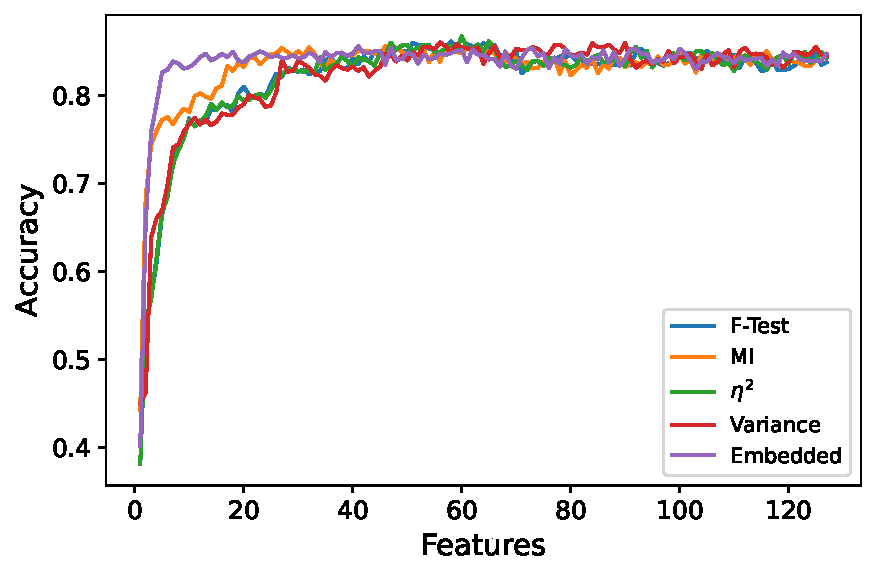
\includegraphics[width=0.667\linewidth]{immagini simone/output_219_0.pdf}
    \caption{Filter vs embedded approach with the decision tree classifier.}
    \label{fig:filter_vs_embedded}
\end{figure}

\paragraph{Wrapper strategy.}
With respect to the previous analysis, it is important to notice that the order by which the classifiers eliminate the features is probably not the same for all classifiers. Furthermore, this strategy only search in a small portion of the space of all possible combinations of attributes. Therefore, in order to enhance our choice, we conducted a further analysis. In particular, we used the wrapper approach. 

We set aside the set of the best 23 features selected from the decision tree with the embedded strategy. Let's call it A. Then, we combined the best 25 features selected by the other classifiers (for both approaches, filter and embedded). Let's call this set B. Then, we iterated over the latter set and, for each variable, added it to A (if not already present) and performed a new classification with the decision tree. If the accuracy did not increase, we removed the appended features and continue to iterate over B until we performed an entire cycle (epoch) without adding any new attribute in the set A. However, no features were able to improve the current accuracy. 

In conclusion, given the just explained reasons and even to make the analyses which will be conducted in the next sections harder, we decided to reduce the dimensionality of the dataset by taking only the set of the best 23 attributes selected by the decision tree using the embedded strategy. Due to the length of the names of the selected 23 variables, we decided to report only their indices, as shown in the \textit{features.txt} file: 38, 41, 51, 52, 53, 54, 55, 58, 68, 72, 75, 77, 130, 133, 160, 210, 303, 394, 449, 451, 504, 509, 560.

\subsubsection{Feature Extraction}

Along with feature selection techniques, we also try out feature extraction strategies. We tested linear and non-linear transformations, for both visualization and classification purposes Namely, we used: principal component analysis (PCA), IsoMap, Multidimensional Scaling (MDS) and t-SNE.

For every technique, we plotted the decision boundaries of both the decision tree and KNN classifiers in a 2D reduced space. For space economy, we decided to show only the non-linear decision boundaries produced by the KNN. By doing so, it is also possible to appreciate the difference between the different approaches.

\begin{figure}
\centering
    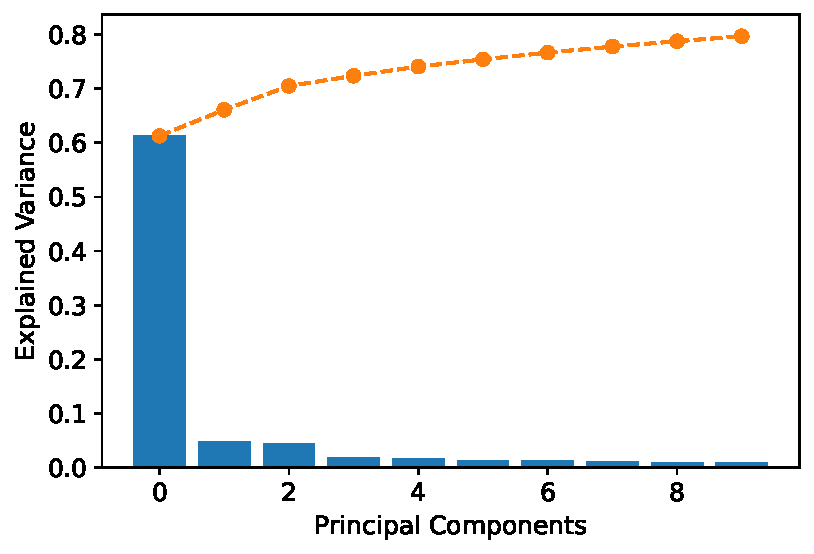
\includegraphics[width=.64\linewidth]{immagini simone/pca_explained_var.pdf}
    \caption{Individual (in blue) and cumulative (in orange) explained variance for the first 10 principal components.}
    \label{fig:expca}
\end{figure}

\paragraph{PCA} is a linear dimensionality reduction technique. As shown in Figure \ref{fig:expca}, the first component explains more than 63\% of the variance of all 561 variables. However, all other components explain a very small percentage of the residual variance. To achieve a significant explained variance we need to use more than 11 components.
    
We performed a cross-validation to tune the optimal number of components, searching them within the range $[1,50]$. In the pipeline, we used both decision tree and KNN, but without tuning their hyperparameters. On the PCA latent space, the classifiers reached the maximum accuracy with 24 principal components, where the cumulative explained variance was 86.76\%. 
    
Specifically, the decision tree obtained an accuracy of 78\%, whereas the KNN 87\%. For both models this scores were biased due to a very high F1 statistic on the LAYING class~(96\%-98\%). In fact, the overall performances on the other classes were significantly lower.

On the other hand, by using only the first two principal components, for both models the accuracy reached was very poor: 55.11\% for the KNN and 51.5\% for the decision tree. Figure~\ref{fig:pca_db} depicts the decision boundaries produced by the KNN classifier on the2D dataset.  

\paragraph{IsoMap} is a non-linear dimensionality reduction through Isometric Mapping. For visualization purposes, we tried to plot the reduced dataset trying to select the best number of neighbors, however this parameter does not make much difference.

Here too, we tried to tune the best number of components. The grid search resulted in 7 components with an accuracy of 81\% for the decision tree and 84\% for KNN. Also in this case, the results were biased by an F1 score close to 100\%. On a 2D isomap space the classifiers behaved better with respect to PCA. The decision tree reached an accuracy of 67.44\%, while the KNN of 72.46\%. Figure~\ref{fig:isomap_db} shows the KNN decision boundaries in this space. 

\begin{figure}[t]
    \centering
    \begin{subfigure}[t]{0.49\linewidth}
        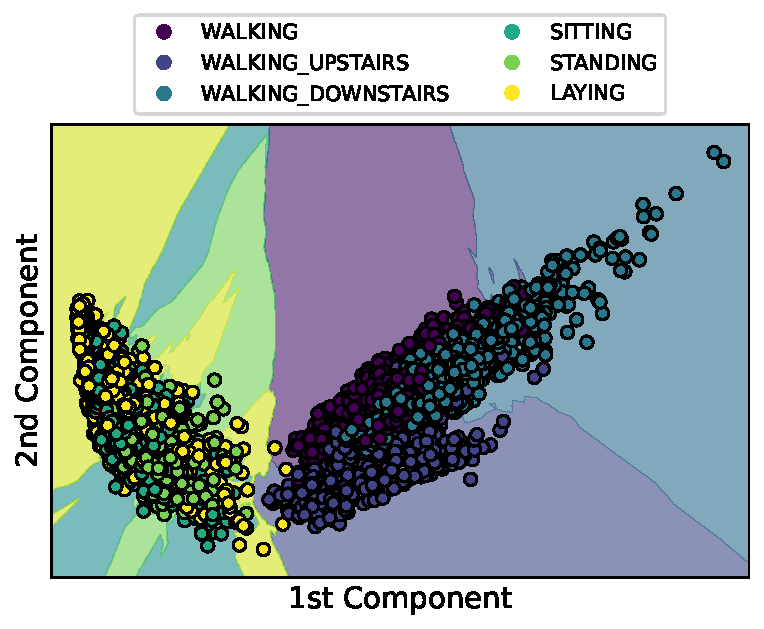
\includegraphics[width=\linewidth]{immagini simone/PCA_KNN_decision_boundaries.pdf}
        \caption{PCA}
        \label{fig:pca_db}
    \end{subfigure}
    \hfill%%
    \begin{subfigure}[t]{0.49\linewidth}
        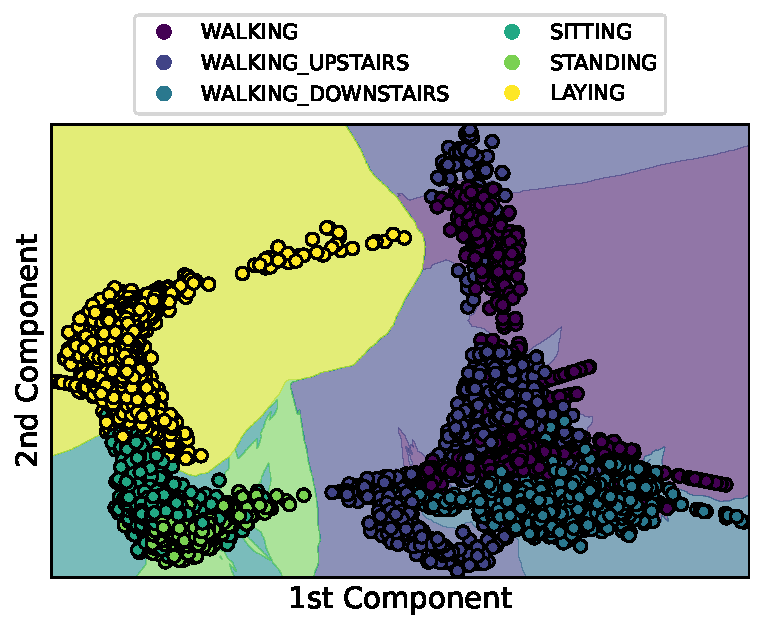
\includegraphics[width=\linewidth]{immagini simone/KNN_decision_boundaries_isomap.pdf}
        \caption{IsoMap}
        \label{fig:isomap_db}
    \end{subfigure}    
\vskip\baselineskip
    \begin{subfigure}[t]{0.49\linewidth}
        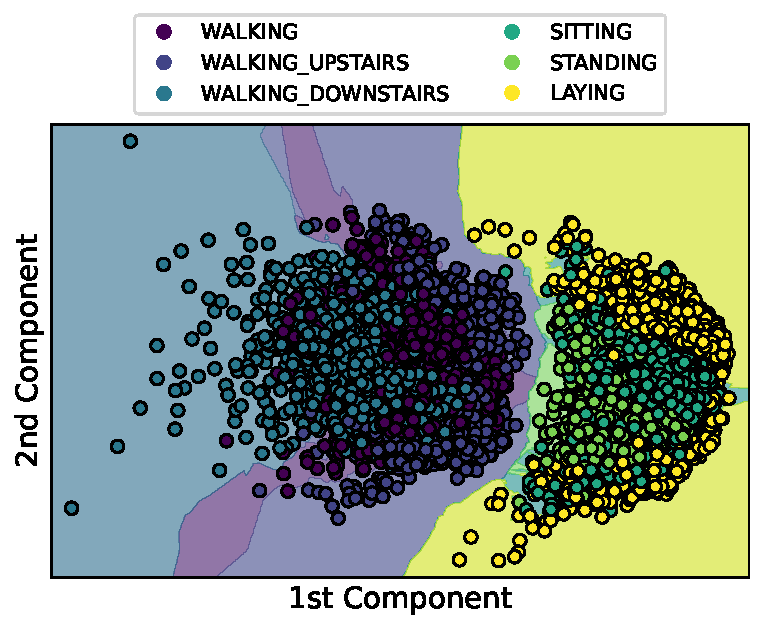
\includegraphics[width=\linewidth]{immagini simone/KNN_decision_boundaries_MDS.pdf}
        \caption{MDS}
        \label{fig:mds_db}
    \end{subfigure}
    \hfill%%
    \begin{subfigure}[t]{0.49\columnwidth}
        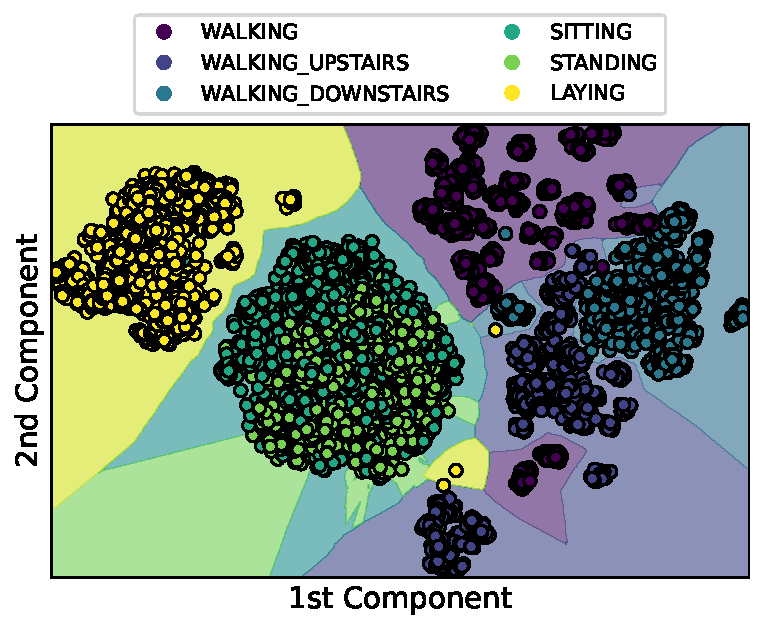
\includegraphics[width=\linewidth]{immagini simone/KNN_decision_boundaries_tsne.pdf}
        \caption{t-SNE}
        \label{fig:tsne_db}
    \end{subfigure}
\caption{KNN decision boundaries: a comparison among all the features extraction techniques.}
\label{fig:latent_spaces}
\end{figure}

\paragraph{MDS} is a manifold learning technique that can be thought of as an attempt to generalize PCA to capture non-linear structure in the data. 

In the scikit-learn library, the MDS and t-SNE functions do not have the transform method. They can be used only for visualization purposes because, as reported in the library documentation, they are transductive learners. 

To be consistent with the analyses previously conducted for PCA and Isomap, and just for didactic purposes, we tried to replicate the same analysis following the steps below: %
%
\begin{enumerate*}
    \item	join the train and test set;
    \item	compute the latent space with MDS;
    \item	separate again the dataset in train and test sets;
    \item	train the classifier on the train set;
    \item	test the classifier on the test set.
\end{enumerate*}

Due to the slowness of the algorithm, to find the optimal number of components, we analyzed a 10\% stratified random sample. The highest accuracy was reached with 3 components. However, the performances did not appear to be very sensitive to the number of components used. 

By training the classifiers on the whole 3D reduced dataset, we obtained higher performances than PCA and Isomap. This is probably because when we reduced the dimensionality of the dataset, we also used the information on the test set. Hence, the classifiers were not tested on "new unseen data". Specifically, the decision tree and KNN obtained an accuracy of, respectively, 70\% and 75\%. Again the LAYING class obtained a very high F1 score (99\%).

Figure~\ref{fig:mds_db} shows the KNN decision boundaries in a 2D space. Here, the accuracy for both classifiers were ranging from 61\% to 64\%. 

\paragraph{t-SNE} is a transductive learner used for visualization purposes. As reported in the official documentation, due to the Barnes-Hut approximation, the maximum number of components the scikit-learn implementation can use is 3. 

We reached a higher accuracy using 2 components. Specifically, the decision tree reached an accuracy of 87\%, while the KNN had an accuracy of 91\%. Like MDS, since we computed the embedded features considering the test set too, the results suffer from overfitting. Again the LAYING class was always correctly predicted.

As for the other techniques, we reported the decision boundaries in the 2D space shown in Figure~\ref{fig:tsne_db}. To reproduce the figure we tested different parameters. Specifically, we used a PCA initialization and set the learning rate to "auto", but we tested all the perplexity values in the set $\{10,20,30,40,50\}$. Eventually, we decided to set the perplexity parameter at 50, as the classes seem to be better separated.

Figure~\ref{fig:comparison_fe} shows a final comparison among all the features extraction techniques discussed in this subsection.

\begin{figure}
\centering
    \begin{subfigure}[t]{0.49\linewidth}
        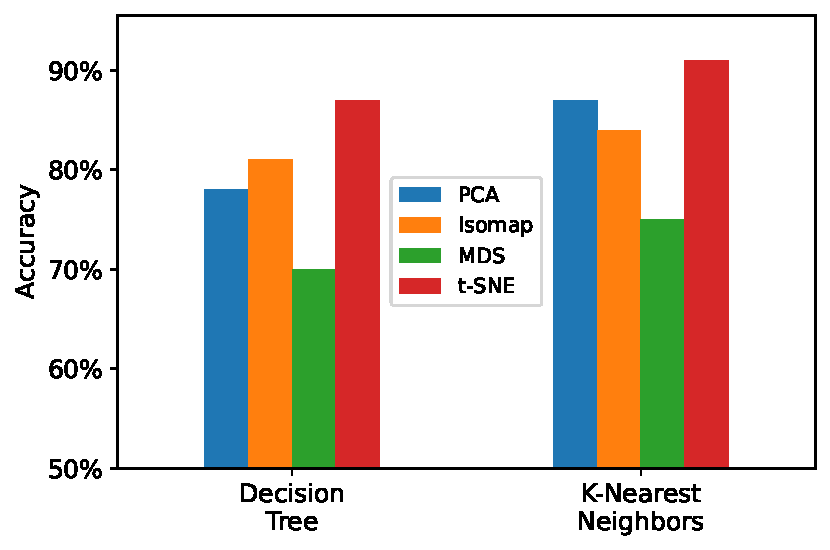
\includegraphics[width=\linewidth]{immagini simone/fe_comparisons.pdf}
    \end{subfigure}
    \hfill%%
    \begin{subfigure}[t]{0.49\columnwidth}
        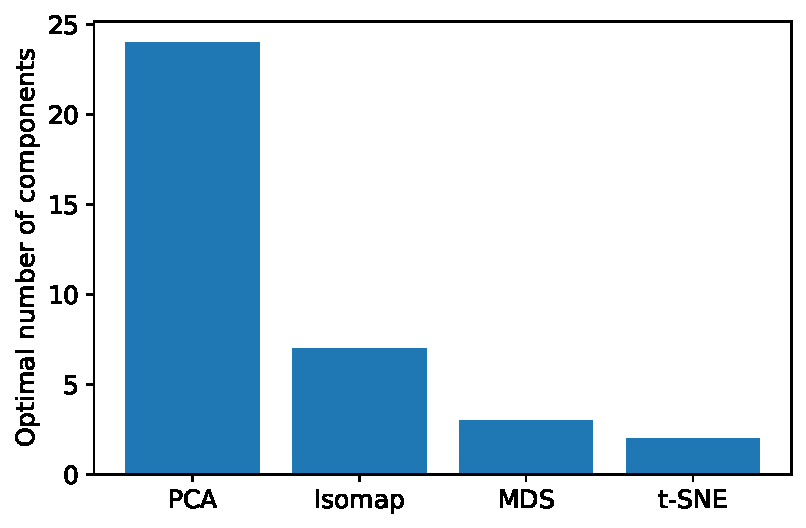
\includegraphics[width=\linewidth]{immagini simone/fe_n_components.pdf}
    \end{subfigure}
\caption{Comparison among feature extraction approaches.}
\label{fig:comparison_fe}
\end{figure}

\subsection{Imbalanced Learning}\label{sec:imbalancedlearning}

To conform to the project guidelines, now we are going to present the imbalance learning analysis. As observed in subsection~\ref{subsec:data_understanding}, the different classes have approximately the same cardinality, thus the first step was to unbalance the dataset. Specifically, we considered two different strategies:
%
\begin{enumerate}
\item Relabel the activities in movement and stationary activities, unbalance one of them, end perform binary classification;\label{enum:stat_vs_dynamic}
\item Select two classes, unbalance one of them, and perform a binary classification;\label{enum:wup_vs_wdown}
\end{enumerate}
%
In all three cases, we decided to apply a very aggressive unbalance rate that produced a dataset composed of 96\% from the majority class and 4\% from the minority class. The dataset we are referring to is the one without the 78 outliers and with the best 23 filter selected features as discussed previously.

With respect to point~\ref{enum:stat_vs_dynamic}, there is not much to say. All the latent spaces in Figure~\ref{fig:latent_spaces} show that dynamic and stationary activities are well separated and thus very different from each other. As a result, all the classifiers used achieved 100\% accuracy without even tuning the hyperparameters or applying some imbalance technique.

As regards the point~\ref{enum:wup_vs_wdown}, we decided to work only on the WALKING UPSTAIRS and WALKING DOWNSTAIRS classes. Indeed, by looking at the scatter plots in Figure~\ref{fig:latent_spaces}, those two classes seemed to be the hardest to distinguish. However, as we will see in the next subsection, the activities most difficult to distinguish are SITTING and LAYING.

To perform this task we used both undersampling and oversampling techniques, as well as a combination of them. We chose to use only the decision tree classifier to compare the different imbalance approaches. Moreover, for each classification, we performed cross-validation to tune the classifier hyper-parameters. In general, we used 5 stratified folds, however, with the undersampling techniques that produced too small train sets, we opted for the Leave-One-Out strategy. To save space, we decided not to report the optimal parameters.

The decision tree trained on the unbalanced dataset performed pretty well, obtaining an accuracy of 82\%. However, as expected, the classifier was biased toward the negative class, thus predicting most of the time the majority class. Generally speaking, this pattern was also observed with all the imbalance techniques used. As a result, all of them are characterized by high precision and small recall (see Figure~\ref{fig:imb_comparison}).

Below we briefly describe the algorithms used:
%
\begin{description}
\item [Random undersampling] of the majority class until the classes reach the same cardinality. 
\item [Condensed Nearest Neighbors] (CNN) to remove objects of the majority class that are not necessary to predict the positive class. 
\item [Random oversampling] of the minority class to duplicate each record in the dataset the same number of times until the imbalance between classes is compensated.
\item [SMOTE] to create artificial records by making convex linear combination between pairs of records of the minority class.
\item [Tomeklinks] is a lightweight undersampling technique that eliminates records of the majority class which are part of a Tomek's link. For our dataset this method did not find any Tomek's link and thus the results are the same obtained using the unbalanced dataset.
\item [Edited Nearest Neighbors] (ENN) undersampling technique that removes the object of the majority class which do not agree with their $k$ neighbors. Even this method did not have benefits with our dataset. Selecting a number of neighbors equal to 5 it removed only 9 records, whereas with 10 neighbors it removed 18 objects.
\item [SMOTETomek] a mixed technique that first performs an oversampling of the minority class using SMOTE and then cleans the dataset applying the TomekLinks undersampling of both classes. It did not find any Tomek's link after the SMOTE step. Therefore, it produces the same results of the plain SMOTE.
\item [SMOTEENN] like SMOTETomek, but instead of TomekLinks, it uses the ENN as undersampling technique. With 5 neighbors it performed better than the plain SMOTE. 
\item [ADASYN] an oversampling technique very similar to SMOTE. Instead to produce the same number of artificial records for each object of the positive class, the minority records that in their neighborhood have more objects belonging to the majority class (and thus are "harder-to-learn"), produce more artificial instances. We used 3 neighbors.
\item [Meta-cost sensitive] approach using the COSTCLA module. Namely, it is a decision tree classifier using a specified weighting schema. Since we were interested in predicting the positive class we put more weight on false-negative predictions. We tried different cost combinations, but in the end, we decided to report only the following: $\mathrm{FP}=1$, $\mathrm{FN}=10$, $\mathrm{TP}=0$, $\mathrm{TN}=0$.
\item [Class weight] parameter of the decision tree set to "balanced". In this way, the scikit-learn implementation of the decision tree automatically adjusts the weights inversely to the frequency of classes. With an accuracy score of 87\% and a recall equal to 78\% this was the best technique applied. 
\end{description}

All our analysis is summarized in Figures~\ref{fig:imb_curves} and~\ref{fig:imb_comparison}. Generally speaking, despite the large unbalancing between the two classes, this was not a challenging task for the decision tree. Indeed, without applying any technique it was able to obtain an accuracy of 82\%. Moreover, from Figure~\ref{fig:imblift} we can observe that every model is approximately two times better than the random choice for a large percentage of samples. In general, it seems that the oversampling approaches performed worst, especially due to their small recall. By looking at the ROC and the PR curves in Figures~\ref{fig:imbroc} and~\ref{fig:imbprerec}, the ADASYN algorithm shows a very large AUC, but oddly, its accuracy was modest. As depicted by its precision-recall curve, this may depend on a slighter (with respect to the other methods) trade-off between precision and recall for low threshold values.

\begin{figure}
    \centering
    \begin{subfigure}[t]{0.49\linewidth}
        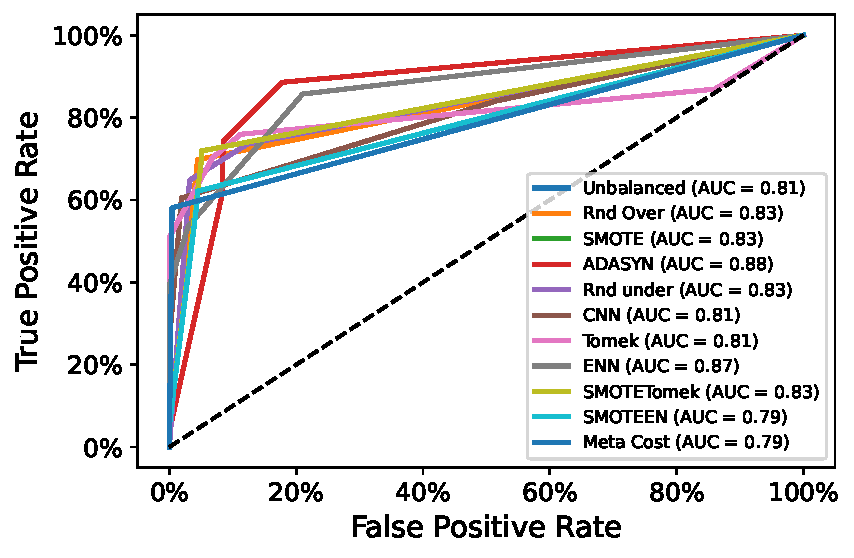
\includegraphics[width=\linewidth]{immagini simone/imb_roc_comparison.pdf}
        \caption{ROC}
        \label{fig:imbroc}
    \end{subfigure}
    \hfill%%
    \begin{subfigure}[t]{0.49\columnwidth}
        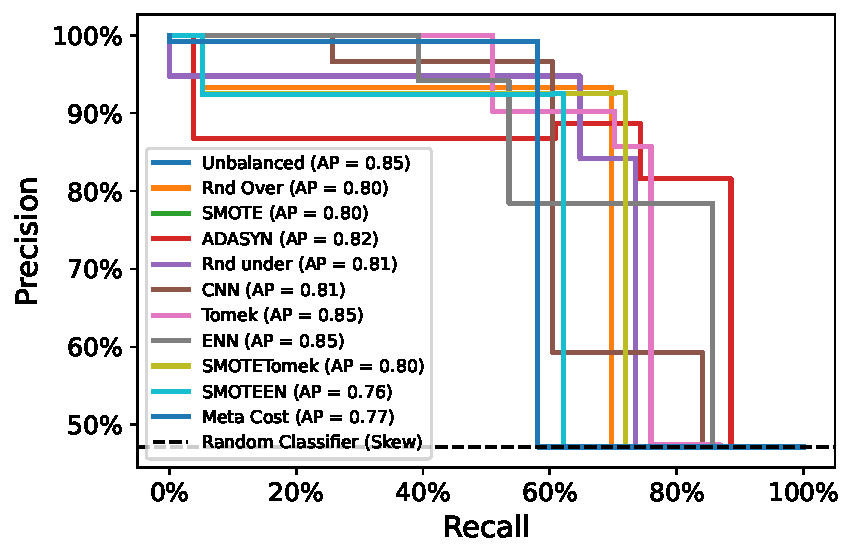
\includegraphics[width=\linewidth]{immagini simone/imb_pre_rec_comparison.pdf}
        \caption{Precision-Recall}
        \label{fig:imbprerec}
    \end{subfigure}
    \begin{subfigure}[t]{0.49\linewidth}
        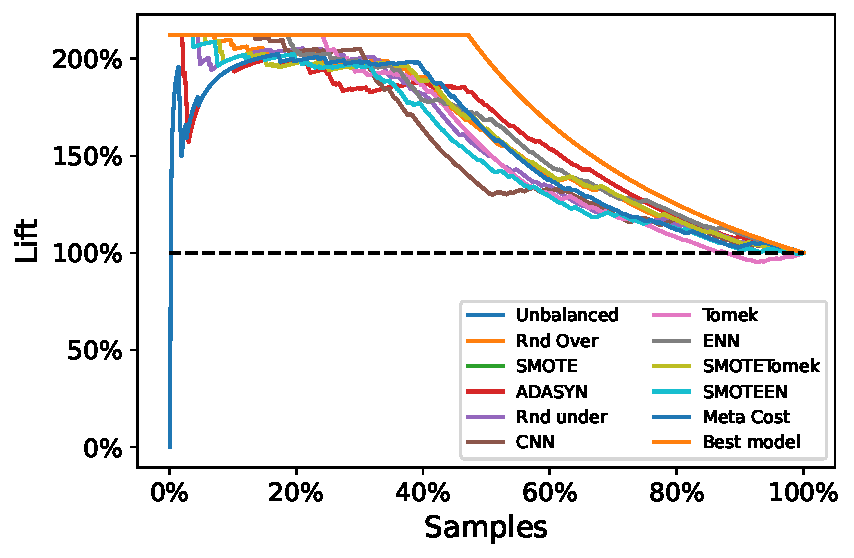
\includegraphics[width=\linewidth]{immagini simone/imb_lift_comparison.pdf}
        \caption{Lift Chart}
        \label{fig:imblift}
    \end{subfigure}
    \hfill%%
    \begin{subfigure}[t]{0.49\columnwidth}
        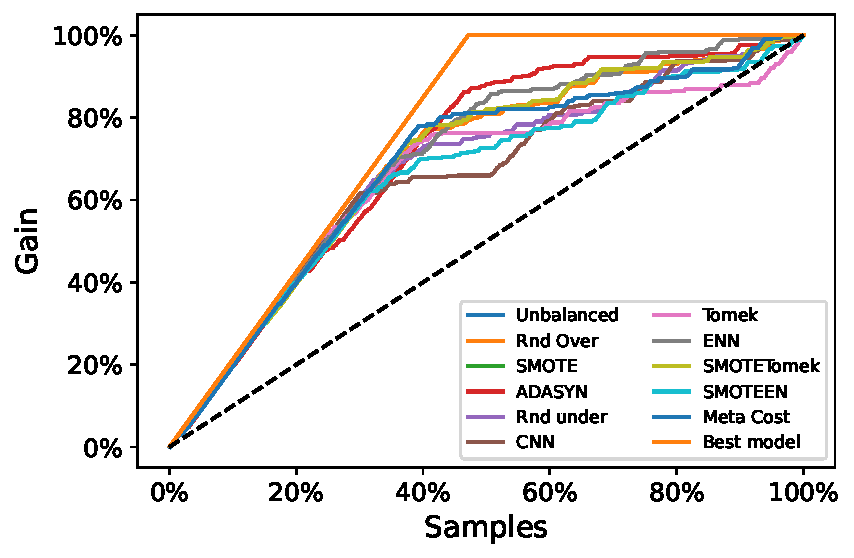
\includegraphics[width=\linewidth]{immagini simone/imb_gain_comparison.pdf}
        \caption{Gain Chart}
        \label{fig:imbgain}
    \end{subfigure}
    \caption{Evaluation curves for imbalance learning.}
    \label{fig:imb_curves}
\end{figure}

\begin{figure}
    \centering
    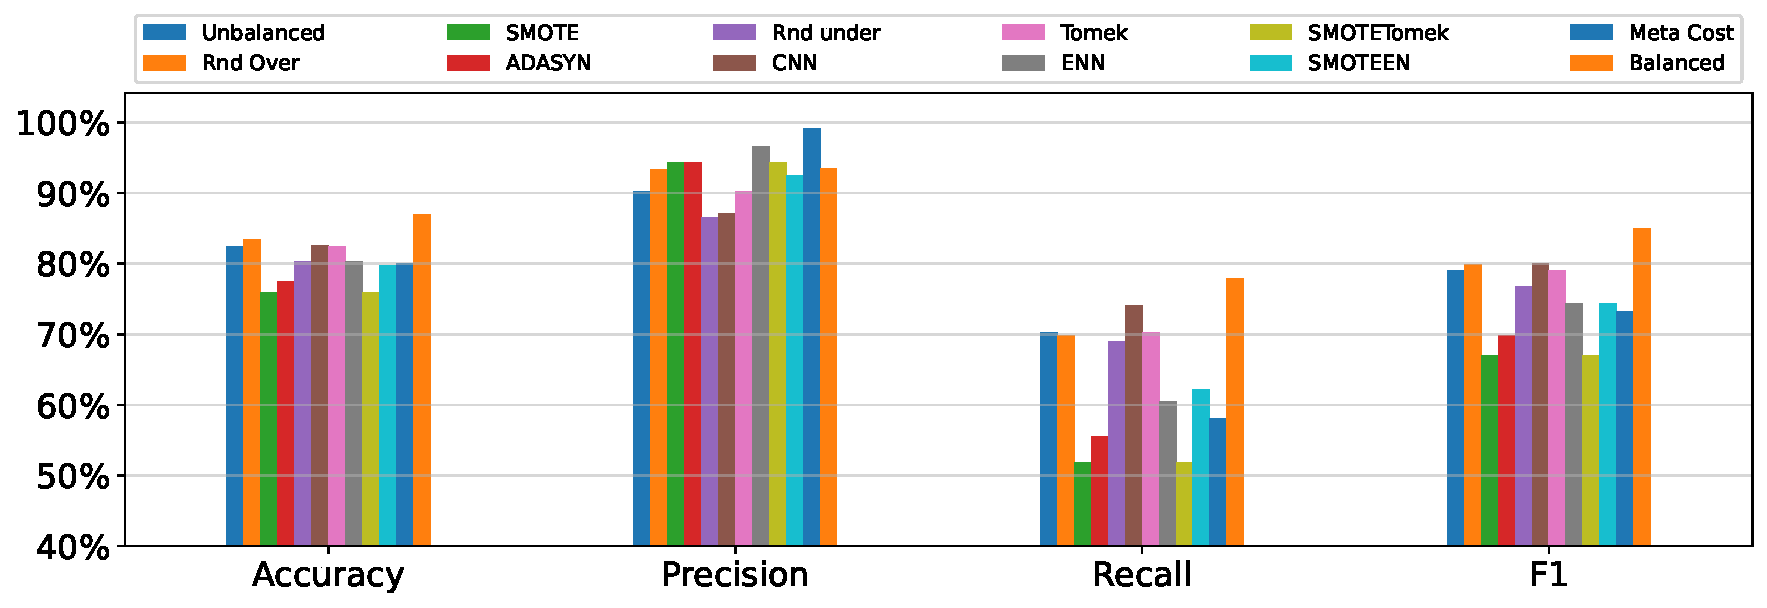
\includegraphics[width=\columnwidth]{immagini simone/imb_score_comparison.pdf}
    \caption{Model comparison among imbalance techniques. Apart from accuracy, which is a global measure, all other scores relate to the positive class.}
    \label{fig:imb_comparison}
\end{figure}

\subsection{Basic Classification Methods}

As prescribed by the project guidelines, we performed a preliminary multiclass classification using the KNN and decision tree classifiers. 

As noted earlier, since the LAYING class is almost always correctly predicted, we decided to remove it from the dataset to make the classification more challenging. Therefore, the results we are going to present here and in the subsequent sections are obtained using the five residual classes on the dataset composed of the 23 best features selected in subsection \ref{subsec:feature_selection}.

For both classifiers, we performed a hyperparameters search using a 5-fold cross-validation. Specifically, the search space we used to tune the decision tree parameters was: maximum depth in the integer interval $1,2,\dots,10$; minimum number of samples per leaf in $\{25, 30,\dots, 60\}$; and maximum number of leaves in $\{10, 15,\dots, 50\}$. Instead, for the KNN we used: a number of neighbors in the following interval composed of odds integers $\{1,3,\dots,21\}$; uniform and distance based weights; and the three principal metrics---Manhattan, Euclidean, Chebyshev.

The optimal decision tree had 5 levels, a maximum of 20 leaves, and a minimum number of samples per leaf equal to 35. On the other hand, the best KNN model utilized the Manhattan distance, 11 neighbors, and an uniform weight.

The decision tree obtained an accuracy of 81\%, but struggled to distinguish correctly between WALKING UPSTAIRS and WALKING DOWNSTAIRS classes. Indeed, the F1 score were, respectively, 76\% and 77\%. On the contrary, it managed to predict the WALKING class very well, obtaining a F1 score of 98\%. Instead, the harmonic mean of precision and recall for the SITTING and STANDING classes were, respectively, 80\% and 84\%.

On the other hand, the KNN got a total accuracy of 86\% and, in general, behaved well on both static classes dynamic classes, although the performances on the latter were significantly better.

This trend was observed for all the classifiers used in this project, both those trained and tested on the dataset with the engineered features and, as we shall see later, on the time series dataset. This is due to low recall on the SITTING class and low precision on the STANDING class. In the former case, this means that when objects belonging to the SITTING class are presented, classifiers struggle to distinguish them from those belonging to the STANDING class. In the second case, however, it means that the percentage of times that classifiers guess when predicting the STANDING class tends to be lower. In this case, this is evident by looking at the confusion matrix in the figure~\ref{fig:comparison_confusion}. Furthermore, it can also be seen that almost never an object belonging to one of the dynamic classes is predicted with one of the static classes, and vice versa.

\begin{figure}
\centering
    \begin{subfigure}[t]{0.40\linewidth}
        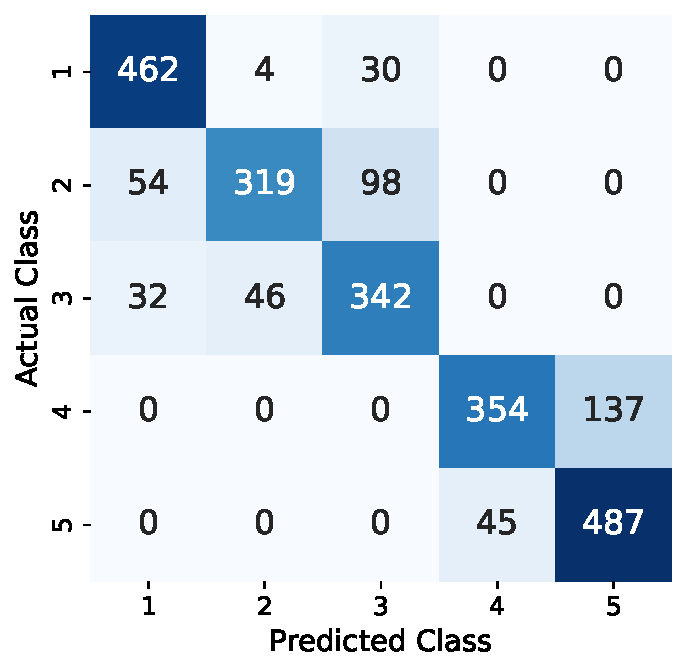
\includegraphics[width=\linewidth]{immagini simone/dtc_tuned_conf_mtx.pdf}
        \caption{Decision Tree}
        \label{fig:dtroc}
    \end{subfigure}
    %\hfill%%
    \hspace{0.4cm}
    \begin{subfigure}[t]{0.40\columnwidth}
        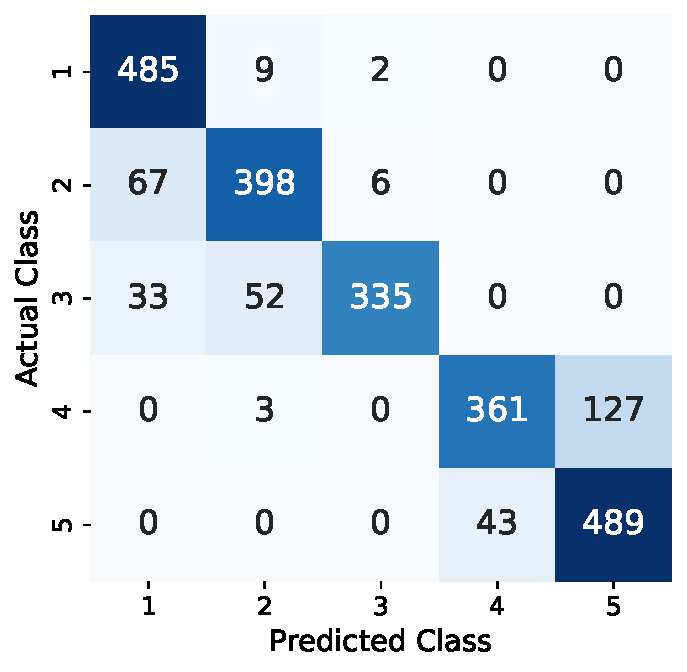
\includegraphics[width=\linewidth]{immagini simone/knn_tuned_conf_mtx.pdf}
        \caption{KNN}
        \label{fig:knnroc}
    \end{subfigure}
\caption{Decision tree and KNN confusion matrices.}\label{fig:comparison_confusion}
\end{figure}

\subsection{Conclusions}\label{subsec:module1_conclusion}

Before to go ahead, we briefly summarize the results of the analyses conducted in this section. 

We first removed 21 duplicate variables. Next, we performed an outlier analysis that allowed us to identify and remove 78 outliers from the train set. Next, we evaluated several dimensionality reduction techniques. We chose to keep only the best 23 attributes selected from the decision tree using the embedded approach. Finally, looking at the results of the first plain classifications, we noticed that the LAYING class was being predicted with the highest accuracy, so we decided to remove the objects belonging to that class from both the training and test sets.

Therefore, the data sets we will use in the second section of this project have the following shapes: $5896 \times 23$ for the train set and $2410 \times 23$ for the test set.

\section{Advanced Classification Methods}

In this section, we will first discuss some of the most advanced classification techniques and present the results obtained using the dataset summarized in subsection~\ref{subsec:module1_conclusion}. Then we will use the same models to deal with the regression task. 

Specifically, we will cover the following models or families of models: naive Bayes, logistic regression, support-vector machines, neural networks and ensemble methods. In the latter case, we will discuss both averaging (random forest) and boosting methods (AdaBoost, GradientBoostingClassifier, XGBoost, LightGBM).

\subsection{Classification}

\subsubsection*{Naive Bayes Classifier}

In this subsection, we discuss the results obtained with the Naïve Bayes classifier for multi-class problem.

We trained the model on various datasets. First, with the dataset consisting of the 23 features, we attempted to classify records into six classes:
%
\begin{enumerate*}
    \item WALKING,
    \item WALKING UPSTAIRS,
    \item WALKING DOWNSTAIRS,
    \item SITTING, 
    \item STANDING,
    \item LAYING.
\end{enumerate*}
%
Taking into account the class Laying, as shown in Table \ref{tab:naivebayes}, we noticed that the accuracy value is slightly higher (85\%) than when the latter is not considered (82\%). 

\begin{table}
\centering
\caption{Classification Report for Naive Bayes Classifiers. In the Table are shown the performance for the restricted and complete dataset.}
\label{tab:naivebayes}
\resizebox{\columnwidth}{!}{%
\begin{tabular}{|l|ccc|llc|l}
\cline{1-7}
\textbf{}                                                               & \multicolumn{3}{l|}{\textbf{Dataset with 23 features}}                                       & \multicolumn{3}{l|}{\textbf{Dataset with 540 features}}                      \\ \cline{1-7}
\textbf{}                                                               & \multicolumn{1}{c|}{\textbf{Precision}} & \multicolumn{1}{c|}{\textbf{Recall}} & \textbf{F1} & \multicolumn{1}{c|}{\textbf{Precision}} & \multicolumn{1}{c|}{\textbf{Recall}} & \textbf{F1}  \\ \cline{1-7} 
WALKING                                                       & \multicolumn{1}{c|}{0.83}               & \multicolumn{1}{c|}{0.96}            & 0.89        & \multicolumn{1}{c|}{0.85}               & \multicolumn{1}{c|}{0.82}            & 0.83     \\ 
\begin{tabular}[c]{@{}l@{}}WALKING UPSTAIRS\end{tabular}  & \multicolumn{1}{c|}{0.85}               & \multicolumn{1}{c|}{0.82}            & 0.83        & \multicolumn{1}{c|}{0.76}               & \multicolumn{1}{c|}{0.96}            & 0.84    \\ 
\begin{tabular}[c]{@{}l@{}}WALKING DOWNSTAIRS
\end{tabular} & \multicolumn{1}{c|}{0.90}               & \multicolumn{1}{c|}{0.81}            & 0.86        & \multicolumn{1}{c|}{0.83}               & \multicolumn{1}{c|}{0.83}            & 0.74      \\ 
SITTING                                                       & \multicolumn{1}{c|}{0.91}               & \multicolumn{1}{c|}{0.58}            & 0.70        & \multicolumn{1}{c|}{0.71}               & \multicolumn{1}{c|}{0.70}            & 0.78     \\ 
STANDING                                                      & \multicolumn{1}{c|}{0.71}               & \multicolumn{1}{c|}{0.93}            & 0.80        & \multicolumn{1}{c|}{0.85}               & \multicolumn{1}{c|}{0.72}            & 0.72  \\ 
LAYING                                                       & \multicolumn{1}{c|}{1.00}               & \multicolumn{1}{c|}{1.00}            & 1.00        & \multicolumn{1}{c|}{1.00}               & \multicolumn{1}{c|}{1.00}            & 0.99    \\ \cline{1-7}
\textbf{Accuracy}                                                       & \multicolumn{3}{c|}{85.27\%}                                                                 & \multicolumn{3}{c|}{82.21\%}                                             \\ \cline{1-7}
\end{tabular}%
}

\end{table}


In both cases, the performance of the classes is very high, ranging from 70\% to 96\%. The class SITTING, in both classification with and without class LAYING, shows a recall of 58\%, in fact as can be seen from the confusion matrix in Figure \ref{fig:conmat23}, 203 out of 493 records are predicted as a STANDING activity. Since the activities are very similar but performed in opposite ways, the model probably confuses the activities due to a slight shift or rotation of the device. Axis are not the same for average.

\begin{figure}
    \centering
    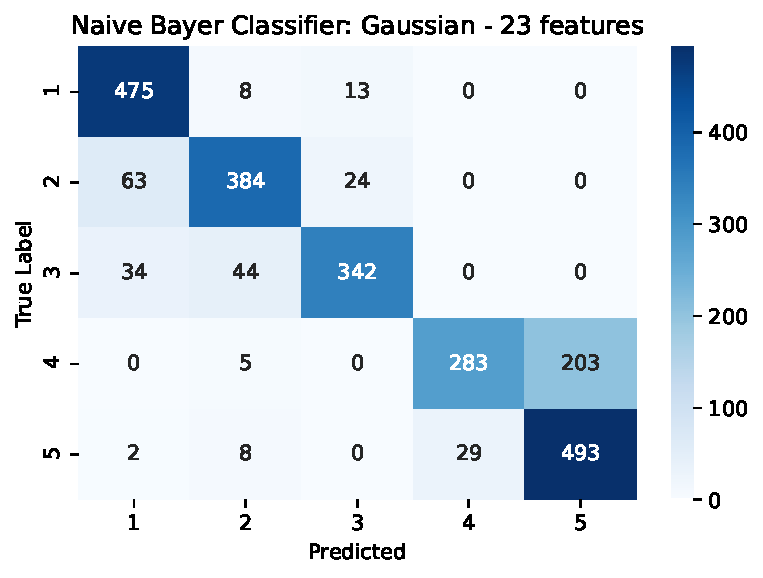
\includegraphics[width=0.5\linewidth]{immagini Lia/confusion_matrix_23_w6.pdf}
    \caption{Confusion matrix of the Naive Bayes Classifier with the dataset of 23 features without considering class LAYING.}
    \label{fig:conmat23}
\end{figure}

Although the other classes have high measures, some of them are predicted incorrectly, such as the class WALKING UPSTAIRS of which 384 records are predicted correctly, while the model predicts the remaining 63 as WALKING and the other 24 as WALKING\_DOWNSTAIRS. This could also be due to a problem with the motion sensors, which perceive a similar acceleration in both activities during the movement phase. The difference in predictions for the other classes is very slight. Optimal performance can also be seen from the ROC curves and precision and recall curves in Figure \ref{fig:dtc23}.



\begin{figure}

    \centering
    \begin{subfigure}[t]{0.48\columnwidth}
    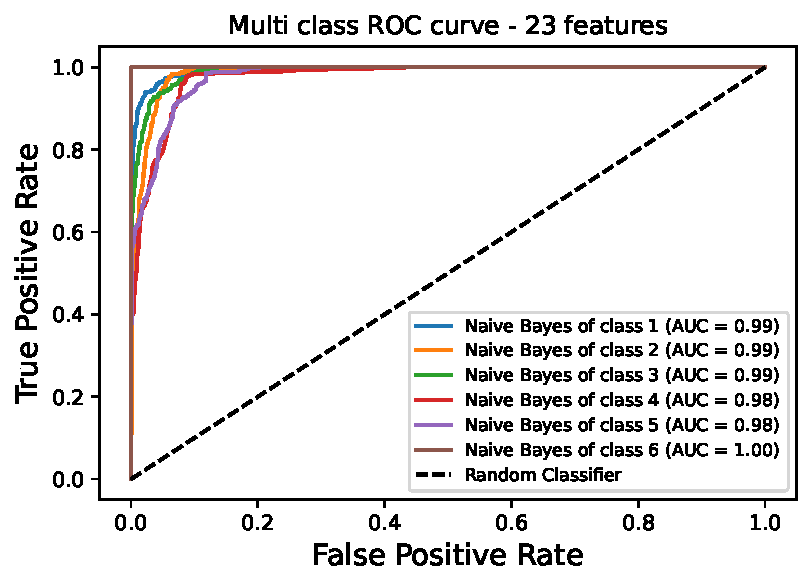
\includegraphics[width=\linewidth]{immagini Lia/dtc_multiclass_roc_23_features.pdf}
    \caption{ROC Curve}
    \label{fig:rocdt23}
\end{subfigure}
  \hfill %%
\begin{subfigure}[t]{0.49\columnwidth}
    \centering
    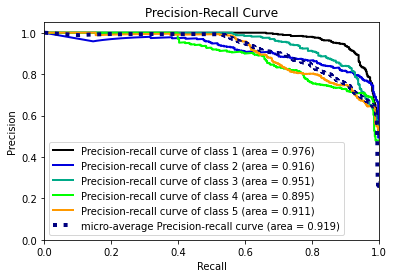
\includegraphics[width=\linewidth]{immagini Lia/download.png}
    \caption{Precision-Recall Curve}
    \label{fig:prerecdt}
    \end{subfigure}
    
    \caption{Graphs showing the results of the Naive Bayes Classifier using 23 features.}\label{fig:dtc23}
    
\end{figure}

The figure shows the ROC curves \ref{fig:rocdt23} for all classes (including class LAYING), which immediately show an increasing trend, a sign of positive prediction, and an area under the curve between a value of 0.97 and 0.99. From the graph of the precision and recall of the classes \ref{fig:prerecdt} without LAYING class, a slight difference can be seen for class 4 which for high precision values, starts to decrease when the recall takes on values greater than 0.4. Nonetheless, the value of the area under the curve is high, as can be seen also for the other classes.

The classifier was then trained on the entire dataset consisting of 540 features, testing also in this case the performance with and without the LAYING class. In all the analyses, the performances without class 6 are the same, except for accuracy. For the analysis with the 540 features and class LAYING included, the accuracy is 82\% (as with the 23 features), without class 6 it is 79\%. In contrast to the previous case both the classes WALKING DOWNSTAIRS and STANDING have a low recall of 67\% and 63\% respectively. 

\begin{figure}

    \centering
    \begin{subfigure}[t]{0.45\columnwidth}
    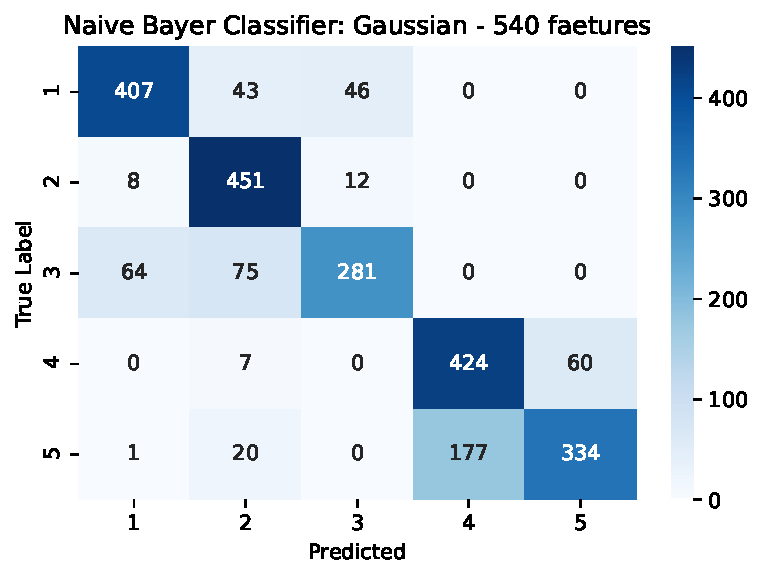
\includegraphics[width=\linewidth]{immagini Lia/confusion_matrix_540_w6.pdf}
    \caption{Confusion Matrix}
    \label{fig:conmat540}
\end{subfigure}
  \hfill %%
\begin{subfigure}[t]{0.49\columnwidth}
    \centering
    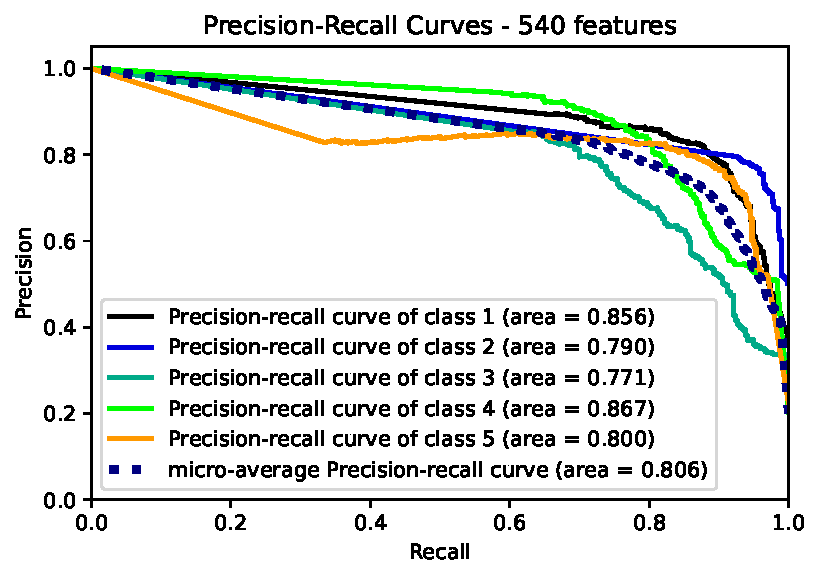
\includegraphics[width=\linewidth]{immagini Lia/precision_recall_540_w6.pdf}
    \caption{Precision-Recall Curve}
    \label{fig:prerec540}
    \end{subfigure}
    
    \caption{Result of Naive Bayes Classifier using 540 features.}\label{fig:graph540}
    
\end{figure}


In the confusion matrix of Figure \ref{fig:conmat540}, this difference can be seen, as the 334 records of class 5 are predicted correctly while 177 as SITTING activities. For the class WALKING DOWNSTAIRS, 64 records are predicted as WALKING and 75 as WALKING UPSTAIRS. 

It is quite evident that activities with the same or similar movement are often incorrectly predicted. 
Again, the precision and recall plots of each class and their respective ROC curves were plotted. The AUC of the ROC curves have values between 0.94 and 0.97, while in the precision and recall graph \ref{fig:prerec540} the area under the curve has values between 0.771 and 0.867, consistent with the measurements reported in the report.

Finally, we decided to employ the Naive Bayes algorithm also on the dataset described in Section \ref{sec:imbalancedlearning}, specifically in the point 1 of the listed strategies (in this case we did not unbalance the classes). After having identified the right set of configuration for the trained model, we inspected the results. The model predicts with an accuracy of 98\%, and correctly classifies all records of class "movement" (indicated as class 0 in the plot), and out of 1560 records of class "stationary" (class 1), it incorrectly predicts only 45 as shown in Figure \ref{fig:conmat2}.

\begin{figure}
    \centering
    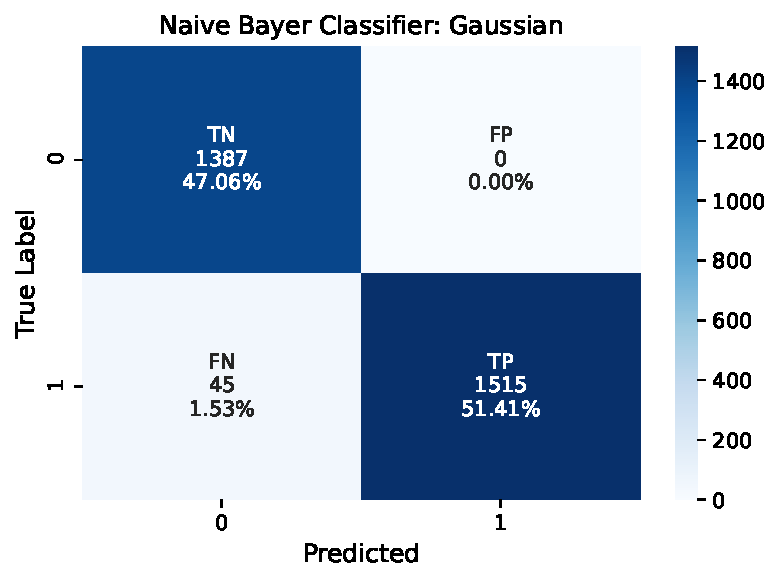
\includegraphics[width=0.5\columnwidth]{immagini Lia/confu_2_classi.pdf}
    \caption{Confusion Matrix with two classes}
    \label{fig:conmat2}
\end{figure}


After comparing the performances of all the models under analysis we concluded that the two-class models provided the highest performances. 


\subsubsection*{Logistic Regression}

The logistic regression is a classification method performed by fitting a logistic function 
%\begin{equation}
%    f(x)=\dfrac{L}{1+e^{-k_0(x-x_0)}}
%\end{equation} 
with a maximum likelihood estimation to the dataset. In a binary classification task, the output of the logistic function represents the probability that the considered record belongs to the positive class. If this value is greater than 0.5, the classifier assigns to the object the label 1, otherwise 0.

\begin{figure}
\centering
    \begin{subfigure}[t]{0.49\columnwidth}
        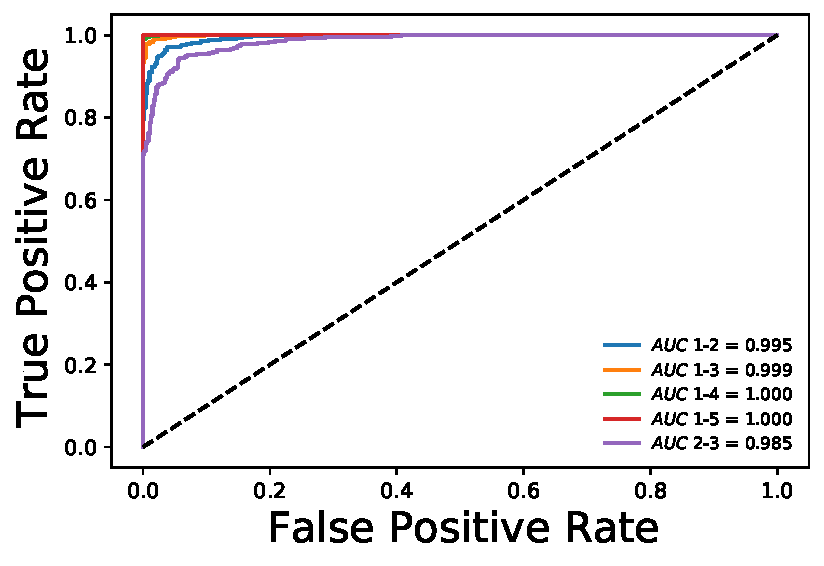
\includegraphics[width=\linewidth]{log_roc_1.pdf}
        \caption{First five pairs}
        \label{fig:logroc1}
    \end{subfigure}
  \hfill %%
    \begin{subfigure}[t]{0.49\columnwidth}
        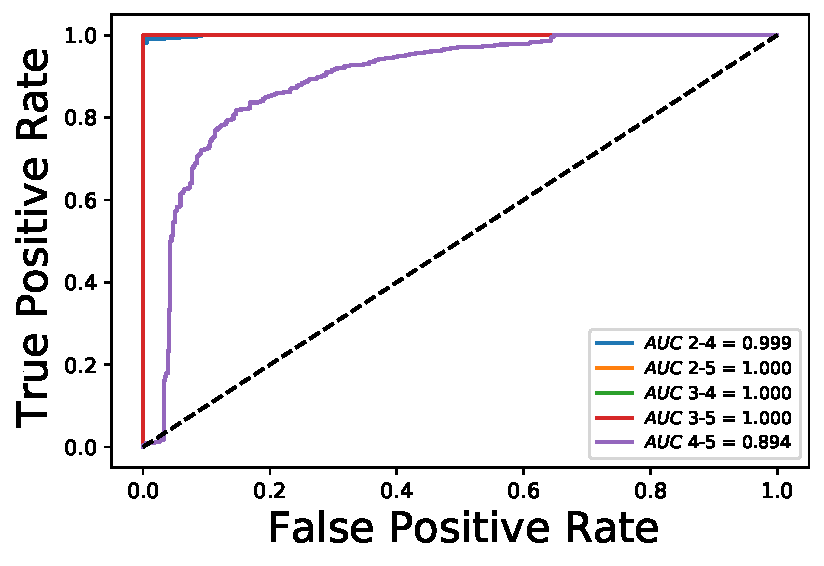
\includegraphics[width=\linewidth]{log_roc_2.pdf}
        \caption{Last five pairs}
        \label{fig:logroc2}
    \end{subfigure}
\caption{Logistic Regression: ROC and AUC of pairs}
\label{fig:logroc}
\end{figure}

To begin with, we decided to apply the logistic classifier in different binary classification scenarios. For this reason, we divided the data set in 10 subsets, containing all the possible combinations of classes. In Figure~\ref{fig:logroc} we compared all the ROC curves and AUC values obtained.

As one can see, the classifier predicts with almost perfect accuracy the majority of the pairs. The most problematic combinations were the pairs (WALKING, WALKING UPSTAIRS), (WALKING UPSTAIRS, WALKING DOWNSTAIRS), and (STANDING, LAYING). This means that these pairs of activities are very similar one from the other, so the classifier struggles more to distinguish them. 

The idea of distinguishing between pairs of classes can be extended to a classification \textit{one-versus-rest}, obtaining a multi-class classification task. One could also minimize the multinomial loss fit across the entire probability distribution, using cross-entropy. The results of this last method are shown in the classification report in Table~\ref{tab:log_multi}.

%and in the ROC curves of Figure \ref{fig:log-roc-multi}.

\begin{table}
\caption{Classification report for multiclass logistic regression.}
\label{tab:log_multi}
\centering
\resizebox{\columnwidth}{!}{
\begin{tabular}{|r|c|c|c|c|}
\toprule
{} &  precision &    recall &  f1-score &     support \\
\midrule
WALKING            &   0.85 &  0.99 &  0.92 &   496 \\
WALKING UPSTAIRS   &   0.90 &  0.83 &  0.86 &   471 \\
WALKING DOWNSTAIRS &   0.97 &  0.88 &  0.93 &   420 \\
SITTING            &   0.85 &  0.73 &  0.79 &   491 \\
STANDING           &   0.79 &  0.88 &  0.83 &   532 \\
accuracy           &   0.86 &  0.86 &  0.86 &  2410 \\
macro avg          &   0.87 &  0.86 &  0.86 &  2410 \\
weighted avg       &   0.87 &  0.86 &  0.86 &  2410 \\
\bottomrule
\end{tabular}
}
\end{table}


\begin{comment}

\begin{figure}
    \centering
    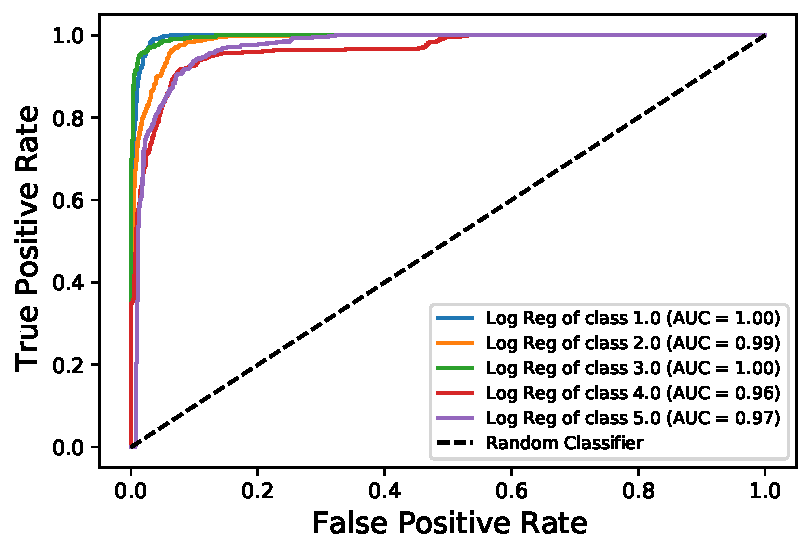
\includegraphics[width=0.8\columnwidth]{log_multiclass_roc.pdf}
    \caption{Logistic Regression: ROC and AUC for multiclass classification.}
    \label{fig:log-roc-multi}
\end{figure}

\end{comment}

\begin{figure}
    \centering
    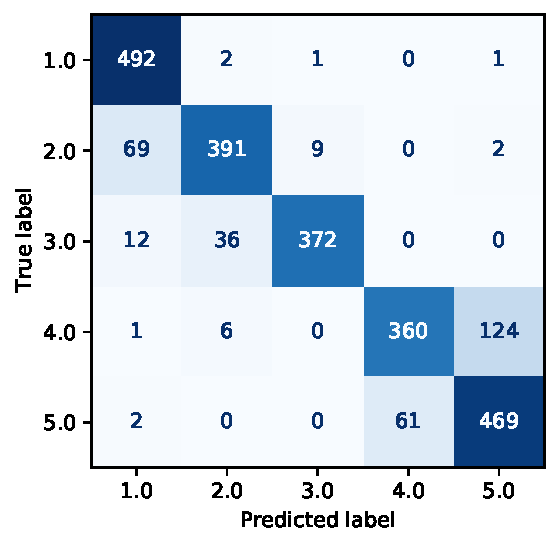
\includegraphics[width=0.4\columnwidth]{confusion_matrix_log.pdf}
    \caption{Confusion Matrix for logistic regression classification.}
    \label{fig:log_confusion}
\end{figure}

As one can see, the best classified classes, according to the F1 score, were WALKING DOWNSTAIRS and WALKING. Recalling what said for the pairwise classification task, by looking at Figure~\ref{fig:log_confusion}, it is interesting to notice how the WALKING class was not well predicted with respect to WALKING UPSTAIRS.

\subsubsection*{Support Vector Machines}

Support Vector Machines classify the records building hyperplanes in high-dimensional spaces to better separates the classes one from each other.

The tuning of the hyper-parameters was performed using a grid-search between various values of \textit{C}, \textit{gamma} and \textit{kernel}. After finding $C=10$, \textit{gamma}$=0.01$ and  \textit{kernel}=\textit{rbf}, one can see how well the classifier performs in the classification report of Table \ref{tab:svm_report}. Overall, the performances are in line with the other classifiers.

\begin{comment}
\begin{figure}
    \centering
    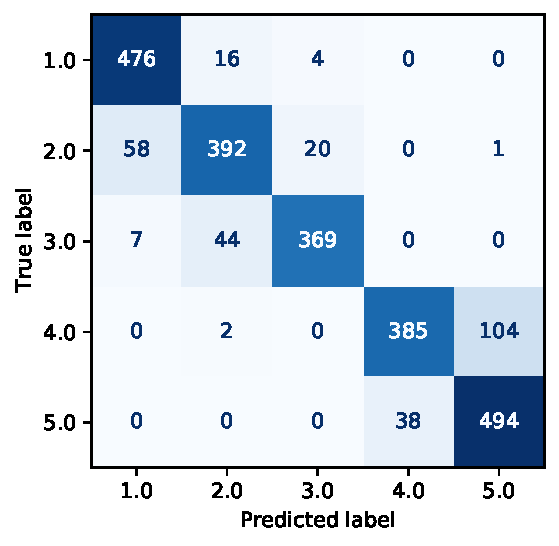
\includegraphics[width=0.6\columnwidth]{confusion_matrix_svm.pdf}
    \caption{Confusion Matrix for the SVM classifier}
    \label{fig:confusion_svm}
\end{figure}
\end{comment}

\begin{table}
\centering
\caption{Classification report for SVM}
\label{tab:svm_report}
\resizebox{\columnwidth}{!}{
\begin{tabular}{|r|c|c|c|c|}
\toprule
{} &  precision &    recall &  f1-score &     support \\
\midrule
WALKING            &   0.88 &  0.96 &  0.92 &   496 \\
WALKING UPSTAIRS   &   0.86 &  0.83 &  0.85 &   471 \\
WALKING DOWNSTAIRS &   0.94 &  0.88 &  0.91 &   420 \\
SITTING            &   0.91 &  0.78 &  0.84 &   491 \\
STANDING           &   0.82 &  0.93 &  0.87 &   532 \\
accuracy           &   0.88 &  0.88 &  0.88 &  2410 \\
macro avg          &   0.88 &  0.88 &  0.88 &  2410 \\
weighted avg       &   0.88 &  0.88 &  0.88 &  2410 \\
\bottomrule
\end{tabular}
}
\end{table}

The separation of the hyperplanes is performed in a 23-dimensional space, but, in order to visualize it, one can perform a Principal Component Analysis. The number of dimensions (three) was chosen according to the percentage of explained variance. The result is shown in Figure \ref{fig:pca_svm}, whereas the colors represent the five classes.

\begin{figure}
    \centering
    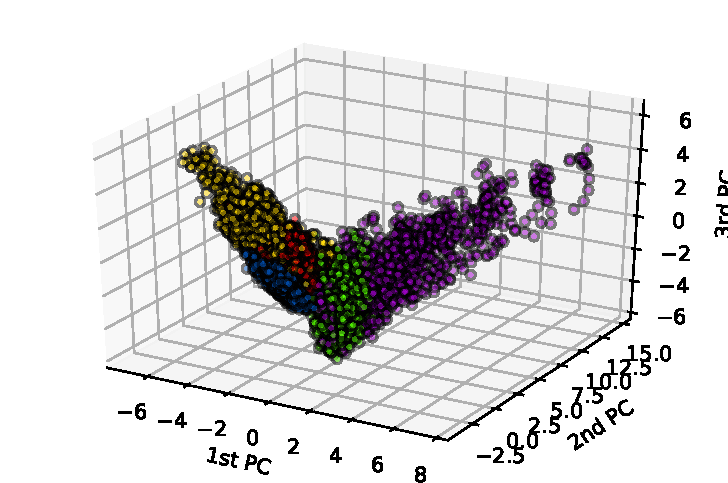
\includegraphics[width=0.8\columnwidth]{pca_svm.pdf}
    \caption{Scatter Plot in Principal Component Analysis with classified points. The color indicates the class.}
    \label{fig:pca_svm}
\end{figure}

One can also see the vectors whose Lagrange multiplier is not zero, i.e. the vectors that in a 23-dimensional space would have been at the margin of the hyperplanes separating the classes. These vector are represented in form of circles in Figure \ref{fig:vector}. 

\begin{figure}[h]
    \centering
    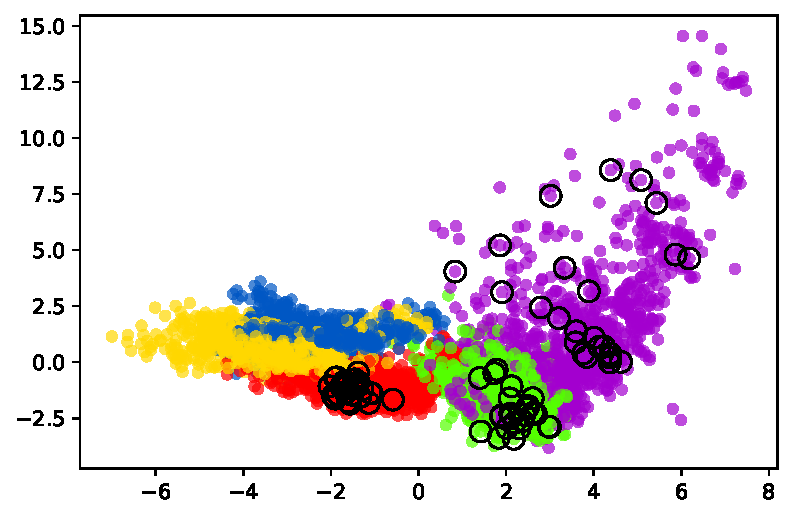
\includegraphics[width=0.6\columnwidth]{vectors.pdf}
    \caption{Vectors whose Lagrange multiplier is zero}
    \label{fig:vector}
\end{figure}

\subsubsection*{Neural Networks}

\begin{figure}
\centering
    \begin{subfigure}[t]{0.47\columnwidth}
    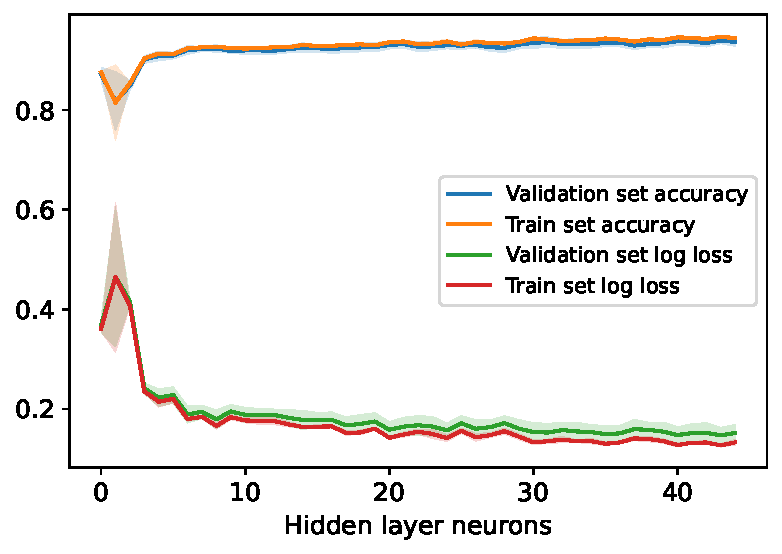
\includegraphics[width=\linewidth]{immagini simone/hidden_neurons_acc_loss.pdf}
    \caption{Variation of accuracy and cross-entropy as the number of neurons changes.}
    \label{fig:nn_hidden_neurons}
\end{subfigure}
\hfill%%
\begin{subfigure}[t]{0.49\columnwidth}
    \centering
    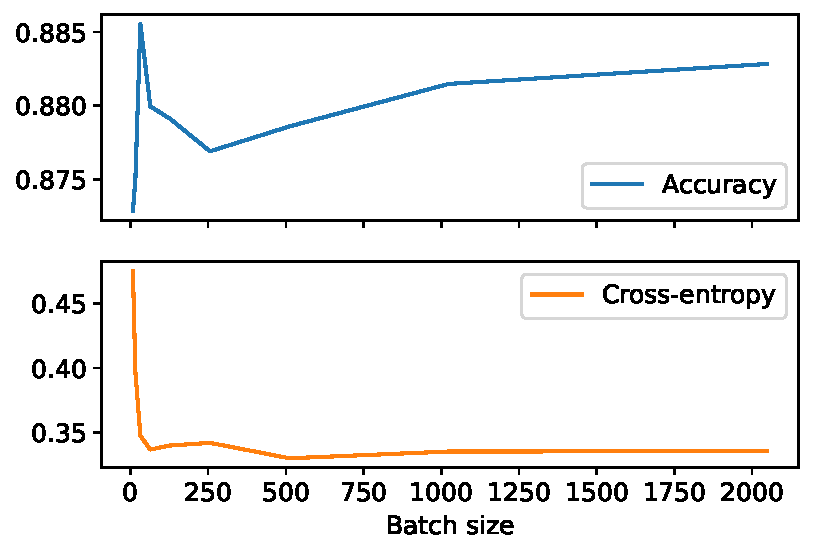
\includegraphics[width=\linewidth]{immagini simone/batch_size.pdf}
    \caption{Variation of accuracy and cross entropy as batch size increases.}
    \label{fig:nn_batch_size}
    \end{subfigure}
\caption{Neural Network: hyper-parameter tuning.}
\end{figure}

For neural networks, we used the Keras and scikit-learn libraries. We spent a lot of time trying to fine-tune the Keras network, however, unlike scikit-learn, we struggled to find the optimal configuration. Let's start by discussing the former library.

Given the high number of model parameters, we initially decided to tune one or two of them at a time. A stratified 10-fold cross-validation was used in all searches. Specifically, we began with a multilayer perceptron composed of only one hidden layer. The original idea was to tune all parameters and then try to change the number of layers. 

To find the optimal number of neurons, we first performed a grid search for each integer in the range $[2, 46]$, training each model for, at most, 100 epochs (early stopping with $\mathrm{patience}=10$). We observed high randomness in tuning this parameter. Namely, by running the algorithm several times we got different results. However, as Figure~\ref{fig:nn_hidden_neurons} shows, the higher the number of hidden neurons, the higher the accuracy score. Moreover, since train and validation sets have a very similar cross-entropy, the number of neurons does not seem to cause overfitting. The model with the highest accuracy was the one with 40 nodes.

Next, we tried to tune simultaneously the weights initializer and the activation functions. Specifically, for the activation function of the hidden layer, we tried ReLu, sigmoid, softplus, softsign, tanh, and ELU. For the weights, instead, we used all the techniques provided by Keras: truncated normal and uniform distributions, as well as zeros and ones. Moreover, we also tested the combination SELU and lacun\_normal. Despite the poor performances of fixed weights, in general, these two parameters did not seem to make a difference. In the end, the selected parameters were he\_normal initialization and tanh function.

Then, we tuned the optimizer and the learning rate. We tested Adam, SGD, RMSprop, and Nadam optimizers, while for the learning rate we searched it within the following set of values $\{0.9, 0.5, 0.2, 0.15, 0.1, 0.05, 0.01, \num{5e-3}, \num{1e-3}, \num{5e-4}, \num{1e-4},\num{5e-5}, \num{1e-5}\}$. The best model was the one with the Nadam optimizer and a learning rate equal to 0.01. 

By training a network using all these parameters together, we observed that the model was overfitting both train and validation sets. Indeed, the accuracy measured on these two sets was, approximately, 96.5\% and 97.5\%, with a cross-entropy of 0.066 and 0.078. Whereas on the test set, we got accuracy=83.15\% and loss=0.758. 

For this reason, we decided to use two different regularization techniques: dropout and $\ell_2$ penalty. In the first case, we tested the dropout rates in the following set of values $\{0.2, 0.5, 0.7\}$, while for  $\ell_2$ we used  $\{0.01, 0.05. 0.1\}$. These regularization strategies decreased the overall accuracy but did not significantly reduce the value of the loss function.

In addition, we decided to try to optimize the batch size---the number of records processed simultaneously by the network through a forward pass and then through backpropagation. This parameter improved the model's ability to generalize. We searched the batch size within the set $\{2^n|n=5,\dots,11\}$. The highest accuracy was reached with a size of 32, however, this batch is the third-last in terms of cross-entropy. On the other hand, the batch with size 2048 was the second in terms of accuracy (with a gap of only 0.3\%) and the third for what concerns the log loss (see Figure~\ref{fig:nn_batch_size}). For this reason, we decided to use this batch size. However, we noted that for a larger batch cardinality, the neural network requires more epochs to converge. Therefore, we decided to train each model for, at most, 2000 epochs and used an early stopping condition that triggered if for 20 consecutive epochs the cross-entropy value did not improve.

We also found significant improvements using a learning rate schedule. Specifically, we used the power scheduling $lr_t = lr_0 / (1 + steps / s)$, where $s=1/decay$. This parameter turned the learning rate from constant to variable. This strategy implies that after $s$ steps, the initial learning rate halved, while after $2s$ steps it becomes one-third. 

\begin{figure}
    \centering
    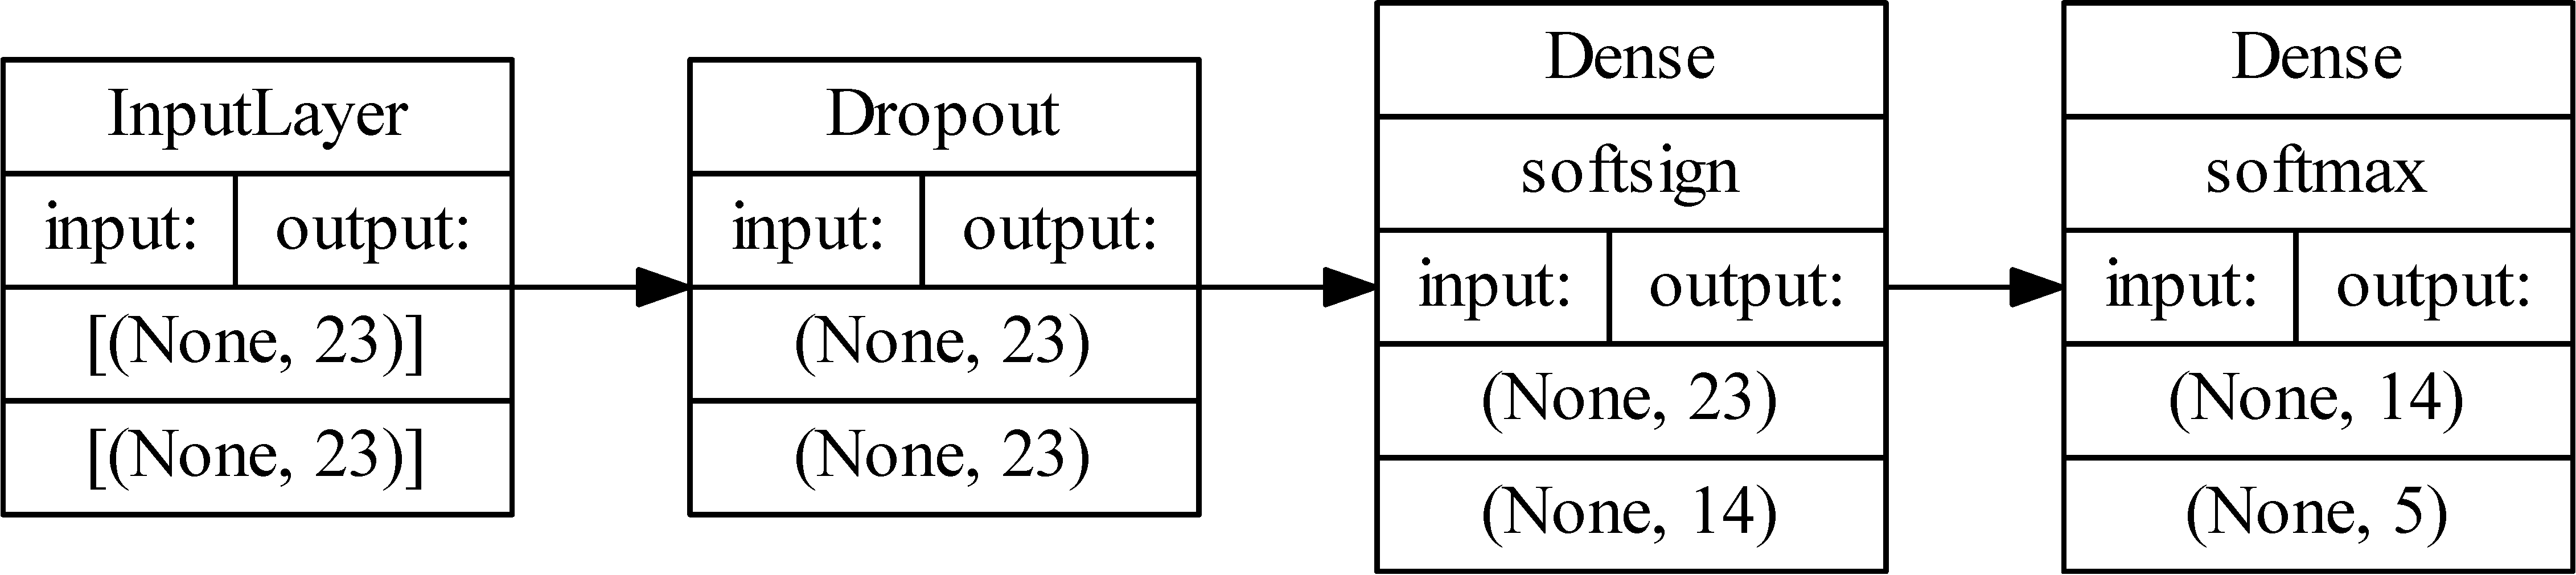
\includegraphics[width=\linewidth]{immagini simone/keras_ann_arch.pdf}
    \caption{Keras ANN Architecture.}
    \label{fig:keras_ann}
\end{figure}

Since the generalization performances were still poor, we decided to change our strategy. Instead of individually tuning the parameters, we used cross-validation scheduled in different rounds where we tuned all parameters simultaneously, zooming each time in the best region. After six rounds, we ended up with the ANN summarized in Figure~\ref{fig:keras_ann}. The architecture shows a dropout layer that randomly turns off the 5\% of the input neurons. In the middle, we have a hidden layer composed of 14 neurons. Its weights are initialized with a truncated normal distribution. Moreover, this layer uses a softsign activation function defined as $\frac{x}{|x| +1}$. For the output layer, instead, since this is a multi-class problem, we were forced to use the softmax function that computes the vector of probabilities, one for each class. The optimal network uses the Nadam otimizer (i.e., Adam with Nesterov momentum) with a 0.01 exponential decay rate (beta\_1).

Due to the random initialization of the weights, neural networks are very unstable. Therefore, to summarize the results  of the final model, we decided to train and evaluate it ten different times and then take the mean of the scores achieved. 

Compared to the results of the other classifiers used, those of the neural network we built with Keras were not exciting. On the test set we obtained the following scores: log loss value equal to 0.456 (against 0.33 of the train set), and an accuracy of 84.06\%.

\begin{figure}
    \centering
    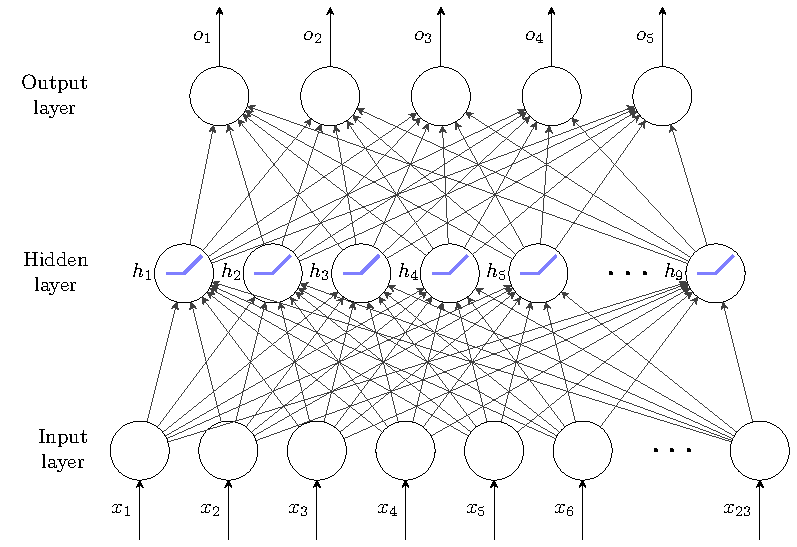
\includegraphics[width=0.7\linewidth]{immagini simone/sklearn_ann.pdf}
    \caption{Scikit-learn ANN Architecture.}
    \label{fig:sklearn_ann}
\end{figure}

On the other hand, using MLPClassifier from scikit-learn library, we found it easier to fine-tune hyperparameters. For this reason, we also achieved better performances. Again, we used a round-by-round tuning strategy. After four rounds, we ended up with the best model summarized in Figure~\ref{fig:sklearn_ann}. The hidden layer has only nine neurons and utilizes the ReLu activation function. The model uses an L-BFGS quasi-deterministic optimizer and processes the records by adopting a full-batch strategy. We trained the model for a maximum of 6000 epochs using an early stopping condition on the loss function. Moreover, the latter was penalized with an $\ell_2$ regularization parameter equal to 5. 

As we did with the Keras network, to obtain more stable estimates of the model performances we trained and evaluated the model ten different times and then computed the mean of the scores. The overall accuracy was 86.84\% while the cross-entropy 0.3417. Like the other tested classifiers, the MLPClassifier struggles with the static classes obtaining an F1 score of 79.69\% on SITTING and 83.84\% on STANDING. The confusion matrix in Figure~\ref{fig:nneval} summarizes the performances of the model, while the ROC curve depicts the higher trade-off between TPR and FPR for the static activities.

\begin{figure}[h]
    \centering
    \begin{subfigure}[t]{0.40\columnwidth}
    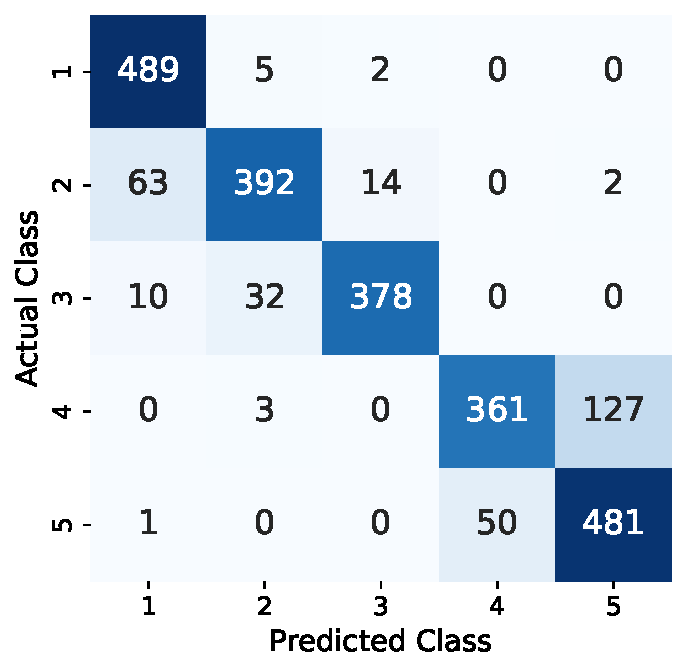
\includegraphics[width=\linewidth]{immagini simone/conf_mtx_sklearn_ann.pdf}
    \caption{Confusion Matrix}
    \label{fig:nnconf}
\end{subfigure}
\hfill%%
\begin{subfigure}[t]{0.55\columnwidth}
    \centering
    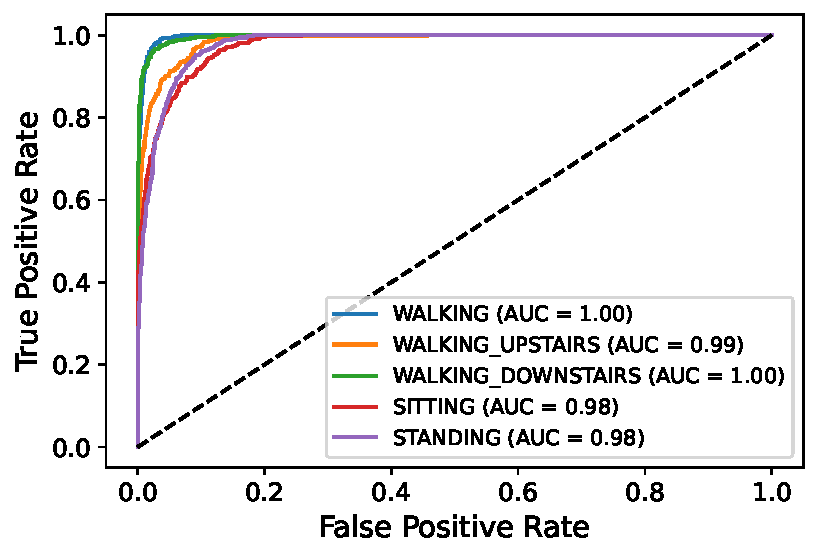
\includegraphics[width=\linewidth]{immagini simone/roc_sklearn_ann.pdf}
    \caption{ROC Curve.}
    \label{fig:nnroc}
    \end{subfigure}
\caption{Scikit-learn Neural Network: evaluation curves.}
\label{fig:nneval}
\end{figure}


\subsubsection*{Ensemble Methods}

Ensemble methods build and combine the predictions of many estimators. They improve the performances of the base classifiers used in the ensemble by reducing their variance or bias. Generally speaking, there exist two principal families of ensemble methods:
%
\begin{itemize}
    \item Averaging methods that build independent estimators and then average their predictions using, for instance, a majority vote. They aggregate unstable base classifiers attempting to reduce their variance. Regarding this family, we will discuss the random forest meta-estimator.
    \item Boosting methods that build sequential base estimators, each of which improves the predictions made by the previous estimators. They aggregate stable base classifiers attempting to reduce their bias. Concerning this family, we will deal with AdaBoost and gradient boosting.
\end{itemize}

\begin{table}[h]
\centering
\caption{Classification report for Random Forest}
\label{tab:rf_report}    
\resizebox{\columnwidth}{!}{
\begin{tabular}{|r|c|c|c|c|}
\toprule
{} &  precision &    recall &  f1-score &     support \\
\midrule
WALKING            &   0.87 &  0.97 &  0.92 &   496 \\
WALKING UPSTAIRS   &   0.86 &  0.87 &  0.86 &   471 \\
WALKING DOWNSTAIRS &   0.97 &  0.84 &  0.90 &   420 \\
SITTING            &   0.86 &  0.76 &  0.80 &   491 \\
STANDING           &   0.80 &  0.89 &  0.84 &   532 \\
accuracy           &   0.87 &  0.87 &  0.87 &  2410 \\
macro avg          &   0.87 &  0.86 &  0.87 &  2410 \\
weighted avg       &   0.87 &  0.87 &  0.86 &  2410 \\
\bottomrule
\end{tabular}
}
\end{table}

\paragraph{Random Forest}
is a bagging method that consists in creating different bootstrapped datasets from the training sets and developing for each one a decision tree (more generally, an \textit{estimator}). Then, each record is evaluated by every tree (a.k.a. by the \textit{forest}) and classified according to the majority of the outputs.

The tuning of the hyper-parameters was performed using a cross-validation with 5 folds. The results are shown in the classification report in Table~\ref{tab:rf_report}.

\begin{comment}
\begin{figure}
    \centering
    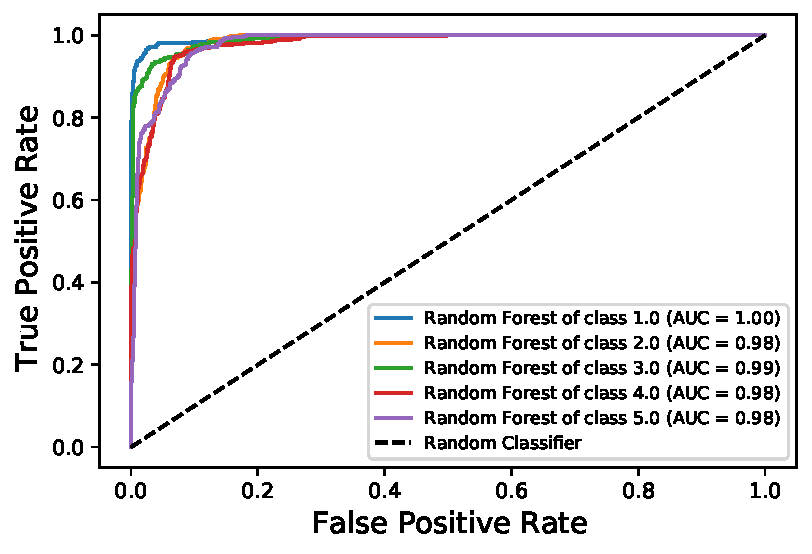
\includegraphics[width=0.8\columnwidth]{RF_multiclass_roc.pdf}
    \caption{Random Forest: ROC and AUC}
    \label{fig:rf-roc}
\end{figure}
\end{comment}

In Figure \ref{fig:accuracy_rf} is shown how the number of estimators influences the accuracy of the model. As illustrated, the accuracy fluctuates between 0.861 and 0.865, thus producing good performances for each configuration.

\begin{figure}

    \centering
    \begin{subfigure}[t]{0.49\columnwidth}
    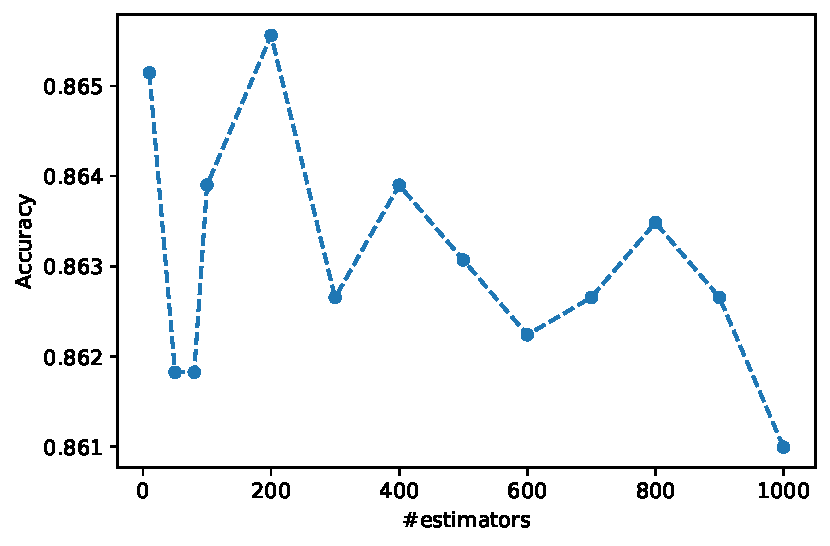
\includegraphics[width=\linewidth]{RF_accuracy.pdf}
    \caption{Accuracy vs number of estimators}
    \label{fig:accuracy_rf}
\end{subfigure}
  \hfill %%
\begin{subfigure}[t]{0.49\columnwidth}
    \centering
    \includegraphics[width=\linewidth]{RF_maxsamples.pdf}
    \caption{Accuracy vs max number of samples (in percentage)}
    \label{fig:maxsamples_rf}
    \end{subfigure}
    \caption{Variation of Accuracy in Random Forest}
    
\end{figure}

Another way to determine the number of estimators consists in running different simulations and picking the value with the lowest \textit{Out Of Bag error}, i.e. the misclassification error on the records that did not enter the bootstrapped dataset.
This measure does not show interesting results, so it was chosen not to discuss it in the report.

In an ensemble classifier, a degree of freedom is given by the max number of samples to draw to construct the bootstrap dataset.
In Figure \ref{fig:maxsamples_rf} one can see how the value of the accuracy is very low for every value less than 0.001 and grow significantly to remain stable. One can conclude that the minimum percentage needed to build each bootstrapped dataset is 1\% of the total frame.

Random Forest are also a useful tool to study the feature importance using the gini or mean decrease impurity method. In fact, in a decision tree, one can see how each feature decrease the impurity of the split (the feature with highest decrease is selected for internal node). So for each feature one can collect how on average it decreases the impurity and the average over all trees in the forest is the measure of the feature importance. 

The results of this analysis are shown in form of a bar chart in Figure~\ref{fig:importance_rffi}. 

One can compare the results with another method of feature importance study, e.g. the permutation importance, reported in Figure \ref{fig:permutation_importance}. Both the analysis reveal that the most important feature is the magnitude of the body acceleration energy in the frequency domain. Other features are shared, although there are some dissimilarities.

\begin{figure}
    \centering
    \begin{subfigure}[t]{0.49\columnwidth}
    \includegraphics[width=\linewidth]{RF_importance.pdf}
    \caption{First seven Random Forest Feature Importance (Gini)}
    \label{fig:importance_rffi}
\end{subfigure}
  \hfill %%
\begin{subfigure}[t]{0.49\columnwidth}
    \includegraphics[width=\linewidth]{random_importance.pdf}
    \caption{First seven Permutation Importance}
    \label{fig:permutation_importance}
    \end{subfigure}
    \caption{Feature Importance: a comparison}\label{fig:rf_importance}
\end{figure}

\paragraph{AdaBoost} is an ensemble method based on boosting, instead of bagging. The main difference between these two kind of approaches is that boosting adaptively change distribution of training data by focusing more on previously misclassified records. Boosting assign weights to the records to classify that may change during the boosting procedure.

A grid search is performed to tune the hyperparameters, i.e. the number of estimators and the learning rate. The results of the classification are reported in Table \ref{tab:ab_report}.

\begin{table}
\centering
\caption{Classification report for Ada Boost}
\label{tab:ab_report}
\resizebox{\columnwidth}{!}{
\begin{tabular}{|r|c|c|c|c|}
\toprule
{} &  precision &    recall &  f1-score &      support \\
\midrule
WALKING            &   0.72 &  0.97 &  0.83 &   496 \\
WALKING UPSTAIRS   &   0.82 &  0.75 &  0.78 &   471 \\
WALKING DOWNSTAIRS &   0.95 &  0.65 &  0.77 &   420 \\
SITTING            &   0.78 &  0.45 &  0.57 &   491 \\
STANDING           &   0.63 &  0.88 &  0.74 &   532 \\
accuracy           &   0.75 &  0.75 &  0.75 &  2410 \\
macro avg          &   0.78 &  0.74 &  0.74 &  2410 \\
weighted avg       &   0.77 &  0.75 &  0.74 &  2410 \\
\bottomrule
\end{tabular}
}
\end{table}

In Figure \ref{fig:ada_accuracy} is shown how the number of estimators influences the accuracy of the model. The best performing model has 30 estimators. For high number of estimators the accuracy stabilize at 0.68.

In opposition to random forest, AdaBoost is not influenced by the max samples, as one can see in Figure \ref{fig:ada_max}

\begin{figure}
    \centering
    \begin{subfigure}[t]{0.49\columnwidth}
    \includegraphics[width=\linewidth]{Ada_accuracy.pdf}
    \caption{Accuracy vs number of estimators}
    \label{fig:ada_accuracy}
\end{subfigure}
  \hfill %%
\begin{subfigure}[t]{0.49\columnwidth}
    \includegraphics[width=\linewidth]{Ada_maxsamples.pdf}
    \caption{Accuracy vs maximum number of samples (in percentage)}
    \label{fig:ada_max}
\end{subfigure}
\caption{Variation of Accuracy in AdaBoost}\label{fig:ada_acc}
\end{figure}

\subsubsection*{Gradient Boosting Machines}

Gradient boosting is a general technique that uses many sequentially built weak learners---typically,  shallow decision trees---to predict the residuals of the previous estimators in the ensemble. In doing so, it tries to optimize a loss function using the gradient descent technique. We tested three algorithms that implement this strategy: GradientBoostingClassifier (scikit-learn); XGBoost (The XGBoost Contributors); LightGBM (Microsoft).

\paragraph{GradientBoostingClassifier} The model applied without modifying the default parameters obtained excellent performances. The accuracy was equal to 87.93\%, and the F1 scores on dynamic classes were around 88\%-93\%.

Due to the slowness of the algorithm, we decided to tune the hyperparameters in 5 rounds, zooming into the best region each time using a stratified 5-folds cross-validation. We evaluated the best parameters with respect to accuracy and log loss measures. We noticed that the latter was able to identify parameters capable of better generalization, so we used the log loss as our main driver.

At first, for the specified parameters, we used the following wide range of values: learning rate $\{0.01, 0.1, 0.5\}$, number of estimators $\{50, 250, 500\}$, subsample $\{0.25, 1\}$, and max depth $\{2, 5\}$. Note that for multi-class problems, the n\_estimators parameter does not indicate the number of base classifiers in the ensemble, but the number of boosting iteration. Indeed, for these class of problems, at each iteration, the gradient boosting methods build an estimator for each class. Therefore, since we are dealing with 5 classes, the number of potential estimators in the ensemble goes from 250 to 2500. 

After the last-tuning round, the best model was trained using a learning rate equal to 0.25 for 55 boosting iteration, thus producing an ensemble of 275 decision trees having depth 4. Moreover, the best value for the subsample parameter was 0.67, meaning that, at each iteration, the estimators were trained using a 67\% random sample drawn without replacement from the original data.

The best model just outlined obtained an overall accuracy of 88.09\%, performing well on both static and dynamic classes. The confusion matrix in figure~\ref{fig:gbclassifier} is very similar to those already discussed and suggests that the two macro-classes are well separated.  

\begin{figure}
    \centering
    \begin{subfigure}[t]{0.40\columnwidth}
    \includegraphics[width=\linewidth]{immagini simone/gbclassifier_conf_mtx.pdf}
    \caption{Confusion Matrix.}
    \label{fig:gbclassifier_confusion}
\end{subfigure}
  \hfill %%
\begin{subfigure}[t]{0.55\columnwidth}
    \includegraphics[width=\linewidth]{immagini simone/gbclassifier_roc.pdf}
    \caption{ROC curve.}
    \label{fig:gbclassifier_roc}
\end{subfigure}
\caption{GradientBoostingClassifier Evaluation}
\label{fig:gbclassifier}
\end{figure}

\paragraph{XGBoost} XGBoost is an optimized version of the scikit-learn GradientBoostingClassifier. Indeed, thanks to its aggressive regularization and pruning policies, it manages to be dozens of times faster. Furthermore, it generarly produces better risults. In our case, the model with the defaults prameters reached an accuracy of 88.88%. 

XGBoost does not use plain regression trees like the GradientBoostingClassifier. One of the main differences is that rather than computing the gain of each split in terms of MSE, it uses the similarity score. Moreover, it introduces the gamma parameter that, together with the regularization terms, operates as an aggressive pruning strategy. 

As we did for the GradientBoostingClassifier, we tuned the XGBoost parameters using different cross-validation rounds, selecting the best parameters with respect to a combination of accuracy and log loss scores. First we tried to figure out the correct number of boosting iteration and the magnitude of the learning rate. We noted that there exists a trade-off between these two parameters. Overall, we performed eight tuning rounds, zooming in the best region of all the main parameters. In the end, the best model we found, has the following architecture: number of estimators $=375$, learning rate $=0.3$, max depth $=2$, subsample $=0.25$, gamma $=0.25$, reg lambda $=15$, and reg alpha $=5$. Interestingly, at each boosting iteration, it only used 25\% of the samples to train the estimators. 

The optimal model achieved an overall accuracy of 89.59\% and, as can be seen from the confusion matrix in Figure~\ref{fig:xgboost}, behaves very similarly to the vanilla model. Moreover, compared with all other models tested in this project, the ROC curve shows very little trade-off between TPR and FPR. The reason for this is that XGBoost was also able to perform excellently with the SITTING and STANDING classes, achieving F1 scores of 87\% and 89\%, respectively.

\begin{figure}
    \centering
    \begin{subfigure}[t]{0.40\columnwidth}
    \includegraphics[width=\linewidth]{immagini simone/xgboost_conf_mtx.pdf}
    \caption{Confusion Matrix.}
    \label{fig:xconfusion}
\end{subfigure}
  \hfill %%
\begin{subfigure}[t]{0.55\columnwidth}
    \includegraphics[width=\linewidth]{immagini simone/xgboost_roc.pdf}
    \caption{ROC curve.}
    \label{fig:xroc}
\end{subfigure}
\caption{XGBoost Evaluation.}
\label{fig:xgboost}
\end{figure}

\paragraph{LightGBM} is the fastest gradient boosting implementation discussed in this project. It is efficient in terms of both training time and memory usage. It also performs very well with default parameters, achieving, in our case, an accuracy of 89.21\% .

The main idea of this algorithm is to order and discretize each continuous feature of the dataset using histogram bins. In addition, the estimators within the ensemble are not built level by level, but by exploring each time the leaf that is supposed to produce the largest decrease in loss.

Like for the other two discussed gradient boosting techniques, we tuned the model hyperparameters using a multiple rounds strategy. 

The parameters of LightGBM are pretty much the same as those already discussed for the previous two models, so we initially specified very similar search ranges. In addition, we tried adjusting the maximum number of bins per feature and the minimum cardinality of each bin. However, the best performance was achieved with the default values, namely: max bin $=255$ and min data in bin $=3$. 

After seven tuning rounds, the best model was the one with the following parameters: max bin $=255$, learning rate $=0.25$, number of estimators $=100$, max depth $=2$, min data in bin $=3$, min split gain $=0.05$, reg  alpha $=1$, reg lambda $=15$, bagging fraction $=0.25$, bagging freq $=1$.

With an accuracy of 89.75\%, this was the best classifier used so far. However, the XGBoost algorithm performed slightly better for static classes.

In conclusion, as we did for the other models. Figure~\ref{fig:lightgbm} shows the confusion matrix and ROC curve of the LightGBoost classifier.

\begin{figure}
    \centering
    \begin{subfigure}[t]{0.40\columnwidth}
    \includegraphics[width=\linewidth]{immagini simone/lightgbm_conf_mtx.pdf}
    \caption{Confusion Matrix.}
    \label{fig:lcla}
\end{subfigure}
  \hfill %%
\begin{subfigure}[t]{0.55\columnwidth}
    \includegraphics[width=\linewidth]{immagini simone/lightgbm_roc.pdf}
    \caption{ROC curve.}
    \label{fig:lroc}
\end{subfigure}
\caption{LightGBM Evaluation}
\label{fig:lightgbm}
\end{figure}

\subsection{Regression}

\subsubsection*{Simple Linear Regression}

We decided to use linear regression to predict the continuous values of the chosen dependent variable (see later). The analysis was carried out on the training set consisting of 23 features. Since the dataset contains activities belonging to two different macro-classes (activities that require efforts such as WALKING and passive activities such as LAYING), we filtered the records by separating those belonging to the "stationary" macro-class from those belonging to the "dynamic" macro-class.

We considered it appropriate to show only the most interesting results even though the analysis was carried out on several combinations of feature pairs. For the selection of the variables, we examined the correlation and used for the analysis only those having the highest correlation. We then fixed the dependent variable “tGravityAcc-mean()-X” and we inspected the performance of the regressor as we changed the independent variable. We also examined the difference in the prediction when we used as independent variables those having a low correlation with the dependent one. By doing so we noticed that under these conditions the error increases as the data are not linearly distributed, hence they cannot be approximated by a simple linear regressor.

The selected dependent variable is highly correlated with the variables "tGravityAcc-min()-X" and "angle(Y,gravityMean)”---96\% and 64\%, respectively---, for this reason, we decided to show the linear regression results using these two attributes.

As we expected, the best fit was obtained with the 'tGravityAcc-min()-X" independent variable (see Figure~\ref{fig:linear}). Analyzing the $R^2$ score, we can notice that the variable “tGravityAcc-min()-X” is able to predict almost 96\% of the variance of the dependent variable. On the test set, the model has an MSE of 0.00 and an MAE is 0.007. As it can be seen, the results are close to perfection as the error is near the lowest possible value.

\begin{figure}
    \centering
    \begin{subfigure}[t]{0.48\columnwidth}
    \includegraphics[width=\linewidth]{immagini Lia/linear regression lineare.pdf}
    \caption{tGravityAcc-min()-X as independent variable.}
    \label{fig:linear}
\end{subfigure}
\hfill
\begin{subfigure}[t]{0.49\columnwidth}
    \includegraphics[width=\linewidth]{immagini Lia/linear regression parabolica.pdf}
    \caption{angle(Y,gravityMean) as independent variable.}
    \label{fig:parabolic}
\end{subfigure}
\caption{Linear regression with the tGravityAcc-mean()-X dependent variable, changing the independent variable.}
\label{fig:linearregression}
\end{figure}

On the contrary, by changing the independent variable to "angle(Y,gravityMean)”, the data distribution becomes parabolic (see Figure~\ref{fig:parabolic}). Examining it visually we quickly noticed that a simple straight line could not catch the way data are distributed into the 2-dimensional space, hence we expected a lower $R^2$ score. Indeed, on the training set, we observed an $R^2$ of 0.415, while on the test, its score is negative (-0.644).  One reason for this can be attributed to the fact that the prediction problem is not linear hence it cannot be approximated by linear regression.  This can also be seen  by looking at Figure~\ref{fig:actual}, where we can compare the frequency with which actual and predicted values appear for the "angle(Y,gravityMean)” attribute. 
In conclusion, using the “angle(Y,gravityMean)” for predicting "tGravityAcc-mean()-X" is not an optimal choice, because the model is not able to generalize well.

\begin{figure}
    \centering
    \includegraphics[width=0.6\columnwidth]{immagini Lia/actual vs predicted.pdf}
    \caption{Actual vs predicted values in the simple linear regression for the “angle(Y,gravityMean)” independent variable. Values between 0.65 and 1.2 are predicted fewer times than they appear in the distribution.}
    \label{fig:actual}
\end{figure}

\begin{figure}[h]
    \centering
    \includegraphics[width=\columnwidth]{r2_lin.pdf}
    \caption{$R^2$ value for each multilinear regression performed. The name of the variable on the y-axis indicates which variable is considered dependent from all the others.}
    \label{fig:r2_lin}
\end{figure}

\subsubsection*{Multiple Linear Regression}

Since there is not a linear regression task in the dataset, it was decided to perform also a multilinear regression on each one of the 23 selected features using the other 22 variables as the function support. 

To validate how well the models perform, the $R^2$ value of each linear fit is plotted in the bar chart of Figure \ref{fig:r2_lin}. One can see that the best performing ones are the ones built for the features tGravityAcc-mean()-X, tGravityAcc-min()-X and angle(Y,gravityMean), while tGravityAcc-max()-Z is the worst one. The variable fBodyGyro-maxInds-X has an $R^2$ of 0.

This kind of analysis is useful also to create a "multi-correlation" heatmap. In fact, the pearson or spearman correlations are defined only for a tuple of variables. In this analysis one can see how a feature is correlated to all the other variables at the same time. To a better understanding, everything is scaled with the L2 norm. This result is shown in Figure \ref{fig:lin_heatmap}.

\begin{figure}
    \centering
    \includegraphics[width=0.60\columnwidth]{lin_heatmap.pdf}
    \caption{Heatmap with the coefficients of the linear regression for the 23 selected features}
    \label{fig:lin_heatmap}
\end{figure}

\paragraph{Lasso} is a type of linear regression in which the sums of squared residuals is penalized by the l1 score (absolute value). This method is particularly efficient when there are spurious degree of freedom for the model, letting some coefficient go to zero. In our case, letting the hyperparameter alpha to 1, all coefficients for every fits were zero, so a tuning of the alpha is needed. 

It was chosen to analyze only some features instead of all 23 like in the previous paragraph. The chosen ones are the features tGravityAcc-mean()-X, tBodyAcc-correlation()-X,Y, fBodyGyro-maxInds-X given their values of $R^2$. 

The tuning was performed running the codes with different values of alpha and picking the one returning the highest $R^2$ score.
The results of this search is plotted in Figure \ref{fig:tuning_lasso}.

As one can see, there is a significant improved for the score of the feature tGravityAcc-mean()-X, while the others do not have such growth. The best value of alpha is the same for the three features and is fixed at 0.001.

\begin{table*}[t]
    \caption{Coefficients of the Linear Regression with the Lasso/Ridge Penalty: a comparison.}
    \label{tab:lassoridge2}
    \adjustbox{max width=\textwidth}{%
    \centering
    \begin{tabular}{|c||c||c|c|c|c|c|c|c|c|c|c|c|}
    \hline
    Feature & Penalty & c1  & c2 & c3 & c4 & c5 & c6 & c7& c8 & c9 & c10 & c11\\\hline\hline
    \multirow{2}[2]*{Gravity} & Lasso & 0 & 0 & 0 & 1.01 & 0 & 0 & 0 & 0 & -0.01 & 0.01 & 0\\
    & Ridge & -1.23e-03 &  5.62e-02 &  1.71e-01 &  1.01e+00 &
  -6.23e-02 & -1.71e-01 & -3.58e-03 & -1.69e-02 &
  -3.07e-03 & -8.88e-04 &  2.37e-03 \\\hline
  
    \multirow{2}[2]*{tBody} & Lasso & -0.18 & -0.03 & 0 & -0.16 & -0.01 & -0.10 & -0.26 & 0 & 0.05 & 0 & -0.06 \\
    & Ridge & -0.24 & -0.48 & 0.40 & -0.17 & -0.21 & -0.52 &
  -0.40 & -0.01 & 0.08 & 0.13 & -0.23 \\\hline
  
  \multirow{2}[2]*{fBody} & Lasso & -0.03 & 0 & 0 & 0 & 0 & 0 & 0 & 0 & 0.02 & 0.07 & -0.02 \\
  & Ridge & -0.032 & -0.01 &  0.24 &  0.05 &  0.04 & 0.04 &
  -0.04 & 0.08 & 0.06 & 0.07 & -0.20 \\\hline
    \end{tabular}
    }
    %\caption{First eleven coefficients of the Linear Regression with the Lasso/Ridge Penalty: a comparison}
    % \label{tab:lassoridge1}
\end{table*}

\begin{table*}[t]
    \centering
    \adjustbox{max width=\textwidth}{%
    
    \begin{tabular}{|c||c||c|c|c|c|c|c|c|c|c|c|c|}
    \hline
    Feature & Penalty & c12  & c13 & c14 & c15 & c16 & c17 & c18& c19 & c20 & c21 & c22\\\hline\hline
    \multirow{2}[2]*{Gravity} & Lasso & 0.01 & 0 & 0.01 & -0.08 & -0.06 & 0 & -0.06 & 0.03 & -0.29 & -0.18 & 0\\
    & Ridge & -6.02e-03 & 2.83e-03 & -1.05e-03 &  7.11e-04 & -7.52e-03 & 6.17e-03 & -1.20e-04 & -2.21e-03 & 2.16e-02 &
  -9.85e-03 & -1.13e-02 \\\hline
  
    \multirow{2}[2]*{tBody} & Lasso & 0.01 & 0 & 0.01 & 0.08 & -0.06 &  0 & 0.06 & 0.03 & -0.29 & -0.19 &  0 \\
    & Ridge & 0.05 & 0.01 &  0.02 & -0.14 & -0.09 & 0.21 & -0.08 & 0.05 & -0.39 & -0.27 & -0.88 \\\hline
  
  \multirow{2}[2]*{fBody} & Lasso & 0 & 0& 0.05 & -0.01 & 0.06 & 0 & 0 & 0.09 & 0 & 0 & 0 \\
  & Ridge & 0.18 & -0.07 & 0.15 &  -0.02 & 0.07 & -0.03 & 0.13 &
   0.10 & 0.20 & -0.21 & 0.40\\\hline
    \end{tabular}
    }
\end{table*}

\paragraph{Ridge} is a type of linear regression in which the sums of squared residuals is penalized by the l2 score (square). As opposition of the Lasso Regression, the coefficients can go arbitrarily small, but not to zero.

By default, the alpha hyperparameter is set to 1. As with the Lasso regression, we tried tuning this parameter, but the best performance was obtained with $alpha=1$. The Ridge regressor produced results similar to those obtained with the multilinear regression. Therefore, since there are no significant improvements, we decided not to report them.

One could however compare the coefficients found with the Lasso Regression to see if the described asymptotic behaviour is observed. These results are reported in Table \ref{tab:lassoridge2}. 


One can see that in the Lasso Regression the coefficients go to zero, in opposition to the Ridge one, where they are small, but not zero. This result is in line with what one could expect from theory.

\begin{figure}[h]
    \centering
    \includegraphics[width=0.6\columnwidth]{alpha_tuning.pdf}
    \caption{Tuning of alpha for different features using Lasso Regression}
    \label{fig:tuning_lasso}
\end{figure}

\subsubsection*{Gradient Boosting Regression}

For the gradient boosting regression task, we decided to use only the scikit-learn GradientBoostingRegressor algorithm. For the \textit{univariate regression} scenario, we chose two moderately linearly correlated variables (44\%) that do not seem to measure the same phenomena, that is, tGravityAcc-arCoeff()-Y,3 and tBodyAccMagarCoeff()1.

To began with, we ran the regression without changing any parameters. Testing the model on both the train and test set, we obtained approximately the same mean squared errors: 0.059 and 0.057, respectively. As expected, the model performed worse on the test set. Indeed the gap between the coefficients of determination $R^2$ computed on the two sets of data was roughly 0.08. Generally speaking, the goodness of fit was low on both train and test set (0.25 vs 0.17).

We tried to tune the model hyperparameters following the same strategy already discussed for the classification task. Before that, we analyzed the model behavior when changing the number of estimators in the ensemble or the learning rate, leaving all other parameters at their default values. Figure~\ref{fig:gbregressor}, interestingly, suggests that the model overfits the train set even from very low levels of complexity. 

\begin{figure}[b]
\centering
    \begin{subfigure}[t]{0.32\columnwidth}
        \includegraphics[width=\linewidth]{immagini simone/gbreg_estimators_mse.pdf}
        \caption{MSE vs number of estimators}
        \label{fig:mse_gb}
    \end{subfigure}
    \hfill%
    \begin{subfigure}[t]{0.32\columnwidth}
        \includegraphics[width=\linewidth]{immagini simone/gbreg_estimators_r2.pdf}
        \caption{$R^2$ vs number of estimators}
        \label{fig:R2_gb}
    \end{subfigure}
    \hfill%
    \begin{subfigure}[t]{0.32\columnwidth}
        \includegraphics[width=\linewidth]{immagini simone/gbreg_lr_r2.pdf}
        \caption{$R^2$ vs learning rate}
        \label{fig:R2_ga}
    \end{subfigure}
\caption{GradientBoostingRegressor: overfitting analysis}
\label{fig:gbregressor}
\end{figure}

We performed four different cross-validations, zooming each time in the region of the parameters space that produced higher $R^2$ and smaller MSE. The best model that emerged from this analysis had the following parameters: 70 stumps, learning rate equal to 0.095, 25\% of sub-sample, and a minimum decrease in impurity to perform a split equal to 0.1. However, in the end, we got almost exactly the same performances of the of the default model. 

On the other hand, for the \textit{multivariate regression} scenario, we chose to work with the same target variable used for the univariate task.

First, we used all 22 variables in the dataset to run the GradientBoostingRegressor algorithm without changing the default parameters. Since the coefficient of determination always increases when using more independent variables, we decided to use the adjusted value $\hat{R}^2$ together with the MSE to evaluate the performance of the models. With the feature importances returned by the model, we performed a sort of feature selection. Specifically, we trained and evaluated (on the validation set) 22 models. We started with the best 22 features, and at each iteration we removed the least important one. The model with the best 15 features in terms of importances reached the highest $\hat{R}^2$ and the smallest MSE, respectively, 0.733 and 0.021. For this reason we decided to tune the GBRegressor using these 15 features.

We used the same strategy already discussed. We tuned the model in four different rounds zooming each time in the best region. 

The final model was much more complex than that found for the univariate task. Namely, it uses an ensemble of 150 regression trees with depth 5. Each of them was trained on an 80\% random sample of the all train set and using pruning condition based on the minimum decrease in impurity equal to 1\%.

Once again, we did not get significant improvements. The tuned model behaves very similarly to the model with 22 features using the default parameters. Specifically, we obtained about a 2\% increase in $\hat{R}^2$ and a 0.02\% decrease in MSE.

\section{Time Series Analysis}

\subsection{Introduction} \label{sec:time_series_introduction}

As already discussed in the introduction, the researchers of the original study collected the data through sensors embedded in a smartphone. Namely, data were derived from three signals: total acceleration, body acceleration, and angular velocity. For each type of signal, we have the 3-axial readings. Raw data are allocated in nine different datasets, stored in the Inertial Signals folder, each of them having 7352 objects. The sensor signals were sampled in fixed-width sliding windows of 2.56 seconds and 50\% overlap. Then, each row of the datasets represents a window composed of 128 readings. For this reason, each row can also be intended as a time series with 128 timestamps, one every 0.02 seconds. 

To deal with the time series tasks, for each activity, we reconstructed the signal of each participant. Before doing this, since now we are using raw signals, we decided to remove the effect of the sliding windows. Indeed, the original authors used this technique as a pre-processing step to build the engineered features. Our purpose is to clean the signals from redundant information. Moreover, this produces shorter time series and speeds up the computational time of our algorithms.  Therefore, we only maintained the first 64 readings for each row, discarding the remaining. However, since the last 64 readings of the last row in the dataset are not repeated, we create a new row containing these data. After this, our nine datasets has shape $7353 \times 64$. Eventually, we grouped by each subject and each activity and concatenate all the readings. Furthermore, to be consistent with the first part of the project, we decided to remove the LAYING activity.

\begin{figure}[b]
	\centering
	\includegraphics[width=\columnwidth]{immagini simone/output_46_0.pdf}
	\caption{Accuracy produced by the KNN classifier on single datasets using the Euclidean distance. Both 128 and 64 timestamps versions are evaluated.}
	\label{fig:file_accuracy}
\end{figure}
 
Since there are 21 subjects in the train sets and 9 in the test sets, we ended up with nine train datasets, each composed of $21 \cdot 5=105$ rows (time series). Since the gravitational force is assumed to be constant, initially we also decided to not take into consideration the three datasets related to the total acceleration. We concatenated the remaining 6 datasets together to form a unique dataset composed of 105 time series and 6 dimensions.

One problem we bumped into was that the participants did not take the same amount of time to perform the same activities, thus we ended up with time series of different lengths. Namely, the smallest time series in the dataset is composed of 2304 timestamps, whereas the largest one has 6080 readings. Therefore, in order to make classification, we adopted two strategies: align all the time series to the length of the largest one adding NaN or 0 values; level out all the lengths using the Piecewise Aggregate Approximation technique. Unfortunately, in both cases, the accuracy of the tested classifiers were very poor. Indeed, no matter at which length we uniformed the time series, the accuracy never exceeds 24\%. Due to these terrible results, we decided not to continue using this dataset for the classification task. However, we find this dataset to be interesting, so we decided to use it as a primary or secondary dataset for the clustering, motif and discords tasks. 

\begin{figure}[t]
    \centering
    \includegraphics[width=0.7\linewidth]{immagini simone/output_56_0.pdf}
    \caption{Best 10 combination of datasets. The numbers within the tuples denote the indices of the nine inertial signal files and range from 0 to 8. The first three indices refers, respectively, to the 3-axial body acceleration signal datasets. Indices from 3 to 5 are related to the gyroscope signals, whereas the last three indices refers to the total acceleration.}
    \label{fig:best10_accuracy}
\end{figure}

Instead, for the classification task, we decided to use the inertial signal datasets in the windowed form, but by keeping only the first 64 readings for each time series, for the reason just discussed. 

As the figure~\ref{fig:file_accuracy} suggests, if taken individually, the datasets with 64 timestamps almost always slightly outperform the ones with 128. 

In order to individuate the best combination of datasets to use, we performed a sort of hyper-parameter tuning using all the nine files. Indeed, we conjectured that some datasets might not help classify the different time series. We checked all the $\sum_{i=1}^{9}\binom{9}{i}=2^9-1=511$ possible combinations of datasets (concatenated on the second NumPy axis) using the K-nearest neighbors classifier.

The figure~\ref{fig:best10_accuracy} depicts the top ten combinations of datasets with respect to the accuracy score produced. The best combination was obtained by concatenating all the body acceleration datasets as well as the x and y axes of the total acceleration signal and the z-axis of the angular velocity measured by the gyroscope. Furthermore, these are also the six datasets that were selected with the higher frequency in the first ten combinations of files. Therefore, all the classification results presented from here on, are obtained using the following multidimensional data sets: the train set with shape of $5946 \times 64 \times 6$, and the test set with shape $2411 \times 64 \times 6$. To be precise, the exact order of the three dimensions was adapted case-by-case, according to the specifications of the libraries used. 


\subsection{Clustering}

For the first part of the cluster analysis, it was chosen to use only the raw data with 64 time stamps of the training set, if not otherwise specified. Although it is not consistent with the other sections, it was chosen not to remove the class LAYING.

Since the body acceleration on the x component seems invariant for the orientation of the device, at first it was decided to analyze only the time series from this set. 

The evaluation of the clustering is performed using the silhouette score. For this reason, in Figure \ref{fig:sileuc} is plotted how this measure change varying the number of clusters. In order to maximize it, the number of cluster is fixed at 41. The results of the clustering is shown in Figure \ref{fig:51cl}.

The whole procedure is repeated using DTW as metric, with the results shown in Figure \ref{fig:kmeansdtw}.

\begin{figure}
    \centering
    \begin{subfigure}[t]{0.44\columnwidth}
    \includegraphics[width=\linewidth]{X_64_silhouette_euc.pdf}
    \caption{Silhouette vs number of cluster}
    \label{fig:sileuc}
    \end{subfigure}
    \begin{subfigure}[t]{0.45\columnwidth}
    \includegraphics[width=\linewidth]{X_64_41_cluster.pdf}
    \caption{Centroids of the the 51 time series clusters found}
    \label{fig:51cl}
    \end{subfigure}
    \caption{K-Means with euclidean distance}
    \label{fig:kmeanseuc}
\end{figure}

\begin{figure}
    \centering
    \begin{subfigure}[t]{0.45\columnwidth}
    \includegraphics[width=\linewidth]{KMeans_DTW_30.png}
    \caption{Silhouette vs number of cluster}
    \label{fig:sildtw}
    \end{subfigure}
    \begin{subfigure}[t]{0.44\columnwidth}
    \includegraphics[width=\linewidth]{X_64_18_cluster_dtw.pdf}
    \caption{Centroids of the 18 time series clusters found}
    \label{fig:18cl}
    \end{subfigure}
\caption{K-Means with DTW distance}
\label{fig:kmeansdtw}
\end{figure}

As one notice, the euclidean distance has a higher silhouette than the DTW. This may seem odd, but the DTW compare similar time series, and we are using 7352 dis-aggregated ones, making it difficult for DTW to discover a pattern.  

Ideally, this whole analysis have to be performed on the 9-dimensional dataset, i.e. considering all the features simultaneously. Given the high computational cost this kind of analysis has not been possible. However, we can apply some reduction to perform a similar analysis.
At first, we reduced the dimensionality from 9 to 6 removing the total acceleration variables, since they did not provide useful information (the gravitational acceleration is a fixed component along the x axis).

Then, K-Means is applied fixing at 6 the number of expected clusters, hoping that these would be coherent with the activity labels. 

The Silhouette Score found for this Clustering is 0.34, which is significantly lower than the one found for the analysis on the body x component.  

To speed up the computation, an analysis over approximated time series is performed. 

\subsubsection{Fourier Transform}\label{fourier}

The dataset that we have can also be read in the frequency domain and the dimensionality reduced using a Fourier Transform. 

First, the time series are aggregated by subject and activities, as described in the introduction section. In this way we come up with two dataset. The first, for the train set has a dimensionality of (126=6*21 number of activities*subject on train, L, 6)\footnote{The dimensionality of set is so defined: (Number of Time Series, Length, Number of Features) . It was always paid attention to use the right ordering for the algorithms.}. L is not equal for every record, since every Time Series has a different length from one another. For the test we obtain a similar dataset but the second dimension is 6*9=54. These two are then concatenated, forming a dataset of dimension (180=6*30,L,6). 

Over this the dataset a Fourier Transform with 500 coefficients is applied, making the dimension (180,500,6) in the space of the frequencies. Then, all the obtained time series are transformed with offset, amplitude and smoothing functions to standardize them. Last, 6-Means is applied using the DTW distance. The results of the clustering projected on the 6 features are shown in Figure~\ref{6means6dim}.

\begin{figure}
    \centering
    
    
    \begin{subfigure}[t]{0.3\columnwidth}
    \includegraphics[width=\linewidth]{cluster_body_x.pdf}
    \caption{Body x}
    \label{fig:bxclu}
    \end{subfigure}
    \hfill%
    \begin{subfigure}[t]{0.3\columnwidth}  
    \includegraphics[width=\linewidth]{cluster_body_y.pdf}
    \caption{Body y}
    \label{fig:byclu}
    \end{subfigure}
    \hfill%
    \begin{subfigure}[t]{0.3\columnwidth}
    \includegraphics[width=\linewidth]{cluster_body_z.pdf}
    \caption{Body z}
    \label{fig:bzclu}
    \end{subfigure}
    
    
    \begin{subfigure}[t]{0.3\columnwidth}
    \includegraphics[width=\linewidth]{cluster_gyro_x.pdf}
    \caption{Gyro x}
    \label{fig:gxclu}
    \end{subfigure}
    \hfill%
    \begin{subfigure}[t]{0.3\columnwidth}
    \includegraphics[width=\linewidth]{cluster_gyro_y.pdf}
    \caption{Gyro y}
    \label{fig:gyclu}
    \end{subfigure}
    \hfill%
    \begin{subfigure}[t]{0.3\columnwidth}
    \includegraphics[width=\linewidth]{cluster_gyro_z.pdf}
    \caption{Gyro z}
    %\label{fig:gzwal}
    \end{subfigure}
    
    \caption{Centroids of the 6 Cluster found in every  dimension}\label{6means6dim}
    
\end{figure}



\begin{figure}
    \centering
    \includegraphics[width=0.8\columnwidth]{histo_activity_cluster.pdf}
    \caption{Activities in cluster. The colors represents the clusters, while on the x axis are the number of activities belonging to each cluster.}
    \label{fig:actclu}
\end{figure}


Given the presence of ground truth values, one can compare the clustering results with the activity values, as depicted in Figure \ref{fig:actclu}.
As one can see, the clustering does not classify well the activities. In fact, 5 of 6 activities have a large presence in Cluster 1, so the information is not really useful. One notices also that the Cluster 3 has just one element, in the Sitting class. However, the statistics is too small to draw conclusions. Cluster 0 contains the most interesting information, since it contains mostly the Walking Downstairs and has very few TS from other activities. 

\subsubsection{Other TS Approximations}

For these kind of dimensionality reduction, it was chosen to work with the disaggregated dataset in the body-x dimension (the same used to obtain the Clusters of Figure \ref{fig:kmeanseuc}).  

\begin{figure}
    \centering

        \begin{subfigure}[t]{0.49\columnwidth}
    \includegraphics[width=\columnwidth]{X_PAA.pdf}
    \caption{PAA}
    \label{fig:paa}
    \end{subfigure}
    \begin{subfigure}[t]{0.46\columnwidth}

    \includegraphics[width=\columnwidth]{X_SAX.pdf}
    \caption{SAX}
    \label{fig:sax}
    \end{subfigure}
    \caption{Approximated Time Series of Body x}\label{approx}
\end{figure}

At first, we reduce the dimensionality using Piecewise Aggregation, as shown in Figure \ref{fig:paa}.

Then we repeat the analysis proposed in the last subsection, as shown in Figure \ref{fig:kmeanspaa}.

\begin{figure}
    \centering
    \begin{subfigure}[t]{0.49\columnwidth}
    \includegraphics[width=\linewidth]{KMeans_PAA_silhouette.png}
    \caption{Silhouette vs number of cluster}
    \label{fig:silpaa}
    \end{subfigure}
    \begin{subfigure}[t]{0.49\columnwidth}
    \includegraphics[width=\linewidth]{X_PAA_21_cluster.pdf}
    \caption{Centroids of the 21 time series clusters found}
    \label{fig:21cl}
    \end{subfigure}
    \caption{K-Means over PAA (with DTW distance)}
    \label{fig:kmeanspaa}
\end{figure}


The whole procedure is repeated for the Symbolic Approximation, as shown in Figure \ref{fig:sax}.


\begin{figure}
    \centering
    \begin{subfigure}[t]{0.49\columnwidth}
    \includegraphics[width=\linewidth]{KMeans_silhouette_sax.png}
    \caption{Silhouette vs number of cluster}
    \label{fig:silsax}
    \end{subfigure}
    \begin{subfigure}[t]{0.48\columnwidth}
    \includegraphics[width=\linewidth]{X_SAX_3_cluster.pdf}
    \caption{Centroids of the 3 time series clusters found}
    \label{fig:3cl}
    \end{subfigure}
    \caption{K-Means over SAX (with DTW distance)}
    \label{fig:kmeanssax}
\end{figure}

If the PAA has a decent Silhouette score, i.e., comparable with the one obtained analyzing the raw dataset, the SAX reduction does not perform well. The coefficient for this approximation is significantly close to 0, meaning that the clusters are composed by random components and are not really aggregated with one another.


\subsubsection{Feature Importance with K-Means}

Another analysis is performed comparing the aggregate time series of the train and test set. 

We prepare the dataset following the same procedure of section \ref{fourier}, but keeping the train and test set separated, obtaining two dataset in the frequency domain. 

Then, using 1-Means we cluster together all the time series in the train set and also the ones in the test set. For readability we report only the results of the activity WALKING in Figure \ref{walcomp}, assuring that the other classes have similar graphs.


\begin{figure}
    \centering
    
    
    \begin{subfigure}[t]{0.15\textwidth}
    \includegraphics[width=\linewidth]{body_x_WALKING.pdf}
    \caption{Body x  }
    \label{fig:bxwal}
    \end{subfigure}
    \hfill%
    \begin{subfigure}[t]{0.15\textwidth}
    \includegraphics[width=\linewidth]{body_y_WALKING.pdf}
    \caption{Body y  }
    \label{fig:bywal}
    \end{subfigure}
    \hfill%
    \begin{subfigure}[t]{0.15\textwidth}
    \includegraphics[width=\linewidth]{body_z_WALKING.pdf}
    \caption{Body z  }
    \label{fig:bzwal}
    \end{subfigure}

        \begin{subfigure}[t]{0.15\textwidth}
    \includegraphics[width=\linewidth]{gyro_x_WALKING.pdf}
    \caption{Gyro x  }
    \label{fig:gxwal}
    \end{subfigure}
    \hfill%
    \begin{subfigure}[t]{0.15\textwidth}
    \includegraphics[width=\linewidth]{gyro_y_WALKING.pdf}
    \caption{Gyro y  }
    %\label{fig:gywal}
    \end{subfigure}
    \hfill%
    \begin{subfigure}[t]{0.15\textwidth}
    \includegraphics[width=\linewidth]{gyro_z_WALKING.pdf}
    \caption{Gyro z  }
    %\label{fig:gzwal}
    \end{subfigure}
    
[t]    \caption{Train vs test for WALKING}\label{walcomp}
    
\end{figure}
  
  \begin{comment}  
    
    
    \begin{figure}
    
    
        \begin{subfigure}[t]{0.15\textwidth}
    \includegraphics[width=\linewidth]{body_x_WALKING_UPSTAIRS.pdf}
    \caption{Body x}
    \label{fig:bxwal}
    \end{subfigure}
    \hfill%
    \begin{subfigure}[t]{0.15\textwidth}
    \includegraphics[width=\linewidth]{body_y_WALKING_UPSTAIRS.pdf}
    \caption{Body y}
    \label{fig:bywal}
    \end{subfigure}
    \hfill%
    \begin{subfigure}[t]{0.15\textwidth}
    \includegraphics[width=\linewidth]{body_z_WALKING_UPSTAIRS.pdf}
    \caption{Body z}
    \label{fig:bzwal}
    \end{subfigure}

        \begin{subfigure}[t]{0.15\textwidth}
    \includegraphics[width=\linewidth]{gyro_x_WALKING_UPSTAIRS.pdf}
    \caption{Gyro x}
    \label{fig:gxwal}
    \end{subfigure}
    \hfill%
    \begin{subfigure}[t]{0.15\textwidth}
    \includegraphics[width=\linewidth]{gyro_y_WALKING_UPSTAIRS.pdf}
    \caption{Gyro y}
    %\label{fig:gywal}
    \end{subfigure}
    \hfill%
    \begin{subfigure}[t]{0.15\textwidth}
    \includegraphics[width=\linewidth]{gyro_z_WALKING_UPSTAIRS.pdf}
    \caption{Gyro z}
    %\label{fig:gzwal}
    \end{subfigure}
    
    
        \caption{Train vs test for WALKING UPSTAIRS}\label{walupcomp}
    
\end{figure}
    
    
    
    \begin{figure}
    
    
    
    
            \begin{subfigure}{0.15\textwidth}
    \includegraphics[width=\linewidth]{body_x_WALKING_DOWNSTAIRS.pdf}
    \caption{Body x  }
    \label{fig:bxwal}
    \end{subfigure}
    \hfill%
    \begin{subfigure}{0.15\textwidth}
    \includegraphics[width=\linewidth]{body_y_WALKING_DOWNSTAIRS.pdf}
    \caption{Body y  }
    \label{fig:bywal}
    \end{subfigure}
    \hfill%
    \begin{subfigure}{0.15\textwidth}
    \includegraphics[width=\linewidth]{body_z_WALKING_DOWNSTAIRS.pdf}
    \caption{Body z  }
    \label{fig:bzwal}
    \end{subfigure}

        \begin{subfigure}{0.15\textwidth}
    \includegraphics[width=\linewidth]{gyro_x_WALKING_DOWNSTAIRS.pdf}
    \caption{Gyro x  }
    \label{fig:gxwal}
    \end{subfigure}
    \hfill%
    \begin{subfigure}{0.15\textwidth}
    \includegraphics[width=\linewidth]{gyro_y_WALKING_DOWNSTAIRS.pdf}
    \caption{Gyro y  }
    %\label{fig:gywal}
    \end{subfigure}
    \hfill%
    \begin{subfigure}{0.15\textwidth}
    \includegraphics[width=\linewidth]{gyro_z_WALKING_DOWNSTAIRS.pdf}
    \caption{Gyro z  }
    %\label{fig:gzwal}
    \end{subfigure}
    
    
    
    
    
        \caption{Train vs test for WALKING DOWNSTAIRS}\label{waldocomp}
    
\end{figure}
    
    
    
    \begin{figure}
    
    
    
    
    
    
                \begin{subfigure}{0.15\textwidth}
    \includegraphics[width=\linewidth]{body_x_SITTING.pdf}
    \caption{Body x  }
    \label{fig:bxwal}
    \end{subfigure}
    \hfill%
    \begin{subfigure}{0.15\textwidth}
    \includegraphics[width=\linewidth]{body_y_SITTING.pdf}
    \caption{Body y  }
    \label{fig:bywal}
    \end{subfigure}
    \hfill%
    \begin{subfigure}{0.15\textwidth}
    \includegraphics[width=\linewidth]{body_z_SITTING.pdf}
    \caption{Body z}
    \label{fig:bzwal}
    \end{subfigure}

        \begin{subfigure}{0.15\textwidth}
    \includegraphics[width=\linewidth]{gyro_x_SITTING.pdf}
    \caption{Gyro x }
    \label{fig:gxwal}
    \end{subfigure}
    \hfill%
    \begin{subfigure}{0.15\textwidth}
    \includegraphics[width=\linewidth]{gyro_y_SITTING.pdf}
    \caption{Gyro y }
    %\label{fig:gywal}
    \end{subfigure}
    \hfill%
    \begin{subfigure}{0.15\textwidth}
    \includegraphics[width=\linewidth]{gyro_z_SITTING.pdf}
    \caption{Gyro z }
    %\label{fig:gzwal}
    \end{subfigure}
    
    
    
        \caption{Train vs test for SITTING}\label{sitcomp}
    
\end{figure}
    
    
    
    \begin{figure}
    

    
    
                    \begin{subfigure}{0.15\textwidth}
    \includegraphics[width=\linewidth]{body_x_STANDING.pdf}
    \caption{Body x }
    \label{fig:bxwal}
    \end{subfigure}
    \hfill%
    \begin{subfigure}{0.15\textwidth}
    \includegraphics[width=\linewidth]{body_y_STANDING.pdf}
    \caption{Body y }
    \label{fig:bywal}
    \end{subfigure}
    \hfill%
    \begin{subfigure}{0.15\textwidth}
    \includegraphics[width=\linewidth]{body_z_STANDING.pdf}
    \caption{Body z }
    \label{fig:bzwal}
    \end{subfigure}

        \begin{subfigure}{0.15\textwidth}
    \includegraphics[width=\linewidth]{gyro_x_STANDING.pdf}
    \caption{Gyro x }
    \label{fig:gxwal}
    \end{subfigure}
    \hfill%
    \begin{subfigure}{0.15\textwidth}
    \includegraphics[width=\linewidth]{gyro_y_STANDING.pdf}
    \caption{Gyro y }
    %\label{fig:gywal}
    \end{subfigure}
    \hfill%
    \begin{subfigure}{0.15\textwidth}
    \includegraphics[width=\linewidth]{gyro_z_STANDING.pdf}
    \caption{Gyro z }
    %\label{fig:gzwal}
    \end{subfigure}
    
    
        \caption{Train vs test for STANDING}\label{stacomp}
    
\end{figure}
    
    
    
    \begin{figure}
    
    
     \begin{subfigure}{0.15\textwidth}
    \includegraphics[width=\linewidth]{body_x_LAYING.pdf}
    \caption{Body x}
    \label{fig:bxwal}
    \end{subfigure}
    \hfill%
    \begin{subfigure}{0.15\textwidth}
    \includegraphics[width=\linewidth]{body_y_LAYING.pdf}
    \caption{Body y}
    \label{fig:bywal}
    \end{subfigure}
    \hfill%
    \begin{subfigure}{0.15\textwidth}
    \includegraphics[width=\linewidth]{body_z_LAYING.pdf}
    \caption{Body z}
    \label{fig:bzwal}
    \end{subfigure}

        \begin{subfigure}{0.15\textwidth}
    \includegraphics[width=\linewidth]{gyro_x_LAYING.pdf}
    \caption{Gyro x}
    \label{fig:gxwal}
    \end{subfigure}
    \hfill%
    \begin{subfigure}{0.15\textwidth}
    \includegraphics[width=\linewidth]{gyro_y_LAYING.pdf}
    \caption{Gyro y}
    %\label{fig:gywal}
    \end{subfigure}
    \hfill%
    \begin{subfigure}{0.15\textwidth}
    \includegraphics[width=\linewidth]{gyro_z_LAYING.pdf}
    \caption{Gyro z}
    %\label{fig:gzwal}
    \end{subfigure}
    
    \caption{Train vs test for LAYING}\label{laycomp}
    
\end{figure}
    
\end{comment}

This kind of plots are built because we want to compare the time series of the train set with the ones of the test. Clustering all the time series into one is a way to determine a characteristic time series for every activity and label. The idea underneath this analysis is this: if the time series of train and test are similar, the variable is useful for classify the activity; if they are dissimilar, the time series is probably dominated by statistical fluctuations.

The distance used to compare the time series (feature by feature) is DTW. The complete results are shown in the histograms \ref{histo} and \ref{fig:histofeat}. 

We see that this kind of analysis does not produce optimal results. In fact, all the activities have a high DTW between train and test. The lowest are the ones for the classes Sitting and Laying. In the histogram of Figure \ref{fig:histofeat} one see that the smallest contribution are given by the body z feature, and the body acceleration feature in general, while the velocity measured with the gyroscope tend to be the most different between train and test. 

\begin{figure}[h]
\centering
    \begin{subfigure}[t]{0.49\columnwidth}
        \includegraphics[width=\linewidth]{histo_feat.pdf}
        \caption{Feature}
        \label{fig:histofeat}
    \end{subfigure}
    \hfill%
    \begin{subfigure}[t]{0.48\columnwidth}
        \includegraphics[width=\linewidth]{histo_act.pdf}
        \caption{Activity (stacked)}
        \label{fig:histostacked}
    \end{subfigure}
\caption{DTW of train vs test by feature and activity}\label{histo}
\end{figure}

\subsection{Motif and Anomaly Discovery}

For the discovery of the Motifs we used the dataset consisting of 105 rows (21 subjects multiplied by the 5 activities) and 6 columns (body\_acc\_x, body\_acc\_y, body\_acc\_z, body\_gyro\_x, body\_gyro\_y, body\_gyro\_z). Each cell consists of time series relating to each characteristic. The individual time series in the cells consist of a number of different timestamps, e.g. the time series of subject 1 for the walking activity, of the column body\_acc\_x, has 6080 timestamps. 
We performed a Matrix Profile and Motifs analysis for each feature by looking at the time series for each subject and all the activities performed by them. We extracted the top 5 motifs and the top 5 anomalies. 
Having many time stamps, it was difficult to identify the Motifs as there was a compression of the time series. So we tried to approximate the time series by applying a moving average. However, this did not give sufficient results. Even trying to decrease the window lost a lot of information. We, therefore, decided to focus on the central part of the task execution, taking time stamps between 2000 and 2500. 
The Matrix Profile, calculated for each subject and each activity and feature, was tested by considering various values of the window. With low values of the window, i.e. 3 or 6, the approximation of time series wasn't clear because patterns were not easy to identify visually. The best result was obtained with a window equal to 10. We report the most significant results in Figure \ref{motiv1}.

\begin{figure}
    \centering

        \begin{subfigure}{\columnwidth}
    \includegraphics[width=\columnwidth]{immagini Lia/motifs walking upstairs.pdf}
    \caption{Walking upstairs activity - body\_acc\_X - subject 26}
    \label{fig:walkingmotif}
    \end{subfigure}
    
    \begin{subfigure}{\columnwidth}

    \includegraphics[width=\columnwidth]{immagini Lia/motifs gyro z walking upstairs.pdf}
    \caption{Walking upstairs activity - body\_gyro\_X - subject 26 }
    \label{fig:gyroxmotiv}
    \end{subfigure}
    
    \begin{subfigure}{\columnwidth}

    \includegraphics[width=\columnwidth]{immagini Lia/motifs standing.pdf}
    \caption{Standing activity - body\_acc\_X - subject 21}
    \label{fig:standingmotiv}
    \end{subfigure}
    \caption{Motif for Time Series}\label{motiv1}
\end{figure}


% 3 figure una sotto l'altra
% prima motifs walking figura a
% seconda motifs gyro x figura b
% terza motifs standing figura c


For the activity WALKING  UPSTAIRS for subject 26, we can see the presence of repeated patterns. The 5 motifs are highlighted with different colors, in particular, the red motif in the upper part of Figure \ref{fig:walkingmotif} appears from time stamp 130 up to about 230 (referring to this representation) repeating approximately every 30-time stamp. The last red pattern is more distant and is located at approximately timestamp 380. It can be deduced that it does not exhibit the same temporal repetition.

Analyzing the time series for the different features, the figure \ref{fig:gyroxmotiv} shows the time series of subject 26 related to the feature body\_gyro\_z. As can be seen, it is also possible to observe other interesting patterns for the same subject. Specifically, the patterns of the orange motif are repeated at the time stamps [140, 270, 325, 480]. For the anomaly discovery task, we focused on the same subject and the same activity. The matrix profile \ref{fig:walkingmotif} already discussed can be also used to detect discords, in fact we notice various peaks that may represent anomalies. The aim was to look for anomalies due to an interruption of activity or to a rapid unexpected acceleration compare to the overall measurement for that activity. We made several trials for each activity, we set the extended zone to 5, selecting 7 discords and using also other values, but the anomalies discovered were irrelevant because the anomalies identified  didn't match what we were looking for, hence we concluded that those activities didn't present relevant anomalies. Finally, the best anomalies were obtained by fixing extended zone equal to 20, selecting 5 discords. These anomalies are revealed at timestamps $[0, 50, 75, 300, 365]$, as shown in Figure \ref{fig:anomalymotiv}.

\begin{figure}
    \centering
    \includegraphics[width=\columnwidth]{immagini Lia/anomalyyyyyy.jpg}
    \caption{Anomaly discovery of the time series of subject 26 related to "body\_acc\_x" for the activity WALKING UPSTAIRS. Interestingly, the last three anomalies occur immediately after some of the motifs depicted in image \ref{fig:walkingmotif}.}
    \label{fig:anomalymotiv}
\end{figure}

Regardless from the subject performing the activities, analyzing the motifs of each time series, we noticed that all static activities showed a similar pattern (hence similar motifs). The same can be seen also for dynamic activities.  

\subsection{Classification}

For this task we explored many different classification approaches. All the classifiers described from here on, were applied to the multivariate dataset described in the introduction of the time series section~\ref{sec:time_series_introduction}, having shape 5946 time series (i.e. without the LAYING class), 64 time steps, and 6 dimension. 

We will start by discussing the KNN classifier and exploring different distance measures and constraints. 

Next, we will focus on how it is possible to apply many of the classification algorithms already adopted in previous tasks to a time series dataset by adopting the shepelet transfomation. In particular, we will test several transformers implemented by different libraries. 

Finally, we will discuss some of the state-of-the-art time series classifiers. Specifically, now we will cover the following techniques: Random Convolutional Kernel Transform (ROCKET), MiniROCKET, Long Short-Term Memory network (LSTM), and Convolutional Neural Network Long Short-Term Memory Network (CNN-LSTM).

\subsubsection*{K-Nearest Neighbors}

To begin with, we used the KNN. First, we performed 5-folds cross-validation in other to tune the number of neighbors and the type of weights. Namely, we searched within the set $\{1,3,5,7,9\}$, using both  weights uniform and distance weights. The best results were obtained with 1 neighbor and uniform weights.

Euclidean and Manhattan distances produced a similar accuracy:  86.23\% and 86.94\%, respectively.  Instead, the Dynamic Time Warping (DTW) distance, increased the accuracy up to 89.42\%. Indeed, since the DTW does not necessarily use the point-to-point distance between two time series, it can detect non-linear variations in the time dimension and also captures similarities when the signals evolve at different speeds. 

In addition, we also evaluate the performance by specifying two different global constraints. In theory, they should speed up the computational time of the algorithm, since the DTW is a very high consuming technique, however, we also noticed a slight increase in performances (89.76\%) by using the Sakoe-Chiba constraint with a band radius equal to 10. Instead, the Itakura parallelogram with a slope of 2 produces a slightly smaller accuracy of 89.38\%. We did not try to tune these two additional parameters (radius and slope) since each run of the KNN algorithm with the DTW distance takes too long to finish. 

\begin{figure}
    \centering
    \includegraphics[width=0.6\linewidth]{immagini simone/output_86_1.pdf}
    \caption{ROC curve of the KNN classifier using the DTW ``metric'' and the Sakoe-Chiba global constraint.}
    \label{fig:roc_knn_sakoechiba}
\end{figure}

Regardless of the metrics used to calculate the distance between time series, the KNN is able to discern almost perfectly between dynamic activities by obtaining an F1 score close to 100\%. On the other hand, it encounters difficulties when it comes to distinguishing between SITTING and STANDING classes, obtaining a score ranging from 74.2\% to 78.3\%. This becomes obvious by observing the ROC curve in the figure~\ref{fig:roc_knn_sakoechiba}, which depicts the trade-off between TPR and FPR by changing the threshold using the KNN classifier with the DTW distance and the Sakoe-Chiba constraint. 

\begin{figure}
	\centering
	\includegraphics[width=\columnwidth]{immagini simone/output_84_0.pdf}
	\caption{Comparison among KNN classifiers using different distance measures}
	\label{fig:KNN_comparisons}
\end{figure}

The figure~\ref{fig:KNN_comparisons} summarizes the results just discussed. 

Note that these results are obtained without applying any preprocessing to the time series. Indeed, both min-max normalization and standardization produced much worse results. For instance, just considering the Euclidean and the DTW distances, using the min-max normalization, the classifiers had an accuracy of, respectively, 79\% and 80\%, whereas with the standardization 76\% and 82\%.

\subsubsection*{Shapelets transformation}

As a second classification approach, we used the shapelets. This supervised techniques aims ``to find'' discriminative sub-sequences within a dataset of time series that best predict the target variable. These shapelets are then used to perform a sort of feature engineering, that is, the series’ distances to shapelets are used as variables of the new dataset. The shapelet-transformed dataset can then be used to learn any classifier. 

There exist two main approaches: the fastest one aims \textit{to learn} the $k$-best shapelets, while the other \textit{searches for} true shapelets. Let’s begin with the first method.

This approach was first proposed in \textcite{Grabocka:2014} and can be summarized in two steps:

\begin{enumerate}
	\item Start with rough initial guesses for the shapelets.
	\item Iteratively learn/optimize the shapelets by minimizing a classification loss function	
\end{enumerate}

We used the implementation of the tslearn library, which first applies the shapelet-transformation and then learns the logistic regression classifier using the gradient descent optimizer and an objective function penalized using the $\ell_2$ regularization term.

In order to individuate the optimal number of shapelets to learn, we relied on the tslearn Grabocka function. Given the parameters we specified (base shapelet length $=0.1$ with 4 different shapelet lengths), it suggested to learn 6 shapelets of length 6, 6 with length 12, 6 with length 18, and 5 with length 24.  Therefore, the new transformed dataset is composed of 23 features, the same number of variables we used in the first part of this project when we dealt with the features engineered dataset.

Since we used a multivariate time series dataset, the shapelets learned also have a multidimensional shape.% The figures~\ref{} depict all the shapelets related to the first dimension, that is, the x-axis body acceleration dataset.

Despite the embedded classifier that produced an accuracy of roughly 85\%, we also tried many other classifiers. Moreover, for each of them, we also tuned the main hyperparameters using cross-validation with 5 folds. Below we report the models used together with the optimal values for the parameters tuned. For each of them, we show in the parentheses the accuracy obtained:

\begin{itemize}
	\item Decision tree (85.06\%): a minimum of 5 samples per leaf and a maximum of 16 leaf nodes.
	\item K-nearest neighbors (86.52\%): 23 nearest neighbors and Euclidean distance.
	\item Logistic regression (87.64\%): elasticnet penalty and $C=0.5$. However, since the $\ell_1$ ratio was equal to 1, only the $\ell_1$ penalty was used.
	\item Ridge classifier (87.72\%): $\alpha=10$. 
	\item LightGBM (87.26\%): 1\% learning rate, 200 base estimators with 10 leaves each, $\alpha$ and $\lambda$ regularization parameters equal to 0.1 and 0.5, respectively. 
\end{itemize}

\begin{figure}
    \centering
    \includegraphics[width=0.6\linewidth]{immagini simone/ridge_shapelets.pdf}
    \caption{ROC curve produced by the ridge classifier applied on the learned shapelets transformed dataset.}
    \label{fig:roc_ridge_shapelets}
\end{figure}

The ridge classifier obtained the highest accuracy, thus in figure~\ref{fig:roc_ridge_shapelets} we report its ROC curve.

As shown in the figure~\ref{fig:shapelet_classifiers}, all the tested classifiers behaved in a similar manner. Nevertheless, the logistic regressor, with only a 0.08\% smaller accuracy, produced more balanced results over the various classes. The general trend is the same already noticed using the non-transformed time-series dataset: overall, the dynamic classes are predicted with higher precision and recall than the static classes. 

The second method searches for shapelets instead to learn them through a model. The algorithm is implemented by the pyts library, however by default, the ShapeletTransform function does not work with a multivariate time series dataset.

Nevertheless, the library provides the multivariate transformer, a wrapper that allows transformers designed for the univariate case to be used for the multivariate scenario as well. 

The pyts transformer works differently from the one provided by tslearn. Indeed, the algorithm searches for shapelets independently in each dimension of the dataset. The drawback of this approach is that by specifying the number of shapelets to search, the algorithm finds the specified number of shapelets for each dimension. Consequently, with 18 shapelets we ended up with a transformed dataset composed of 108 features. Moreover, the algorithm is terribly slow, we did not make other experiments and decided to work with this dataset. 

We tried to train the ridge classifier and the logistic regression models since they obtained the best performances with the dataset transformed with the learned shapelets. However, in this case, the accuracy reached was significantly smaller: 80\% and 84\% respectively. Therefore, we decided to not test other classifiers. 

In the end, we also used the shapelet transformation proposed by the sktime library. This implementation does not enumerate and evaluate all possible shapelets that can be extracted from the dataset, but it performs a random sampling and then, according to the information gain, preserves the strongest non-overlapping shapelets. In addition, the sktime ShapeletTransformClassifier function directly implements its classifier. Namely, it is a rotation forest classifier, a tree-based ensemble similar to the random forest, that trains each base classifier using a random sampling of the features transformed with PCA.

Again, before applying the algorithm, we had to transform the dataset to fit the sktime requirements. Specifically, we transformed our multidimensional dataset into a bidimensional one having 6 columns, one for each dimension, and where each cell corresponds to a time series. 

\begin{figure}[t]
    \centering
    \includegraphics[width=\columnwidth]{immagini simone/output_152_0.pdf}
    \caption{Comparison among classifiers trained and tasted on the learned shapelets transformed dataset.}
    \label{fig:shapelet_classifiers}
\end{figure}

Due to its randomness, the algorithm does not find the overall best k-shapelets. For this reason, we decided to set the number of shapelets parameter to a higher number, namely 64. However, as observed for the pyts library, also this implementation performed poorly. The total accuracy was about 75\%, whereas the F1 score on the SITTING and STANDING classes were, respectively, 54\% and 67\%. 

Besides the rotation forest, we also used many other classifiers, however, the performances were even worse. Things improve slightly by raising the number of shapelets. For instance, with 256 shapelets the rotation forest reached an accuracy of 79\%. However, given the slowness of the RandomShapeletTransform algorithm, we could not tune this parameter, thus we did not perform any further tests. 

\subsubsection*{ROCKET}

As the name suggests, ROCKET is a transformer \parencite{rocket:2020}. It uses random convolution kernels to extract features from the time series in the dataset. In this context, a kernel is a vector of weights, with a bias term that is added to the result of the convolution operation. Kernels are initialized randomly and then the convolutional neural network learns them in order to extract features representative of the different classes. 
 
In particular, to initialize kernels, ROCKET uses the following strategy. They can have only three lengths: 7,9, and 11; weights are extracted from a standardized normal distribution and then mean-centered; biases are extracted from a uniform distribution defined in the range $[-1,1]$; dilation is extracted from an exponential distribution so that the total length of the kernel is equal to the length of the time series at most; padding (extending the time series by adding at its beginning and end a certain amount of zeros) is used with a probability of 50\%.  

ROCKET does not use hidden layers or any nonlinearities. Moreover, the features produced by Rocket are independent of each other. For each kernel, ROCKET produces two features using two types of pooling layers: PPV (proportion of positive values) pooling and max pooling. By default, ROCKET uses a huge number of kernels, namely \num{10000}, thus overall, it produces \num{20000} features. 

Due to the high number of features extracted, after applying the ROCKET transformation to the dataset, the original authors suggest using a linear classifier. Specifically, if the cardinality of the dataset is smaller than the number of new features, they suggest the ridge classifier, otherwise the logistic regression. In both cases, due to the large number of features, it is important to penalize the objective function using a regularization technique.

For our project, we tried both the pyts and sktime implementations. The ROCKET transformer of the pyts library by default works only with univariate time series, however, as for the shapelet transformer, the MultivariateTransformer allows us to use it also with multivariate time series datasets. However, as we previously already experimented using the shapelet transformer, the pyts library deal with each dimension of the multidimensional dataset independently. Therefore, it found \num{120000} instead of \num{20000} features.
 
Then we performed cross-validation to find the optimal regularization coefficient ($\alpha$) to use with the ridge classifier. Specifically, we used 5-folds and the following alpha values $\{0.1, 0.5, 1, 5, 10\}$. 

Overall, we obtained a total accuracy of roughly 90\% and an F1 score for the dynamic classes equal to 98\%. As already found using the other classifiers, the prediction of instances belonging to static classes is more difficult. Indeed, the F1 score of the SITTING and STANGING classes were respectively 79\% and~81\%. 

With the sktime implementation, we observed very similar results. The accuracy produced is the same, however, here the performances on the static classes are slightly better (80\% for SITTING and 83\% for STANDING), whereas those on the dynamic ones are slightly worse (97\%). Hence overall, we can say that the sktime implementation is more balanced. Furthermore, despite the function implemented by pyts, the sktime ROCKET produced the correct number of features (\num{20000}) and this resulted in a shorter cross-validation and training time for the ridge classifier. 

We only point out one thing.  The sktime implementation of the ROCKET algorithm by default normalizes the time series. As already noticed before, this produces very poor results with our dataset. Indeed, with the parameter normalize=True the total accuracy of the ROCKET algorithm drops to 79\%. 

\subsubsection*{MiniROCKET}

\begin{figure}
    \centering
    \includegraphics[width=0.6\linewidth]{immagini simone/output_204_0.pdf}
    \caption{MiniROCKET ROC curve.}
    \label{fig:minirocket_roc}
\end{figure} 

There exists also a faster version of the ROCKET algorithm known as MiniROCKET \parencite{minirocket:2021}. It inherits all the characteristics of its predecessor, but simplifies every decision, narrowing the parameters space and removing much of the randomness. Specifically, for every kernel, it uses a fixed length (equal to 9), dilatation, and padding. Biases are no more drawn from a uniform distribution but from the convolutional output, whereas weights are drawn randomly from a set of two values $\{-1,2\}$. It does not use anymore the max-pooling; features are extracted only using the PPV. For this reason, MiniROCKET produces only half of the features of ROCKET, speeding up also the training phase of the classifier.

Again, on the transformed dataset we used the ridge classifier with the alpha parameter tuned. The total accuracy reached was 91.08\%, thus becoming the best classifier tested so far. Moreover, like all the other tested classifiers, the dynamic classes are predicted with almost the maximum precision and recall, while the static ones have an F1 score ranging between 81\% and 83\%. The ROC curve in figure~\ref{fig:minirocket_roc} summarizes the results and shows the trade-off between TPR and FPR by changing the threshold. 

\begin{figure}
    \centering
    \includegraphics[width=\columnwidth]{immagini simone/lstm_clf.pdf}
    \caption{LSTM network architecture.}
    \label{fig:lstm_architecture}
\end{figure}

\subsubsection*{LSTM}

LSTM networks are special types of recurrent neural networks. They are particularly suited to deal with long sequences of temporal data like time series. Indeed, despite the traditional RNN node, they have an LSTM state allowing them to capture long-term dependencies.  Moreover, they are able to mitigate the vanishing gradient problem that afflicts traditional RNNs. This occurs when, during the train, the gradient becomes smaller and smaller, and thus the backpropagation through time forces the weights to approach zero. The cell state has three components: forget gate, input gate, and output gate. The forget gate filters out information that is no longer relevant. On the other hand, the input gate decides which new information should be added or updated in the working storage state. Finally, the output state which part of all the information stored should be output given the considered instance.

We decided to build a plain sequential network composed of a single LSTM hidden layer, a dropout layer, a fully connected hidden layer using a ReLu activation function, and a final dense layer with a SoftMax activation function that, for each instance considered, outputs the vector of the probabilities associated to each class. Since we were dealing with a multi-class classification problem and since we used a unidimensional vector of labels, we used a sparse categorical cross-entropy loss function with the Adam optimizer. The whole architecture is shown in the Figure~\ref{fig:CLDNN architecture}.

We also performed multiple 5-folds cross-validations to tune some hyper-parameters. To begin with, we decided to jointly tune the batch size and the number of epochs. Specifically, for the first parameter, we searched among all the powers of 2 ranging from 32 to 2048, while for the second parameter in the following set $\{20, 50, 100, 250\}$.

\begin{figure}[t]
    \centering
    \centering
    \includegraphics[width=0.6\linewidth]{immagini simone/output_258_0}
    \caption{ROC curve of LSTM network.}
    \label{fig:lstm_roc}
\end{figure}

Then we tuned the number of neurons within each of the two hidden layers. In particular, we considered only the scenario with the same number of neurons for both layers.  Here we searched among all the powers of 2 ranging from 16 to 256.
In the end, we tried to tune the dropout rate within this set $\{0, 0.25, 0.5, 0.75\}$.

The optimal model has 64 units for each hidden layer, a dropout rate of 25\%, $\text{batch size} = 32$, and $\text{epochs} = 100$. We also used an early stopping condition that involved stopping training if for at least 10 epochs the loss value did not decrease.

\begin{figure*}[t]
    \centering
    \includegraphics[width=\textwidth]{immagini simone/cnn_lstm_clf_cnn_part.pdf}
    \caption{CNN architecture of the CLDNN network.}
    \label{fig:CLDNN architecture}
\end{figure*}

Overall, the LSTM model achieved performances very similar to the other classifiers already discussed: very high precision and recall for the dynamic classes (ranging from 85\% to 99\%), while only a decent F1 score for the static ones (80-81\%). The total accuracy of the classifier was 88.01\%. The ROC curve in Figure~\ref{fig:lstm_roc} summarized the results. 

\subsubsection*{CLDNN}

As a final classification model for the time series classification task, we used another neural network, created by extending the LSTM architecture just discussed with a convolutional neural network (CNN), as suggested in \textcite{cldnn:2015}. We refer to this network with the name proposed by the original authors, that is, CLDNN.

Specifically, the architecture we defined involves two convolutional layers followed by max-pooling and a linear layer that transmits inputs to the previously defined LSTM network. In order to apply this model, we reshaped the dataset adding a fourth dimension. In particular, we split each time series into four subsequences, each having 16 timesteps.  Hence, the resulting train set has a shape of $5946 \times 4 \times 16 \times 6$. We wrapped the convolutional layers within the TimeDistributed Keras layers, allowing us to apply the same convolutional layer to each of the 4 subsequences. We take the idea from \href{https://machinelearningmastery.com/how-to-develop-rnn-models-for-human-activity-recognition-time-series-classification/}{J. Brownlee Ph.D}.

Due to the complexity of the CLDNN architecture, in Figure~\ref{fig:CLDNN architecture} we show only the initial part of the network, that is that related to the CNN. After that, the architecture is the same discussed for the LSTM network.

\begin{figure}[b]
    \centering
    \includegraphics[width=0.6\columnwidth]{immagini simone/output_303_0.pdf}
    \caption{ROC curve of the CLDNN network.}
    \label{fig:roc_cldnn}
\end{figure}

We tuned the parameter of the CLDNN in the same way as the LSTM network. To be more precise, in regard to the parameters in common, we went looking within the same space. First, we tuned the batch size and the number of epochs, searching for an acceptable trade-off between mean accuracy and log loss. Then, we searched for the optimal number of filters and the size of each kernel within, respectively, the sets $\{16, 32, 64\}$ and $\{3, 4, 5\}$. Eventually, we tuned the number of neurons and the dropout rate. The parameter values of the optimal model are the following: batch size $= 512$, epochs $= 100$, neurons $= 64$, drop rate $= 0.25$, number of filters $= 32$, kernel size $= 3$, pool size $= 2$.

The selected model achieved an accuracy of 89,09\%. As for all the tested models, time series belonging to dynamic classes can be predicted with a really small margin of error. For the same reason, the ROC curve of the CLDNN network (see Figure~\ref{fig:roc_cldnn}) is very similar to those of the other models. 

\subsubsection{Final comparison}

In conclusion, in Figure~\ref{fig:final_comparison} we reported a final comparison among the six time series classification strategies that achieved the highest scores. As previously noted, all these techniques behave very similarly.  The K-nearest neighbors with the Dynamic Time Warping distance measure, despite its simplicity, manages to perform better than most of its competitors. Indeed, considering only the accuracy, it ranks third, just behind ROCKET and MiniROCKET. Nevertheless, what catches the eye is that it is also the most unbalanced. Indeed, with respect to the F1 score, it ranks first in predicting dynamic classes and last in static classes.

\begin{figure}[h]
    \centering
    \includegraphics[width=\columnwidth]{immagini simone/output_310_0.pdf}
    \caption{Final comparison among the best time series classification strategies adopted so far.}
    \label{fig:final_comparison}
\end{figure}

\section{Sequential Pattern Mining}
In order to find the most interesting sequences, first we needed to prepare the raw time series. At first, we performed a similar preprocess as the one described in Section~\ref{sec:time_series_introduction}, i.e., we concatenated the time series by subject and activity. In this way, we obtained a dataset where each record represents the time series of the activity of each subject. We decided for this section also to remove the total acceleration features and, in order to discretize the time series, we performed a SAX approximation using 20 segments and 10 symbols. 

\begin{table*}[ht]
    \centering
    \caption{First and last 5 rows of the preprocessed dataset for the activity WALKING.}
    \adjustbox{max width=\textwidth}{%
\begin{tabular}{cllllllllllllllllllll}
\toprule
{} &        0  &        1  &        2  &        3  &        4  &        5  &        6  &        7  &        8  &        9  &        10 &        11 &        12 &        13 &        14 &        15 &        16 &        17 &        18 &        19 \\
\midrule
0 &  4\_body\_x &  5\_body\_x &  5\_body\_x &  5\_body\_x &  4\_body\_x &  5\_body\_x &  5\_body\_x &  4\_body\_x &  5\_body\_x &  4\_body\_x &  5\_body\_x &  5\_body\_x &  4\_body\_x &  5\_body\_x &  4\_body\_x &  4\_body\_x &  5\_body\_x &  4\_body\_x &  5\_body\_x &  4\_body\_x \\
1 &  4\_body\_x &  5\_body\_x &  5\_body\_x &  5\_body\_x &  5\_body\_x &  4\_body\_x &  5\_body\_x &  4\_body\_x &  5\_body\_x &  4\_body\_x &  5\_body\_x &  4\_body\_x &  5\_body\_x &  4\_body\_x &  4\_body\_x &  5\_body\_x &  4\_body\_x &  5\_body\_x &  5\_body\_x &  5\_body\_x \\
2 &  4\_body\_x &  5\_body\_x &  5\_body\_x &  4\_body\_x &  4\_body\_x &  4\_body\_x &  5\_body\_x &  5\_body\_x &  4\_body\_x &  4\_body\_x &  5\_body\_x &  4\_body\_x &  5\_body\_x &  4\_body\_x &  4\_body\_x &  5\_body\_x &  4\_body\_x &  4\_body\_x &  5\_body\_x &  4\_body\_x \\
3 &  4\_body\_x &  5\_body\_x &  4\_body\_x &  5\_body\_x &  4\_body\_x &  5\_body\_x &  5\_body\_x &  4\_body\_x &  4\_body\_x &  4\_body\_x &  4\_body\_x &  5\_body\_x &  4\_body\_x &  4\_body\_x &  5\_body\_x &  5\_body\_x &  4\_body\_x &  5\_body\_x &  4\_body\_x &  5\_body\_x \\
4 &  4\_body\_x &  5\_body\_x &  4\_body\_x &  4\_body\_x &  5\_body\_x &  4\_body\_x &  4\_body\_x &  5\_body\_x &  5\_body\_x &  4\_body\_x &  5\_body\_x &  4\_body\_x &  4\_body\_x &  5\_body\_x &  5\_body\_x &  4\_body\_x &  5\_body\_x &  5\_body\_x &  4\_body\_x &  4\_body\_x \\
\multicolumn{1}{c}{$\vdots$}  &        \multicolumn{1}{c}{$\vdots$} &        \multicolumn{1}{c}{$\vdots$}  &        \multicolumn{1}{c}{$\vdots$}  &        \multicolumn{1}{c}{$\vdots$}  &        \multicolumn{1}{c}{$\vdots$}  &        \multicolumn{1}{c}{$\vdots$}  &        \multicolumn{1}{c}{$\vdots$}  &        \multicolumn{1}{c}{$\vdots$}  &        \multicolumn{1}{c}{$\vdots$} &        \multicolumn{1}{c}{$\vdots$}  &        \multicolumn{1}{c}{$\vdots$} &        \multicolumn{1}{c}{$\vdots$} &        \multicolumn{1}{c}{$\vdots$} &        \multicolumn{1}{c}{$\vdots$} &        \multicolumn{1}{c}{$\vdots$} &        \multicolumn{1}{c}{$\vdots$} &        \multicolumn{1}{c}{$\vdots$} &        \multicolumn{1}{c}{$\vdots$} &        \multicolumn{1}{c}{$\vdots$} &        \multicolumn{1}{c}{$\vdots$} \\
175 &  2\_gyro\_z &  1\_gyro\_z &  5\_gyro\_z &  4\_gyro\_z &  4\_gyro\_z &  4\_gyro\_z &  9\_gyro\_z &  8\_gyro\_z &  4\_gyro\_z &  4\_gyro\_z &  4\_gyro\_z &  4\_gyro\_z &  2\_gyro\_z &  2\_gyro\_z &  5\_gyro\_z &  4\_gyro\_z &  4\_gyro\_z &  5\_gyro\_z &  9\_gyro\_z &  4\_gyro\_z \\
176 &  7\_gyro\_z &  5\_gyro\_z &  4\_gyro\_z &  4\_gyro\_z &  2\_gyro\_z &  4\_gyro\_z &  4\_gyro\_z &  4\_gyro\_z &  8\_gyro\_z &  6\_gyro\_z &  5\_gyro\_z &  4\_gyro\_z &  4\_gyro\_z &  4\_gyro\_z &  4\_gyro\_z &  3\_gyro\_z &  4\_gyro\_z &  4\_gyro\_z &  3\_gyro\_z &  4\_gyro\_z \\
177 &  4\_gyro\_z &  4\_gyro\_z &  4\_gyro\_z &  4\_gyro\_z &  5\_gyro\_z &  4\_gyro\_z &  5\_gyro\_z &  5\_gyro\_z &  4\_gyro\_z &  4\_gyro\_z &  4\_gyro\_z &  5\_gyro\_z &  4\_gyro\_z &  5\_gyro\_z &  5\_gyro\_z &  4\_gyro\_z &  5\_gyro\_z &  6\_gyro\_z &  4\_gyro\_z &  5\_gyro\_z \\
178 &  5\_gyro\_z &  5\_gyro\_z &  4\_gyro\_z &  4\_gyro\_z &  4\_gyro\_z &  5\_gyro\_z &  4\_gyro\_z &  5\_gyro\_z &  4\_gyro\_z &  4\_gyro\_z &  5\_gyro\_z &  4\_gyro\_z &  4\_gyro\_z &  5\_gyro\_z &  4\_gyro\_z &  4\_gyro\_z &  4\_gyro\_z &  4\_gyro\_z &  4\_gyro\_z &  4\_gyro\_z \\
179 &  7\_gyro\_z &  7\_gyro\_z &  3\_gyro\_z &  4\_gyro\_z &  4\_gyro\_z &  4\_gyro\_z &  4\_gyro\_z &  7\_gyro\_z &  5\_gyro\_z &  4\_gyro\_z &  4\_gyro\_z &  0\_gyro\_z &  2\_gyro\_z &  5\_gyro\_z &  3\_gyro\_z &  4\_gyro\_z &  4\_gyro\_z &  4\_gyro\_z &  5\_gyro\_z &  9\_gyro\_z \\
\bottomrule
\end{tabular}}
\label{tab:pattern_preprocess}
\end{table*}

The extraction of the frequent patterns was performed using the GPS algorithm. One can study how the number of frequent patterns varies in function of the minimum support and minimum length of the time series. Since all the produced graphs had similar shapes, we decided to report only the ones for the variable Walking Upstairs. In Figure \ref{seqmin} is shown how the number of sequences also varies if they are closed or generator sequences, where we remind the definitions:
%
\begin{itemize}
    \item A pattern is \textit{closed} if there is no super-pattern with the same frequency.
    \item A pattern is \textit{generator} if there is no sub-pattern with the same frequency.
\end{itemize}

This time, instead of concateneting the Time Series by attribute, we decided to concatenate them by feature. We are creating 6 different dataframes (one for each activity), where the records this time are the 6 time series (one for each activity) of the 30 subjects. So, the dimension is still (180, 20, 6), but this time the notation is (Number of Time Series, Length, Number of Activities). So, for every activity, the 180 Time Series are so organized: the first 30 are referring to body\_x, the second 30 to body\_y and so on till the last 30 which are referring to $gyro_z$. Last, since we concatenated the time series, for keeping track of the features we simply append its name at each value of the Time Series. In order to better explain the preprocessed dataset we display the first and the last rows of the dimension WALKING in Table \ref{tab:pattern_preprocess}.

Since we added the feature label, we then shuffle the rows of each dataset. This will also be useful when calculating the top~10 sequences, because there will be no preferential ordering.

As one can see from Figure~\ref{seqmin}, there is not a big difference between the closed sequences and the ones with no constraints, while the generator ones go fast to zero.

We also looked for the 10 most frequent patterns for every activity, setting the minimum support at 10. The results are shown in form of a stacked histogram in Figure \ref{fig:histoseq}. The bars have different length because for every sequence found, we decided to report in the histogram the length of his support. 

\begin{figure}
    \centering
        \begin{subfigure}[t]{0.49\columnwidth}
    \includegraphics[width=\linewidth]{MinLen_walking_up.pdf}
    \caption{MinLen}
    \label{fig:minlen}
    \end{subfigure}
    \hfill%
    \begin{subfigure}[t]{0.48\columnwidth}
    \includegraphics[width=\linewidth]{MinSup_walking_up.pdf}
    \caption{MinSup (log scale)}
    \label{fig:minsup}
    \end{subfigure}
\caption{Number of sequence vs minimum support or length.}
\label{seqmin}
\end{figure}

\begin{figure}
    \centering
    \includegraphics[width=0.65\columnwidth]{histo_seq.pdf}
    \caption{Number of top 10 sequences found for every activity, divided by feature. The y-axis shows the support of the sequences.}
    \label{fig:histoseq}
\end{figure}

As one can see, the top 10 sequences found for the movement activities have in general a higher support, and in general the majority of sequences found regarded mostly the acceleration of the body in the x direction. Instead, we observed a different trend for the static ones. As one can see, for the activity SITTING, most of the rules found regards the feature body\_y, for STANDING is the velocity in the y axis the most interesting one, while LAYING has the most heterogeneous set of rules.  

\section{Advanced Clustering}

In this section, we will examine the results obtained using basic and advanced clustering techniques on the data set without outliers composed of the best 23 features (see subsection~\ref{subsec:module1_conclusion}). This time, we decided not to remove the LAYING class and work with the $7274 \times 23$ shape data set. The objective of our analysis was to measure the ability of each clustering algorithm used to reconstruct the original class labels in a sort of semi-supervised environment. Indeed, for each of them, we will show the scatter plot of the clustering of cardinality 6, depicted in the 2-d latent space produced by t-SNE. In addition, we will also briefly discuss the unsupervised scenario. 

We will focus on partitional clustering algorithms, both prototype-based, density-based, and probabilistic. Specifically, we will cover: K-means, bisecting K-means, X-means, Gaussian mixture model, OPTICS, K-mode, and TX-means.

\subsection*{K-means}

In an unsupervised classification scenario, we do not know whether the data can be clustered or not and, if so, how many classes might exist. In this kind of situation, one might use some statistical tools to test the null hypothesis that the data are randomly generated. However, we already know the way data were collected, hence we decided to skip this step.

To determine the number of possible clusters, we used the elbow method provided by the pyclustering library. Since it uses a stochastic procedure, we repeated its application 30 times, setting a minimum of 2 and a maximum of 50 clusters. Therefore, each run of the elbow algorithm produces 49 clusterings, one for each $k \in \{2,4,\dots,50\}$. As shown in Figure~\ref{fig:elbow}, with this configuration, the optimal number ranges from 8 to 15. The best solutions are 12 and 9, but since the weighted average is 11.4, maybe 12 clusters could be more suitable. As illustrated in Figures~\ref{fig:sse_kmeans}~and~\ref{fig:silh_kmeans} however, since the SSE and silhouette are monotonically decreasing curves, performances worsen as the number of clusters increases---at least according to these measures.

K-means starts discerning between static and dynamic classes from $k=3$, where, from the latter macro-group, it separates the LAYING from STANDING and SITTING activities. To distinguish among movement activities, K-means needs to produce clusterings having at least 8 clusters. To visually evaluate the accuracy of the algorithm, in Figure~\ref{fig:kmeans_scatter} we show the K-means scatter plot produced with 100 initializations and $k=6$. As the figure suggests, with this configuration K-means was not able to distinguish between WALKING and WALKING UPSTAIRS activities, grouping them in the same cluster. Furthermore, it splits each of the three static classes into two separate groups. Table~\ref{tab:clust_summary} summarizes the K-means performances together with the other clustering algorithms.

\begin{figure}[h]
\centering
    \includegraphics[width=0.65\linewidth]{immagini simone/elbow_kmeans.pdf}
    \caption{Elbow method.}
    \label{fig:elbow}
\end{figure}

\begin{figure}
    \centering
    \begin{subfigure}[t]{0.49\columnwidth}
        \includegraphics[width=\linewidth]{immagini simone/SSE_curve_kmeans.pdf}
        \caption{SSE curve.}
        \label{fig:sse_kmeans}        
    \end{subfigure}
    \begin{subfigure}[t]{0.49\columnwidth}
        \includegraphics[width=\linewidth]{immagini simone/silhouete_curve_kmeans.pdf}
        \caption{Silhouette curve.}
        \label{fig:silh_kmeans}
    \end{subfigure}
    \caption{K-means SSE and silhouette curves.}
    \label{fig:kmeans_sse_silh}
\end{figure}


\subsection*{Bisecting K-means}

Bisecting K-means can be seen as a divisive hierarchical clustering technique. It starts by considering the whole data set as a unique huge cluster and then, according to a decision rule, iteratively apply the K-means algorithm with $k=2$ locally.

We used the scikit-learn implementation and tested both the two available splitting strategies: largest SSE and largest cardinality. 

As we did with the vanilla K-means, we plotted the SSE and silhouette curves to figure out the number of clusters to use. However, since we obtained similar results, we decided not to show those curves. The pattern was the same already observed: both the SSE and the silhouette monotonically decrease as we increase the number of clusters. 

For each clustering cardinality, the ``largest cluster'' strategy produced better results in terms of silhouette scores and cluster characterization with respect to the actual classes. Indeed, it was able to discern, although not perfectly, among all six classes using exactly 6 clusters (see Figures~\ref{fig:bisecting_scatter}, \ref{fig:bisecting_silh}, and \ref{fig:bisecting_distr}). On the other hand, the ``biggest inertia'' strategy produced clusterings with smaller SSEs. Table~\ref{tab:clust_summary} summarizes the performances with 6 clusters for both the strategies. 

\begin{figure*}[t]
\centering

%1st line
    \begin{subfigure}[t]{0.196\textwidth}
        \includegraphics[width=\linewidth]{immagini simone/kmeans_scatter.pdf}
        \caption{K-means}
        \label{fig:kmeans_scatter}
    \end{subfigure}
    \begin{subfigure}[t]{0.196\textwidth}
        \includegraphics[width=\linewidth]{immagini simone/bisecting_scatter.pdf}
        \caption{Bisecting K-means}
        \label{fig:bisecting_scatter}
    \end{subfigure}
    \begin{subfigure}[t]{0.196\textwidth}
        \includegraphics[width=\linewidth]{immagini simone/xmeans_scatter.pdf}
        \caption{X-means}
        \label{fig:xmeans_scatter}
    \end{subfigure}  
    \begin{subfigure}[t]{0.196\textwidth}
        \includegraphics[width=\linewidth]{immagini simone/gausmix_scatter.pdf}
        \caption{Gaussian Mixture}
        \label{fig:gaussmix_scatter}
    \end{subfigure}
    \begin{subfigure}[t]{0.196\textwidth}
        \includegraphics[width=\linewidth]{immagini simone/optics_scatter.pdf}
        \caption{OPTICS}
        \label{fig:optics_scatter}
    \end{subfigure}

%2nd line
    \begin{subfigure}[t]{0.196\textwidth}
        \includegraphics[width=\linewidth]{immagini simone/kmeans_silh.pdf}
        \caption{K-means}
        \label{fig:kmeans_silh}
    \end{subfigure}
    \begin{subfigure}[t]{0.196\textwidth}
        \includegraphics[width=\linewidth]{immagini simone/bisecting_silhouette.pdf}
        \caption{Bisecting K-means}
        \label{fig:bisecting_silh}
    \end{subfigure}
    \begin{subfigure}[t]{0.196\textwidth}
        \includegraphics[width=\linewidth]{immagini simone/xmeans_silh_plot.pdf}
        \caption{X-means}
        \label{fig:xmeans_silh}
    \end{subfigure}  
    \begin{subfigure}[t]{0.196\textwidth}
        \includegraphics[width=\linewidth]{immagini simone/gausmix_silh.pdf}
        \caption{Gaussian Mixture}
        \label{fig:gaussmix_silh}
    \end{subfigure}
    \begin{subfigure}[t]{0.196\textwidth}
        \includegraphics[width=\linewidth]{immagini simone/optics_silh.pdf}
        \caption{OPTICS}
        \label{fig:optics_silh}
    \end{subfigure}

%3rd line
    \begin{subfigure}[t]{0.196\textwidth}
        \includegraphics[width=\linewidth]{immagini simone/kmeans_distr.pdf}
        \caption{K-means}
        \label{fig:kmeans_distr}
    \end{subfigure}
    \begin{subfigure}[t]{0.196\textwidth}
        \includegraphics[width=\linewidth]{immagini simone/bisecting_class_distrib.pdf}
        \caption{Bisecting K-means}
        \label{fig:bisecting_distr}
    \end{subfigure}
    \begin{subfigure}[t]{0.196\textwidth}
        \includegraphics[width=\linewidth]{immagini simone/xmeans_distr.pdf}
        \caption{X-means}
        \label{fig:xmeans_charact}
    \end{subfigure}  
    \begin{subfigure}[t]{0.196\textwidth}
        \includegraphics[width=\linewidth]{immagini simone/gausmix_ditr.pdf}
        \caption{Gaussian Mixture}
        \label{fig:gaussmix_charact}
    \end{subfigure}
    \begin{subfigure}[t]{0.196\textwidth}
        \includegraphics[width=\linewidth]{immagini simone/optics_distr.pdf}
        \caption{OPTICS}
        \label{fig:optics_distr}
    \end{subfigure}
\caption{Comparison among different clustering techniques: scatter plots, silhouette plots, clusters characterization.}
\label{fig:clusterings_comparison}

\end{figure*}

\subsection*{X-means}

The X-means clustering algorithm is an extended version of K-means that uses a strategy similar to the one applied by the bisecting K-means in order to remove the need to tune the "number of clusters" parameter. It embeds a sort of model selection procedure based on the Bayesian Information Criterion (BIC), applied both locally and globally. 

We used the pyclustering implementation. The only parameters to specify are the maximum number of clusters to find and the criterion to use in order to locally and globally evaluate the clusterings produced. We used both the available methods in the library: BIC and Minimum Noiseless Description Length (MNDL). However, the results were poor in both cases. 

By setting $kmax=150$ and using the BIC criterion, X-means breaks down by finding a huge number of small clusters, ranging from 80 to 120. Although we used deterministic initialization (we stored and used the centroids produced by K-means++), the algorithm is stochastic because it randomly chooses the direction of the local bisecting splits. In contrast, using the MNDL criterion, we observed a totally opposite behavior: the algorithm always stops after finding only two clusters. We also tried the Manhattan metric, however, the results were the same.

For the sake of comparison with the other models, in Figures~\ref{fig:xmeans_scatter}, \ref{fig:xmeans_silh}, and~\ref{fig:xmeans_charact} we show the summary images of the clustering produced using the BIC criterion and $kmax=6$. As can be seen, the distribution of the actual classes within the clusters is very close to that produced by the vanilla K-means. However, despite having the same SSE, X-means obtained a higher silhouette score (see Table~\ref{tab:clust_summary}), and this is probably due to better effectiveness in allocating objects within clusters.

\subsection*{Gaussian Mixture Model}

The Gaussian mixture model is a probabilistic model and thus, unlike the other clustering techniques already discussed, does not produce labels but is a sort of fuzzy clustering. It assumes that the data were generated from a user-specified number of Gaussian distributions (clusters in our case) and then assigns each object in the data set the probability of belonging to each distribution. These probabilities are calculated through an iterative algorithm known as Expectation-Maximization~(EM).

If we were in an unsupervised scenario, we would first have to determine the number of distributions from which the data were drawn. Therefore, we performed a sort of hyper-parameter tuning in order to find the optimal number of clusters and the covariance type. To choose the best model we used the BIC criterion provided by the scikit-learn library as a method of the GaussianMixture function.  

We tested all available covariance types and a number of distributions from 2 to 30. Note that the BIC criterion used by scikit-learn puts a minus in front of the formula, so negative values are better. However, since we obtained high negative values, we decided to consider them in absolute value. Therefore, higher values are better in our case.

The results are shown in Figure~\ref{fig:gausmix_tuning}. As already observed with X-means, even with the GaussianMixture model, the BIC criterion suggests using a large number of clusters. In addition, the full covariance matrix performs better than the others. 

To compare the results of the Gaussian mixture model with those obtained with the clustering algorithms previously discussed, we will show what we obtained using 6 distributions. 

As Figure~\ref{fig:gaussmix_scatter} suggests, at first glance the GaussianMixture model seems to distinguish the classes well. However, it creates a cluster (the brown one) by putting together some objects belonging to the LAYING and STANDING classes. Since the LAYING class is very different from the others and since each object in the brown cluster is on average closer to the points of the closest clusters (yellow and green), the result is that the brown cluster is assigned a strongly negative silhouette score. The same observation can be made for about 1/3 of the objects in cluster number 4 (the purple one). All this information is easily obtained by looking at the silhouette plot depicted in Figure~\ref{fig:gaussmix_silh}. Finally, Table~\ref{tab:clust_summary} summarizes the scores and key statistics.

\begin{figure}[h]
    \centering
    \includegraphics[width=0.5\linewidth]{immagini simone/gausmix_cov.pdf}
    \caption{GaussianMixture: hyper-parameter tuning.}
    \label{fig:gausmix_tuning}
\end{figure}

\subsection*{OPTICS}

OPTICS is a density-based algorithm that returns in output three essential information that allows for building a possibly unlimited number of clusterings. Specifically, these are: the order in which the algorithm processes records in the data set; the shortest reachability distance of each object relative to the set of points processed before it; and the core distance of each instance that allows core points to be distinguished from other objects. The first two pieces of information make it possible to extract clusters automatically by means of the $\xi$ hyper-parameter. \textcite{optics:1999} call them $\xi$-clusters. They are based on the concept of $\xi$-steep upward and downward points. The former are points that are $\xi\%$ lower than their successor, while the latter are points whose successor is $\xi\%$ lower. However, to be considered clusters, they must satisfy several conditions that we omit to report. The last information returned in the output, along with the other two, allows any DBSCAN clustering to be extracted by simply specifying a radius. However, as stated in the scikit-learn documentation, these clusterings are similar to the one produced by the vanilla DBSCAN only if the radius specified for the extraction is close to the maximum radius used to run the OPTICS algorithm.

\begin{figure}
\centering
\begin{subfigure}[t]{0.49\columnwidth}
    \includegraphics[width=\linewidth]{immagini simone/optics_xi_reach_plot.pdf}
    \caption{Reachability plot: $\xi$-clusters.}
    \label{fig:optics_xi_reach_plot}
\end{subfigure}
\begin{subfigure}[t]{0.49\columnwidth}
    \includegraphics[width=\linewidth]{immagini simone/optics_dbscan_reach_plot.pdf}
    \caption{Reachability plot: DBSCAN extraction.}
    \label{fig:optics_dbscan_reach_plot}
\end{subfigure}
\caption{Reachability plots: comparison between different clustering extraction techniques.}
\label{fig:reach_plots}
\end{figure}

We performed a clustering analysis using both extraction techniques, however, density-based algorithms are not particularly suitable here due to the high dimensionality of our data set.

To extract all possible clusterings, we left the maximum radius parameter at its default value ($\infty$) and tried many combinations of MinPts thresholds and distance metrics. Specifically, we tested all MinPts in the set $\{5, 10,\dots,30\} \cup \{2\}$, all the $\xi$ values in $\{0.05, 0.1,\dots,0.3\} \cup \{0.0001, 0.001, 0.01\}$ and the following distance metrics: Euclidean, Manhattan, Chebyshev, and cosine. For each combination, we evaluated the reachability plot and the $\xi$-clusters, however, almost all the points were marked as noise points. For example, Figure~\ref{fig:optics_xi_reach_plot} shows the reachability plot of the model using $MinPts=20$, $\xi=0.05$ and the Manhattan distance. As can be seen, the resulting clustering consists of 14 small clusters and 6800 noise points. In general, we observed that the automatic clustering extraction does not produce good results with this data set. For completeness, in Table~\ref{tab:optics_xi_clusterings} we reported the results produced with other values of the $\xi$ parameter.

\begin{table}[b]
    \centering
    \caption{Optics: $\xi$-clusterings with $MinPts=20$.}
    \begin{tabular}{cccccccc}
    \toprule
        $\xi$  & noise & $|C_0|$ & $|C_1|$ & $|C_2|$ & $|C_3|$ & $\cdots$ & $|C_{53}|$ \\
    \midrule 
        $0.0001$ & $5126$  & $72$   & $158$  & $20$   &  $27$  & $\cdots$ & $37$  \\
        $0.001$  & $5199$  & $72$   & $112$  & $20$   &  $27$  & $\cdots$ & $37$  \\ 
        $0.01$   & $5561$  & $53$   & $55$   & $40$   &  $24$  & $\cdots$ &  -    \\
        $0.05$   & $6800$  & $57$   & $32$   & $20$   &  $35$  & $\cdots$ &  -    \\
        $0.10$   & $7042$  & $35$   & $28$   & $49$   &  $25$  & $\cdots$ &  -    \\
        $0.15$   & $7154$  & $25$   & $24$   & $34$   &  $37$  & $\cdots$ &  -    \\
        $0.20$   & $7188$  & $25$   & $24$   & $37$   &  -   & $\cdots$ &  -    \\
        $0.25$   & $7212$  & $25$   & $37$   & -    &  -   & $\cdots$ &  -    \\
        $0.30$   & $7212$  & $25$   & $37$   & -    &  -   & $\cdots$ &  -    \\
    \bottomrule
    \end{tabular}
    \label{tab:optics_xi_clusterings}
\end{table}

We had better luck performing the DBSCAN extraction. In particular, it consists in cutting the reachability plot at a certain height with a horizontal line at the user-specified radius. All the points having a reachability distance higher than the specified $\varepsilon$-threshold (i.e., above the cut) are classified as noise, and each time there is a break when reading from left to right signifies a new cluster. 

We decided to cut the plot at the maximum reachable distance ($\varepsilon=2$) so as to produce the minimum number of noise points. Figure~\ref{fig:optics_dbscan_reach_plot} shows the results. We found three well-defined clusters having approximately the same densities (inferable from the depth of each valley) and a mini-cluster composed of only 24 objects belonging to the WALKING UPSTAIRS class. Moreover, we limited the outliers to 639, i.e., roughly 8.78\% of the whole data set. As displayed in Figures~\ref{fig:optics_scatter} and~\ref{fig:optics_distr}, this cut allocated all movement activities within the same cluster, while separated almost perfectly the LAYING class from the other two static activities. The silhouette plot in Figure~\ref{fig:optics_silh} compares the intra- and inter-clusters distances of each object. The negative silhouettes suggested that some of the points should be allocated in different clusters, but, in general, this clustering has no particular critical issues. In the Table~\ref{tab:clust_summary} we provide summary statistics as done with the other techniques as well. 

\begin{table}
    \centering
    \caption{Clustering Algorithm: summary table. Please, note that for the OPTICS algorithm the cluster $C_0$ refers to the set of noise points. The silhouette score was computed without considering these points.}
    \adjustbox{max width=\linewidth}{%
    \begin{tabular}{lcccccccc}
    \toprule
        Technique & SSE & Silh. & $|C_0|$ & $|C_1|$ & $|C_2|$ & $|C_3|$ & $|C_4|$ & $|C_5|$  \\
    \midrule
        K-means           & $6189$ & $0.24$ & $710$  & $2226$ & $678$  & $1527$ & $1161$ & $972$  \\
        Bisec. K-means (size) & $6494$ & $0.29$ & $1408$ & $957$  & $1183$ & $1029$ & $1179$ & $151$  \\
        Bisec. K-means (SSE)  & $6219$ & $0.24$ & $1503$ & $1194$ & $2220$ & $949$  & $681$  & $727$  \\        
        X-means           & $6193$ & $0.33$ & $1550$ & $1142$ & $1039$ & $2155$ & $714$  & $674$   \\
        GaussianMixture   & $7814$ & $0.17$ & $1031$ & $1249$ & $1996$ & $1005$ & $1219$ & $774$    \\
        OPTICS            & $4651$ & $0.28$ & $639$  & $2508$ & $3084$ & $24$   & $1019$ & -   \\
    \bottomrule
    \end{tabular}}
    \label{tab:clust_summary}
\end{table}

Finally, we tried to replicate the configuration of OPTICS using simple DBSCAN. We used the same setting: $\varepsilon=2$, Manhattan distance and $MinPts=20$. However, the results were not comparable. Indeed, two groups of objects were produced: a mini-cluster consisting of the 37 isolated LAYING points to the South-West of the scatter plot and a huge cluster consisting of the remaining 7237 records. The only positive aspect was that there were no noise points in the clustering.

\subsection*{Categorical and Transactional Clustering}

Only for this project, we also decided to test some clustering algorithms specifically designed to work with data sets composed of discrete variables and transactional data. In particular, we will discuss K-mode and TX-means.

Specifically, we constructed three data sets: the first consists of variables discretized into 4 equal-frequency buckets, the second into 8, and the third into 16.

\paragraph{K-mode} is a partitioning prototype algorithm very similar to K-means, however, it is designed to work with categorical data. Instead of the centroids, it uses the mode as a representative object of a cluster. Furthermore, the default distance function used is the number of mismatches. 

We used the K-mode function implemented by \href{GitHub - nicodv/kmodes: Python implementations of the k-modes and k-prototypes clustering algorithms, for clustering categorical data}{nicodv}.

At first, we tried to figure out which dataset, initialization technique, and number of clusters to use. Therefore, we performed cross-validation using all the discretized datasets, both Huang and Cao initializations, and a number of clusters between 2 and 20. To save space, we decided not to show the comparison curves among all these models. However, in the following, we briefly present the results. The two initialization techniques seem to achieve very similar results. The total cost (i.e., the SSE calculated with the mismatch function) decreases as the number of clusters increases, and the silhouette score also has a similar trend. Whereas the dataset giving better performance was the one with 4 categorical values per feature. 

\begin{figure}
\centering
\begin{subfigure}[t]{0.49\columnwidth}
    \includegraphics[width=\linewidth]{immagini simone/kmode_scatter.pdf}
    \caption{Scatter plot.}
    \label{fig:kmode_scatter}
\end{subfigure}
\begin{subfigure}[t]{0.5\columnwidth}
    \includegraphics[width=\linewidth]{immagini simone/kmode_silh.pdf}
    \caption{Silhouette plot.}
    \label{fig:kmode_silh}
\end{subfigure}
\caption{K-mode.}
\label{fig:kmode}
\end{figure}

Eventually, as we did with the other clustering techniques, to compare with the other algorithms, we decided to use only 6 clusters. However, looking at the scatter plot in Figure~\ref{fig:kmode_scatter}, the model does not seem to have good characterization, but generally speaking, the silhouette of the classes was not too bad (see Figure~\ref{fig:kmode_silh}). Indeed, K-mode produced clusters of similar size (1042, 1021, 1169, 1608, 977, 1457) and intra-cluster silhouettes. Nevertheless, the total cost of the model was very high \num{67243}.

\paragraph{TX-means} is a parameter-free clustering algorithm built to work efficiently with large transactional datasets \parencite{guidott:2017}. It adopts a strategy similar to X-means and bisecting K-means. Specifically, it starts by considering the entire dataset and, at each iteration, divides the analyzed cluster into two groups. Like X-means, TX-means uses the Bayesian information criterion to decide whether to continue dividing a certain centroid, that in this context is known as a representative basket. 

As we did for K-mode, we tested all three discretized datasets discussed in the preprocessing phase. In general, the algorithm obtained very unstable results. In fact, due to its stochastic nature, it obtained different results each time we ran it. To reduce its randomness, we increased the number of random initializations to \num{10000} and adopted the "force first split" parameter. We also tried changing the number of initialization distances and setting the neighbors parameter to True, but the algorithm was still too variable. At each run, TX-means converged in less than 10 iterations and occasionally stopped after the first iteration, producing one huge cluster. Therefore, we now report only the results obtained after fixing the random state, using the dataset with the features discretized into 16 equal-sized buckets. 

The final clustering was composed of three clusters having cardinalities 4793, 1057, and 1424. Images in Figure~\ref{fig:txmeans} summarize the results. Note that, as we did with K-mode, the distance function used for the silhouette plot was the number of mismatches.

\begin{figure}
\centering
\begin{subfigure}[t]{0.49\columnwidth}
    \includegraphics[width=\linewidth]{immagini simone/txmeans_scatter.pdf}
    \caption{Scatter plot.}
    \label{fig:txmeans_scatter}
\end{subfigure}
\begin{subfigure}[t]{0.50\columnwidth}
    \includegraphics[width=\linewidth]{immagini simone/txmeans_silh.pdf}
    \caption{Silhouette plot.}
    \label{fig:txmeans_silh}
\end{subfigure}
\caption{TX-means.}
\label{fig:txmeans}
\end{figure}

\section{Explainability}
In this section, we considered the Decision Tree classifier for a binary task, that is, identifying whether a subject is ascending or descending stairs.  Using the explainability algorithms, LIME and SHAP, we attempt to understand what features and motivations influence the prediction of the classifier by providing a clear and intuitive explanation. We decided to use SHAP in addition to the LIME algorithm, which additionally provides us with an explanation about the behavior of the model globally. 

\subsubsection*{Lime}
The analysis was carried out by randomly choosing instances. Shown in the Figure \ref{fig:limee} are two of the chosen instances correctly predicted by the classifier, each for their respective class.
The record 263, \ref{fig:lime}, refers to the activity WALKING UPSTAIRS. The explainer of the instance, classified as WALK UP, shows those features that positively impact the classifier's prediction, namely: 'tGravityAcc-energy()-Y' (which is the most decisive with an impact of 0.28 on the result), 'fBodyAccMag-energy()', ‘tGravityAcc-max()-Y’.  Features such as 'tGravityAcc-arCoeff()-Y,3’, ‘tBodyGyro-correlation()-Y,Z’ ‘tGravityAcc-arCoeff()-Y,3’ etc. have a negative impact.


\begin{figure}
    \centering

    \begin{subfigure}{0.95\columnwidth}
    \includegraphics[width=\columnwidth]{immagini Lia/lime.jpg}
    \caption{Result of the lime explanation for instance 263}
    \label{fig:lime}
    \end{subfigure}
    
    \begin{subfigure}{0.95\columnwidth}

    \includegraphics[width=\columnwidth]{immagini Lia/lime 2.jpg}
    \caption{Result of the lime explanation for instance 4}
    \label{fig:lime2}
    \end{subfigure}
    
    \caption{LIME explanation of randomly sampled instances of class WALKING UPSTAIRS and class WALKING DOWNSTAIRS.}
    \label{fig:limee}
\end{figure}


For the activity WALKING DOWNSTAIRS, we selected instance 4, (Figure \ref{fig:lime2}). The most important feature that positively impacted the prediction of the WALK DOWN class of the classifier is 'fBodyAccMag-energy()' with 23\%. The feature that impacted negatively the classifier to predict the wrong class, is the feature 'tGravityAcc-energy()-Y'. It is evident that the named features contributed inversely to predicting the class in question (for example the feature 'tGravityAcc-energy()-Y' contributes positively for WALKING UP class while for the others, negatively).

\subsubsection*{Shap}
The SHAP algorithm is a method that allows us to explain predictions. SHAP is based on Shapley values.  We build a decision tree model and use TreeExplainer in SHAP. Also for this task we consider the two target variables WALK UPSTAIRS and WALK DOWNSTAIRS, and provide and explanation on which characteristics impacted the individual predictions of the classifier.
The variable importance graph in Figure \ref{fig:shapbar}, lists (in descending order) the most significant variables having a global contribution to the target classes. Higher variables (in terms of shap values) contribute more to the model than lower ones and thus have high predictive power. This figure shows the importance of the SHAP characteristics for the previously trained decision tree for predicting activities.

%\begin{figure}[t]
%    \centering
%    \includegraphics[width=\linewidth]{immagini Lia/shap bar.png}
%    \caption{SHAP feature importance for classes "WALK UPSTAIRS" and "WALK DOWNSTAIRS".}
%    \label{fig:shapbar}
%\end{figure}

\begin{figure}[t]
\centering
    \begin{subfigure}{0.92\columnwidth}
        \includegraphics[width=\linewidth]{immagini Lia/shap bar.png}
        \caption{SHAP feature importance for classes "WALK UPSTAIRS" and "WALK DOWNSTAIRS".}
        \label{fig:shapbar}
    \end{subfigure}
    \begin{subfigure}{0.92\columnwidth}
        \includegraphics[width=\linewidth]{immagini Lia/shap strano.png}
        \caption{SHAP summary plot.}
        \label{fig:shappoint}
    \end{subfigure}
\caption{Explainability.}
\label{fig:explainability}
\end{figure}

We notice that the feature 'fBodyAccMagenergy', ‘tGravityAccenergyY', and ‘tGravityAccarCoeffZ2' are the ones that have the most significant contribution. However, inspecting the plot of the bar line for these features, we came to the conclusion that each one of them has approximately the same shap value per class. 


%\begin{figure}
%    \centering
%    \includegraphics[width=\linewidth]{immagini Lia/shap strano.png}
%    \caption{SHAP summary plot.}
%    \label{fig:shappoint}
%\end{figure}


The summary graph in Figure \ref{fig:shappoint} instead, combines the importance of the features with their effects. Each point on the summary graph is a Shapley value for a feature and an instance. The overlapping points are staggered in the direction of the y-axis to get an idea of the distribution of Shapley values for each characteristic. In this graph, the attributes are ordered according to their importance and we notice enough overlapping points. It is interesting to notice that when 'fBodyAccMagenergy' has high values, the classifier tends to assign the records to the class WALK DOWNSTAIRS, conversely when the values are low the probability of belonging to the class “WALK UPSTAIRS” is higher.

Other features worth to be described are 'tGravityAccarCoeffZ4' and 'tGravityAccenergyY'. Regarding the first, when the values are high it is evident that the chances for that record to be assigned to the class “WALK UPSTAIRS”. Instead, for the same feature, it is not immediate the attribution to class WALK DOWNSTAIRS as highlighted by the left empty section in correspondence of that attribute. Considering now the second feature, ‘tGravityAccenergyY', whenever the values are low the probability of belonging to the class WALK DOWNSTAIRS is higher than when the values are high in magnitude.


\clearpage
\printbibliography

\end{document}
